\clearpage
\chapter{CP violation with the Hyper-Kamiokande experiment}
\label{cha:cp_hk}
%\chapter{Hyper-Kamiokande sensitivity to $\delta_\text{CP}$}

The Dirac Lagrangian is invariant under three fundamental transformation of the fermion fields, %
and these are charge conjugation $\mathcal{C}$, parity $P$, and time reversal $T$.
The spinor field $\psi$ and $\cj{\psi}$ transform under charge conjugation as
\begin{equation}
	\psi(x) \longmapsto \psi^C(x) = \xi_C\, \mathcal{C}\,\cj{\psi}^T (x) \quad , \quad
	\psi(x) \longmapsto \cj{\psi^C}(x) = - \xi_C^*\,\psi^T (x)\,\mathcal{C}^\dagger\ ,
\end{equation}
where $\mathcal{C}$ is the charge conjugation operator and %
since applying the charge conjugation twice returns the same initial field, %
$\xi_C$ is a unitary phase, or $\abs{\xi_C}^2 = 1$. 
The parity transformation, instead, inverts spatial coordinates and acts on spinor fields as
\begin{equation}
	\psi(x) \longmapsto \psi^P(x') = \xi_P\, \gamma^0 \,\psi(x) \quad , \quad
	\psi(x) \longmapsto \cj{\psi^P}(x') = \xi_P^*\,\cj{\psi}(x)\,\gamma^0\ .
\end{equation}
With two two consecutive parity transformations the coordinate system is restored and therefore %
the unitary phase $\xi_P$ is constrained to be $\pm1$ or $\pm i$.
Vector and axial covariants, respectively $\cj{\psi}_a \gamma^\mu \psi_b$ and $\cj{\psi}_a \gamma^\mu \gamma^5 \psi_b$r, %
transforms oppositely under charge conjugation and spatial inversion, unless $a = b$, and therefore the $V-A$ structure %
of weak interactions (see \refeq{eq:currents_ccnc}) violates $\mathcal{C}$ and $\mathcal{P}$ individually.
The combined transformation of charge conjugation and parity, reffered to as CP transformation, %
is applied to the fields as
\begin{equation}
	\psi(x) \longmapsto \psi^{CP}(x) = -\xi_{CP}\, \mathcal{C}\,\psi^* (x) \quad , \quad
	\psi(x) \longmapsto \cj{\psi^{CP}}(x) = - \xi_{CP}^*\,\psi^T (x)\,\mathcal{C}^\dagger \gamma^0\ ,
\end{equation}
where the CP phase $\xi_\text{CP}$ is also unitary.
A CP transformation presents the same coefficient on vector and axial bilinear terms, %
and so $V-A$ Lagrangian terms are invariant under CP.
The weak interactions of the SM is CP--symmetric if the phase of the $W$ boson is chosen accordingly.
In the case of the generation mixing, the invariance in the quark sector is obtained when
\begin{equation}
	j^\mu_\text{CC, Q} W_\mu \mapsto \qty(j^\mu_\text{CC, Q} W_\mu)^\dagger \quad %
	\Leftrightarrow \quad %
	- \xi^W \bs{\xi}_D V^T \bs{\xi}_U^\dagger = V^\dagger\ ,
\end{equation}
where we have promoted the CP phases for quarks into diagonal matrices $\bs{\xi}_{D, U}$, %
and $V$ is the CKM matrix.
The Lagrangian must be a real scalar, hence by conjugating the conditions in the equation above %
it follows that $\bs{\xi}_{D, U}^\dagger = \bs{\xi}_{D, U}^{-1}$ and that the diagonal matrices %
are unitary, or
\begin{equation}
	\bs{\xi}_{D,U} = e^{i \xi_{\delta,\upsilon}}\ ,
\end{equation}
where the indeces $\delta$ and $\upsilon$ refer respectively to down and up quarks.
The condition for CP invariance now becomes that
\begin{equation}
	e^{i \xi_\upsilon}\, V_{\upsilon \delta} e^{-i \xi_\delta} = V_{\upsilon \delta}^*\ .
\end{equation}
This condition cannot be satisfied with an arbitrary choice of the CP phases for the quark fields %
if the mixing matrix is not real, or $V = V^*$.

We have seen that if the mixing matrix presents a non-zero complex phase, %
the quark charged-current weak interactions break the CP symmetry of the SM Lagrangian.
The violation of CP is indeed a well-known process in the quark sector of the standard model.
It has been extensively observed~\cite{Christenson:1964fg,Aubert:2001sp, Abe:2001xe, Aaij:2013iua, Aaij:2019kcg}, %
giving clear evidence that the Cabibbo-Kobayashi-Maskawa (CKM) matrix is complex.
The CKM matrix arises from mixing of quarks in charged-current interactions (see \refeq{eq:real_quark_cc}), %
when describing the fermion fields in the mass basis.
It is a generic $N \times N$ unitary matrix, where $N$ is the number of fermion generations.
The $N^2$ independent real parameters which describe the matrix are typically categorised into 
\begin{equation*}
	\frac{N(N-1)}{2} \quad \text{mixing angles and} \quad
	\frac{N(N+1)}{2} \quad \text{phases}\ ,
\end{equation*}
even though, not all the phases are observables, or give physical effects.
Excluding the CC term, the SM Lagrangian is invariant under a global phase transformation %
of the quark fields, such as
\begin{equation}
	q_\alpha^{U,D} \longmapsto e^{i \phi_\alpha^{U,D}} q_\alpha^{U,D}\ .
\end{equation}
Applying this to the CC Lagrangian of \refeq{eq:real_quark_cc}, we can factorise %
a common phase outside:
\begin{align*}
	%\label{eq:real_quark_cc}
	j^\mu_\text{CC,Q}&= 2 \sum_{\shortstack{$\scriptstyle \alpha = u, c, t$ \\ $\scriptstyle \beta = d, s, b$}} %
			    \cj{q}^U_{L\alpha}\, \gamma^\mu e^{-i\phi_\alpha^U} \, V_{\alpha \beta}\, e^{i \phi_\beta^D} q^D_{L\beta} \\
			 &= 2 e^{-i (\phi_t^U - \phi_b^D)} \sum_{\shortstack{$\scriptstyle \alpha = u, c, t$ \\ $\scriptstyle \beta = d, s, b$}} 
			    \cj{q}^U_{L\alpha}\, \gamma^\mu e^{-i(\phi_\alpha^U-\phi_t^U)} \, V_{\alpha \beta}\, %
			    e^{i (\phi_\beta^D-\phi_b^D)} q^D_{L\beta}\ ,
\end{align*}
showing that there are $2 N -1$ phases that can be reabsorbed in a redefinition of the fields.
A common rephasing would leave the charged current unchanged.
It follows that the physical phases are
\begin{equation}
	\frac{N(N+1)}{2} - 2N +1 = \frac{(N-1)(N-2)}{2}
\end{equation}
and the total physical parameters are
\begin{equation}
	\frac{N(N-1)}{2} + \frac{(N-1)(N-2)}{2} = (N-1)^2
\end{equation}
In the case of three generations, there are four physical parameters, divided %
amongst three angles and one complex phase.
The complex phase is responsible for CP violation.
From a model building point of view, the complex phase may arise from complex Yukawa couplings %
and/or from a relative CP-violating phase in the vacuum expectation values of Higgs fields.

C and CP violation are some of the conditions required in order to generate %
an asymmetry between matter and antimatter particles, together with %
baryon number violation and interactions out of thermal equilibrium~\cite{Sakharov:1967dj}.
%The observed baryon asymmetry in our Universe amounts to~\cite{Tanabashi:2018oca, Aghanim:2018eyx}
%\begin{equation*}
%	\eta = \frac{n_{B}}{n_\gamma}\quad,\quad \np{5.8e-10} \leq \eta \leq \np{6.6e-10}\quad\text{at}\ 95\% \text{C.L.}
%\end{equation*}
The amount of CP violation in the quark sector is not enough %
to describe the observed baryon asymmetry within the SM.
An asymmetry in the lepton sector, however, could be translated into baryogenesis, %
via non-perturbative sphaleronic processes~\cite{Fukugita:1986hr}.
This process, called \emph{leptogenesis}, would be allowed by the addition of %
right-handed Majorana neutrinos to the SM, which can violate lepton number.
This elegant solution to explain the baryon asymmetry is a strong motivation %
for searches of signals of CP violation in the lepton~sector.
As three generations exist also in the lepton sector, %
an entirely analogous phase is expected in mixing matrix of lepton mass.
The~best probe to discovery CP violation is neutrino oscillation, being a purely weak process in which %
CP--conjugate processes can be easily studied.
CP violation in the leptonic sector is plausible and it is also a necessary ingredient for leptogenesis.
Neutrino oscillation experiments can lead to the discovery of CP violation, and it is %
foreseen that HK will determine the value of~$\delta_\text{CP}$, %
a milestone which requires precise measurements and a deep understanding of the systematic errors.


\section{CP violation in neutrino oscillations}
\label{sec:cp_oscillation}

The Pontecorvo--Maki--Nakagawa--Sakata (PMNS) matrix, is usually parameterised as in \refeq{eq:pmns}, %
with the addition of two more phases if the neutrino is Majorana.
The PMNS matrix relates flavour states $\alpha = e, \mu, \tau$ with mass eigenstates $i = 1, 2, 3$  %
as $\ket{\nu_\alpha} = \sum_i U^*_{\alpha i} \ket{\nu_i}$.
The probability of flavour oscillation in vacuum is hence computed as
%$P(\nu_\alpha \to \nu_\beta)$ is computed as $\qty|\mel{\nu_\alpha}{e^{-i\mathcal{H}t}}{\nu_\beta}|^2$ %
\vspace{-0.4em}
\begin{equation}
	P(\nu_\alpha \to \nu_\beta) \equiv \qty|\mel{\nu_\alpha}{e^{-i\mathcal{H}t}}{\nu_\beta}| ^2 = %
	\sum_{ij} U_{i\alpha}^* U_{\beta i} U_{\alpha j} U_{j\beta}^* %
	\exp \qty(-i \frac{\Delta m_{ij}^2 L}{2 E})\ ,
\vspace{-0.4em}
\end{equation}
where $\mathcal{H}$ is the Hamiltonian, $t \simeq L$ and $\Delta m^2_{ij} = m_i^2 - m_j^2$, %
and it depends on the physical angles and phases of the PMNS matrix, %
with the exception of the Majorana phases.
The~\mbox{CP--con}\-jugate of a neutrino with negative helicity is an antineutrino with positive helicity, %
which, in terms of neutrino oscillations, means transforming the $\nu_\alpha \to \nu_\beta$ oscillation channel %
into the $\cj{\nu}_\alpha \to \cj{\nu}_\beta$ channel.
The violation of CP in neutrino oscillation can be quantified by the asymmetry in oscillation probabilities %
between neutrinos and antineutrinos, which in vacuum reads as
\vspace{-0.5em}
\begin{equation}
	\label{eq:asymmetry}
	A^\text{CP}_{\alpha\beta} = P(\nu_\alpha \to \nu_\beta) - P(\cj{\nu}_\alpha \to \cj{\nu}_\beta) = %
	4 \sum_{i>j}\imaginary\qty[U_{i\alpha}^* U_{\beta i} U_{\alpha j} U_{j \beta}^*] \sin\qty(\frac{\Delta m_{ij}^2 L}{2E})\ .
\vspace{-0.3em}
\end{equation}
%with $t \simeq L$ and $\Delta m^2_{ij} = m_i^2 - m_j^2$.
The quartic product $U_{i\alpha}^* U_{\beta i} U_{\alpha j} U_{j \beta}^*$ wich $\alpha\neq\beta$ %
and $i \neq j$ is a physical observable and so it is invariant under a reparameterization of the mixing matrix.
The imaginary part of the quartic products is antisymmetric on the indices $\alpha,\beta$ and $i, j$ and %
they are all equal up to a sign.
We can prove this by starting with the unitarity of the mixing matrix, for example $U\,U^\dagger = 1$,
\begin{equation}
	\sum_{i=1}^3 U_{\alpha i} U_{\beta i}^* = \delta_{\alpha\beta} 
\end{equation}
and multiplying it by $U_{\alpha j}^* U_{\beta j}$.
We can write the new relation as
\begin{equation}
	|U_{\alpha j}|^2 |U_{\beta j}|^2 + \sum_{i\neq j} U_{\alpha i} U_{\beta j} U_{\beta i}^* U_{\alpha j}^* = %
		\delta_{\alpha\beta} |U_{\alpha j}|^2\ ,
\end{equation}
and by taking the imaginary part of left-hand and right-hand sides of the equation it follows that
\begin{equation}
	\sum_{\alpha \neq \beta} \imaginary\qty[U_{\alpha i} U_{\beta j} U_{\beta i}^* U_{\beta j}^*] = 0\ .
\end{equation}
This condition and the anti-symmetry of the indices reveal that th quartic product are all equal up to a sign.
This value is called \emph{Jarlskog invariant} and using the parametrisation of the PMNS matrix in Eq.~\ref{eq:pmns} %
it is equal to~\cite{Jarlskog:1985ht}
\begin{equation}
	\label{eq:jarlskog}
	J = \imaginary\qty[U_{\mu 3} U_{e 2} U_{\mu 2}^* U_{e 3}^*] = %
	    \frac{1}{8} \cos\theta_{13} \sin(2\theta_{12}) \sin(2\theta_{13}) \sin(2\theta_{23}) \sin \delta_\text{CP}\ .
\end{equation}
It follows that CP violation can only be measured in ``appearance'' channels, as %
the argument of the imaginary part of Eq.~\ref{eq:asymmetry} is real for $\alpha = \beta$. % and so $A^\text{CP}_{\alpha\alpha} = 0$.
For example, for the main channel of interest for long beaseline experiments (LBL), $\nu_\mu \to \nu_e$, %
the asymmetry looks like:
\begin{align}
	\mathcal{A}_{\mu e}^\text{CP} =&\ \frac{1}{2} \cos\theta_{13} \sin(2\theta_{12}) %
		\sin(2\theta_{13}) \sin(2\theta_{23}) \sin \delta_\text{CP} \notag \\
		&\times \qty[\sin \Delta_{12} - \sin \Delta_{13} + \sin \Delta_{23}]\ ,
\end{align}
where $\Delta_{ij} = \flatfrac{\Delta m_{ij}^2 L }{4 E}$.
Because of the above discussion, all the CP asymmetries, measured on each channel, are equal up to a sign:
\begin{equation}
	\mathcal{A}_{\mu e} = \mathcal{A}_{\tau \mu} = \mathcal{A}_{e \tau} = %
	- \mathcal{A}_{e \mu} = - \mathcal{A}_{\mu \tau} = - \mathcal{A}_{\tau e}  \ .
\end{equation}
Including matter effects, we can focus on the limit where the effects of the atmospheric mass difference dominates.
This holds to LBL experiments and leads to helpful cancellations in the evolution equation which reads
\begin{equation}
	i \dv{}{x} \mqty(\psi_{\alpha 1} \\ \psi_{\alpha 2} \\ \psi_{\alpha 3}) =
		\frac{1}{2E} \mqty (s_{13}^2 \Delta m_{31}^2 + a & 0 & c_{13} s_{13} \Delta m_{31}^2 \\
				    0				 & 0 &  0			     \\
				    c_{13} s_{13} \Delta m_{31}^2 & 0 & c_{13}^2 \Delta m_{31}^2) %
				    \mqty(\psi_{\alpha 1} \\ \psi_{\alpha 2} \\ \psi_{\alpha 3})\ ,
\end{equation}
which depends only on the mixing angle $\theta_{13}$ and is independent of the CP-violating phase.
Hence, CP violation is not observable in experiments which are only sensitivite to $\Delta m_{31}^2$, %
just by looking at neutrino oscillations in matter, as well as in vacuum.
This is easily understandable, as the limit dictated by \refeq{eq:hierarchy} corresponds to an effective %
two-flavour oscillation.
However, the oscillation probabilities of neutrinos and antineutrinos in matter are not the same, %
because the medium is not CP-invariant and it induces CP violation in the oscillation probabilities.
The effect of the CP--violating phase on the asymmetry of Eq.~\ref{eq:asymmetry} can be %
appreciated from the plot in Fig.~\ref{fig:baseball}.

\iffalse
\begin{align}
	P(&\nu_\mu \to \nu_e) = %
	\ 4 c_{13}^2 s_{13}^2 s_{23}^2\,\sin^2 \Delta_{31}^2\notag  \\
	&\ + 8 c_{13}^2 s_{12} s_{13} s_{23}\, (c_{12} c_{23}\, \uj{\cos\delta_\text{CP}} -s_{12}s_{13}s_{23}) %
	\,      \cos\Delta_{32} \sin \Delta_{31} \sin\Delta_{21}\notag  \\
	&\ - 8 c_{13}^2 c_{12} c_{23} s_{12} s_{13} s_{23}\, \uj{\sin\delta_\text{CP}} %
	\sin\Delta_{32} \sin \Delta_{31} \sin\Delta_{21} \notag \\
	&\ + 4 s_{12}^2 c_{13}^2\,(c_{12}^2 c_{23}^2 + s_{12}^2 s_{13}^2 s_{23}^2 - %
	2c_{12}c_{13} s_{12} s_{23} s_{13}\,\underline{\cos\delta_\text{CP}}) \sin^2\Delta_{21} \notag \\
	&\ - 8 c_{13}^2 s_{13}^2 s_{23}^2 \qty[\frac{aL}{4 E} (1-2s_{13}^2) \cos\Delta_{32} \sin\Delta_{31} %\\
	- \frac{a}{\Delta m_{31}^2} (1-2s_{13}^2) \sin^2\Delta_{31}]\ ,
\end{align}
where $s_{ij} = \sin \theta_{ij}$, $c_{ij} = \cos\theta_{ij}$,
and $a = 2\sqrt{2} G_F\,n_e\,E$ embeds matter effect with $n_e$ the electron density of the medium.
\fi


\begin{figure}
	\centering
	\resizebox{0.45\linewidth}{!}{% GNUPLOT: LaTeX picture with Postscript
\begingroup
  \makeatletter
  \providecommand\color[2][]{%
    \GenericError{(gnuplot) \space\space\space\@spaces}{%
      Package color not loaded in conjunction with
      terminal option `colourtext'%
    }{See the gnuplot documentation for explanation.%
    }{Either use 'blacktext' in gnuplot or load the package
      color.sty in LaTeX.}%
    \renewcommand\color[2][]{}%
  }%
  \providecommand\includegraphics[2][]{%
    \GenericError{(gnuplot) \space\space\space\@spaces}{%
      Package graphicx or graphics not loaded%
    }{See the gnuplot documentation for explanation.%
    }{The gnuplot epslatex terminal needs graphicx.sty or graphics.sty.}%
    \renewcommand\includegraphics[2][]{}%
  }%
  \providecommand\rotatebox[2]{#2}%
  \@ifundefined{ifGPcolor}{%
    \newif\ifGPcolor
    \GPcolortrue
  }{}%
  \@ifundefined{ifGPblacktext}{%
    \newif\ifGPblacktext
    \GPblacktexttrue
  }{}%
  % define a \g@addto@macro without @ in the name:
  \let\gplgaddtomacro\g@addto@macro
  % define empty templates for all commands taking text:
  \gdef\gplbacktext{}%
  \gdef\gplfronttext{}%
  \makeatother
  \ifGPblacktext
    % no textcolor at all
    \def\colorrgb#1{}%
    \def\colorgray#1{}%
  \else
    % gray or color?
    \ifGPcolor
      \def\colorrgb#1{\color[rgb]{#1}}%
      \def\colorgray#1{\color[gray]{#1}}%
      \expandafter\def\csname LTw\endcsname{\color{white}}%
      \expandafter\def\csname LTb\endcsname{\color{black}}%
      \expandafter\def\csname LTa\endcsname{\color{black}}%
      \expandafter\def\csname LT0\endcsname{\color[rgb]{1,0,0}}%
      \expandafter\def\csname LT1\endcsname{\color[rgb]{0,1,0}}%
      \expandafter\def\csname LT2\endcsname{\color[rgb]{0,0,1}}%
      \expandafter\def\csname LT3\endcsname{\color[rgb]{1,0,1}}%
      \expandafter\def\csname LT4\endcsname{\color[rgb]{0,1,1}}%
      \expandafter\def\csname LT5\endcsname{\color[rgb]{1,1,0}}%
      \expandafter\def\csname LT6\endcsname{\color[rgb]{0,0,0}}%
      \expandafter\def\csname LT7\endcsname{\color[rgb]{1,0.3,0}}%
      \expandafter\def\csname LT8\endcsname{\color[rgb]{0.5,0.5,0.5}}%
    \else
      % gray
      \def\colorrgb#1{\color{black}}%
      \def\colorgray#1{\color[gray]{#1}}%
      \expandafter\def\csname LTw\endcsname{\color{white}}%
      \expandafter\def\csname LTb\endcsname{\color{black}}%
      \expandafter\def\csname LTa\endcsname{\color{black}}%
      \expandafter\def\csname LT0\endcsname{\color{black}}%
      \expandafter\def\csname LT1\endcsname{\color{black}}%
      \expandafter\def\csname LT2\endcsname{\color{black}}%
      \expandafter\def\csname LT3\endcsname{\color{black}}%
      \expandafter\def\csname LT4\endcsname{\color{black}}%
      \expandafter\def\csname LT5\endcsname{\color{black}}%
      \expandafter\def\csname LT6\endcsname{\color{black}}%
      \expandafter\def\csname LT7\endcsname{\color{black}}%
      \expandafter\def\csname LT8\endcsname{\color{black}}%
    \fi
  \fi
    \setlength{\unitlength}{0.0500bp}%
    \ifx\gptboxheight\undefined%
      \newlength{\gptboxheight}%
      \newlength{\gptboxwidth}%
      \newsavebox{\gptboxtext}%
    \fi%
    \setlength{\fboxrule}{0.5pt}%
    \setlength{\fboxsep}{1pt}%
\begin{picture}(6480.00,6480.00)%
    \gplgaddtomacro\gplbacktext{%
      \csname LTb\endcsname%%
      \put(645,748){\makebox(0,0)[r]{\strut{}2.5}}%
      \csname LTb\endcsname%%
      \put(645,1238){\makebox(0,0)[r]{\strut{}3.0}}%
      \csname LTb\endcsname%%
      \put(645,1727){\makebox(0,0)[r]{\strut{}3.5}}%
      \csname LTb\endcsname%%
      \put(645,2217){\makebox(0,0)[r]{\strut{}4.0}}%
      \csname LTb\endcsname%%
      \put(645,2707){\makebox(0,0)[r]{\strut{}4.5}}%
      \csname LTb\endcsname%%
      \put(645,3197){\makebox(0,0)[r]{\strut{}5.0}}%
      \csname LTb\endcsname%%
      \put(645,3686){\makebox(0,0)[r]{\strut{}5.5}}%
      \csname LTb\endcsname%%
      \put(645,4176){\makebox(0,0)[r]{\strut{}6.0}}%
      \csname LTb\endcsname%%
      \put(645,4666){\makebox(0,0)[r]{\strut{}6.5}}%
      \csname LTb\endcsname%%
      \put(645,5156){\makebox(0,0)[r]{\strut{}7.0}}%
      \csname LTb\endcsname%%
      \put(645,5645){\makebox(0,0)[r]{\strut{}7.5}}%
      \csname LTb\endcsname%%
      \put(645,6135){\makebox(0,0)[r]{\strut{}8.0}}%
      \csname LTb\endcsname%%
      \put(845,464){\makebox(0,0){\strut{}2.5}}%
      \csname LTb\endcsname%%
      \put(1335,464){\makebox(0,0){\strut{}3.0}}%
      \csname LTb\endcsname%%
      \put(1824,464){\makebox(0,0){\strut{}3.5}}%
      \csname LTb\endcsname%%
      \put(2314,464){\makebox(0,0){\strut{}4.0}}%
      \csname LTb\endcsname%%
      \put(2804,464){\makebox(0,0){\strut{}4.5}}%
      \csname LTb\endcsname%%
      \put(3294,464){\makebox(0,0){\strut{}5.0}}%
      \csname LTb\endcsname%%
      \put(3783,464){\makebox(0,0){\strut{}5.5}}%
      \csname LTb\endcsname%%
      \put(4273,464){\makebox(0,0){\strut{}6.0}}%
      \csname LTb\endcsname%%
      \put(4763,464){\makebox(0,0){\strut{}6.5}}%
      \csname LTb\endcsname%%
      \put(5253,464){\makebox(0,0){\strut{}7.0}}%
      \csname LTb\endcsname%%
      \put(5742,464){\makebox(0,0){\strut{}7.5}}%
      \csname LTb\endcsname%%
      \put(6232,464){\makebox(0,0){\strut{}8.0}}%
      \csname LTb\endcsname%%
      \put(2804,2609){\rotatebox{-43}{\makebox(0,0){\strut{}$\sin^2 \theta_{23} = 0.4$}}}%
      \csname LTb\endcsname%%
      \put(3783,3588){\rotatebox{-43}{\makebox(0,0){\strut{}$\sin^2 \theta_{23} = 0.5$}}}%
      \csname LTb\endcsname%%
      \put(4763,4568){\rotatebox{-43}{\makebox(0,0){\strut{}$\sin^2 \theta_{23} = 0.6$}}}%
    }%
    \gplgaddtomacro\gplfronttext{%
      \csname LTb\endcsname%%
      \put(153,3490){\rotatebox{-270}{\makebox(0,0){\strut{}$P(\cj{\nu}_\mu \to \cj{\nu}_e)$ (\%)}}}%
      \csname LTb\endcsname%%
      \put(3587,185){\makebox(0,0){\strut{}$P(\nu_\mu \to \nu_e)$ (\%)}}%
      \csname LTb\endcsname%%
      \put(5844,6164){\makebox(0,0)[r]{\strut{}Normal hierarchy}}%
      \csname LTb\endcsname%%
      \put(5844,5978){\makebox(0,0)[r]{\strut{}Inverted hierarchy}}%
      \csname LTb\endcsname%%
      \put(5844,5792){\makebox(0,0)[r]{\strut{}Vacuum}}%
      \csname LTb\endcsname%%
      \put(5844,5606){\makebox(0,0)[r]{\strut{}$\delta_\text{CP} = -\pi$}}%
      \csname LTb\endcsname%%
      \put(5844,5420){\makebox(0,0)[r]{\strut{}$\delta_\text{CP} = -\pi/2$}}%
      \csname LTb\endcsname%%
      \put(5844,5234){\makebox(0,0)[r]{\strut{}$\delta_\text{CP} = 0$}}%
      \csname LTb\endcsname%%
      \put(5844,5048){\makebox(0,0)[r]{\strut{}$\delta_\text{CP} = \pi/2$}}%
    }%
    \gplbacktext
    \put(0,0){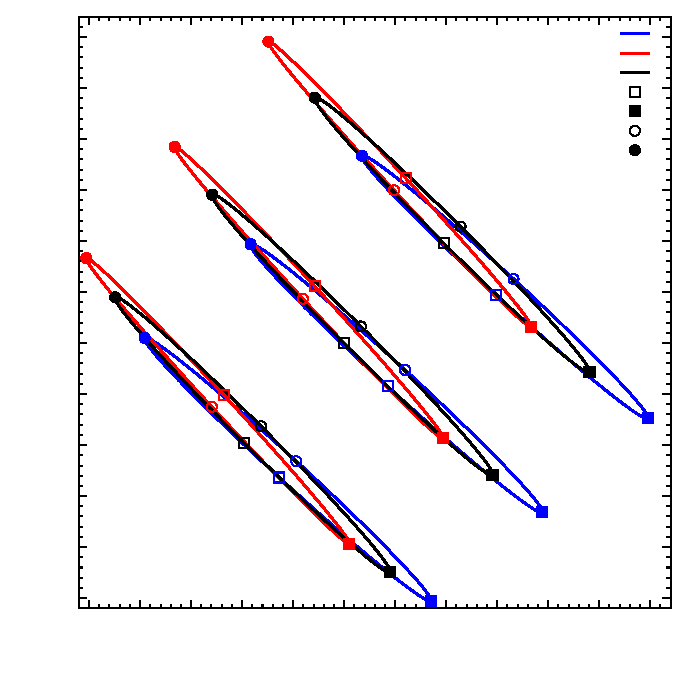
\includegraphics{pics/base_ball}}%
    \gplfronttext
  \end{picture}%
\endgroup
}
	\hfill
	\raisebox{2em}{\resizebox{0.50\linewidth}{!}{% GNUPLOT: LaTeX picture with Postscript
\begingroup
  \makeatletter
  \providecommand\color[2][]{%
    \GenericError{(gnuplot) \space\space\space\@spaces}{%
      Package color not loaded in conjunction with
      terminal option `colourtext'%
    }{See the gnuplot documentation for explanation.%
    }{Either use 'blacktext' in gnuplot or load the package
      color.sty in LaTeX.}%
    \renewcommand\color[2][]{}%
  }%
  \providecommand\includegraphics[2][]{%
    \GenericError{(gnuplot) \space\space\space\@spaces}{%
      Package graphicx or graphics not loaded%
    }{See the gnuplot documentation for explanation.%
    }{The gnuplot epslatex terminal needs graphicx.sty or graphics.sty.}%
    \renewcommand\includegraphics[2][]{}%
  }%
  \providecommand\rotatebox[2]{#2}%
  \@ifundefined{ifGPcolor}{%
    \newif\ifGPcolor
    \GPcolortrue
  }{}%
  \@ifundefined{ifGPblacktext}{%
    \newif\ifGPblacktext
    \GPblacktexttrue
  }{}%
  % define a \g@addto@macro without @ in the name:
  \let\gplgaddtomacro\g@addto@macro
  % define empty templates for all commands taking text:
  \gdef\gplbacktext{}%
  \gdef\gplfronttext{}%
  \makeatother
  \ifGPblacktext
    % no textcolor at all
    \def\colorrgb#1{}%
    \def\colorgray#1{}%
  \else
    % gray or color?
    \ifGPcolor
      \def\colorrgb#1{\color[rgb]{#1}}%
      \def\colorgray#1{\color[gray]{#1}}%
      \expandafter\def\csname LTw\endcsname{\color{white}}%
      \expandafter\def\csname LTb\endcsname{\color{black}}%
      \expandafter\def\csname LTa\endcsname{\color{black}}%
      \expandafter\def\csname LT0\endcsname{\color[rgb]{1,0,0}}%
      \expandafter\def\csname LT1\endcsname{\color[rgb]{0,1,0}}%
      \expandafter\def\csname LT2\endcsname{\color[rgb]{0,0,1}}%
      \expandafter\def\csname LT3\endcsname{\color[rgb]{1,0,1}}%
      \expandafter\def\csname LT4\endcsname{\color[rgb]{0,1,1}}%
      \expandafter\def\csname LT5\endcsname{\color[rgb]{1,1,0}}%
      \expandafter\def\csname LT6\endcsname{\color[rgb]{0,0,0}}%
      \expandafter\def\csname LT7\endcsname{\color[rgb]{1,0.3,0}}%
      \expandafter\def\csname LT8\endcsname{\color[rgb]{0.5,0.5,0.5}}%
    \else
      % gray
      \def\colorrgb#1{\color{black}}%
      \def\colorgray#1{\color[gray]{#1}}%
      \expandafter\def\csname LTw\endcsname{\color{white}}%
      \expandafter\def\csname LTb\endcsname{\color{black}}%
      \expandafter\def\csname LTa\endcsname{\color{black}}%
      \expandafter\def\csname LT0\endcsname{\color{black}}%
      \expandafter\def\csname LT1\endcsname{\color{black}}%
      \expandafter\def\csname LT2\endcsname{\color{black}}%
      \expandafter\def\csname LT3\endcsname{\color{black}}%
      \expandafter\def\csname LT4\endcsname{\color{black}}%
      \expandafter\def\csname LT5\endcsname{\color{black}}%
      \expandafter\def\csname LT6\endcsname{\color{black}}%
      \expandafter\def\csname LT7\endcsname{\color{black}}%
      \expandafter\def\csname LT8\endcsname{\color{black}}%
    \fi
  \fi
    \setlength{\unitlength}{0.0500bp}%
    \ifx\gptboxheight\undefined%
      \newlength{\gptboxheight}%
      \newlength{\gptboxwidth}%
      \newsavebox{\gptboxtext}%
    \fi%
    \setlength{\fboxrule}{0.5pt}%
    \setlength{\fboxsep}{1pt}%
\begin{picture}(7200.00,5040.00)%
    \gplgaddtomacro\gplbacktext{%
      \csname LTb\endcsname%%
      \put(645,595){\makebox(0,0)[r]{\strut{}-50}}%
      \csname LTb\endcsname%%
      \put(645,1021){\makebox(0,0)[r]{\strut{}-40}}%
      \csname LTb\endcsname%%
      \put(645,1447){\makebox(0,0)[r]{\strut{}-30}}%
      \csname LTb\endcsname%%
      \put(645,1872){\makebox(0,0)[r]{\strut{}-20}}%
      \csname LTb\endcsname%%
      \put(645,2298){\makebox(0,0)[r]{\strut{}-10}}%
      \csname LTb\endcsname%%
      \put(645,2724){\makebox(0,0)[r]{\strut{}0}}%
      \csname LTb\endcsname%%
      \put(645,3150){\makebox(0,0)[r]{\strut{}10}}%
      \csname LTb\endcsname%%
      \put(645,3576){\makebox(0,0)[r]{\strut{}20}}%
      \csname LTb\endcsname%%
      \put(645,4001){\makebox(0,0)[r]{\strut{}30}}%
      \csname LTb\endcsname%%
      \put(645,4427){\makebox(0,0)[r]{\strut{}40}}%
      \csname LTb\endcsname%%
      \put(645,4853){\makebox(0,0)[r]{\strut{}50}}%
      \csname LTb\endcsname%%
      \put(747,409){\makebox(0,0){\strut{}-1.00$\pi$}}%
      \csname LTb\endcsname%%
      \put(1515,409){\makebox(0,0){\strut{}-0.75$\pi$}}%
      \csname LTb\endcsname%%
      \put(2284,409){\makebox(0,0){\strut{}-0.50$\pi$}}%
      \csname LTb\endcsname%%
      \put(3052,409){\makebox(0,0){\strut{}-0.25$\pi$}}%
      \csname LTb\endcsname%%
      \put(3820,409){\makebox(0,0){\strut{}0.00$\pi$}}%
      \csname LTb\endcsname%%
      \put(4588,409){\makebox(0,0){\strut{}0.25$\pi$}}%
      \csname LTb\endcsname%%
      \put(5357,409){\makebox(0,0){\strut{}0.50$\pi$}}%
      \csname LTb\endcsname%%
      \put(6125,409){\makebox(0,0){\strut{}0.75$\pi$}}%
      \csname LTb\endcsname%%
      \put(6893,409){\makebox(0,0){\strut{}1.00$\pi$}}%
    }%
    \gplgaddtomacro\gplfronttext{%
      \csname LTb\endcsname%%
      \put(153,2724){\rotatebox{-270}{\makebox(0,0){\strut{}Normalised asymmetry $\mathcal{A}$ (\%)}}}%
      \csname LTb\endcsname%%
      \put(3820,130){\makebox(0,0){\strut{}$\delta_\text{CP}$}}%
      \csname LTb\endcsname%%
      \put(6309,4686){\makebox(0,0)[r]{\strut{}Normal hierarchy}}%
      \csname LTb\endcsname%%
      \put(6309,4500){\makebox(0,0)[r]{\strut{}Inverted hierarchy}}%
      \csname LTb\endcsname%%
      \put(6309,4314){\makebox(0,0)[r]{\strut{}Vacuum}}%
    }%
    \gplbacktext
    \put(0,0){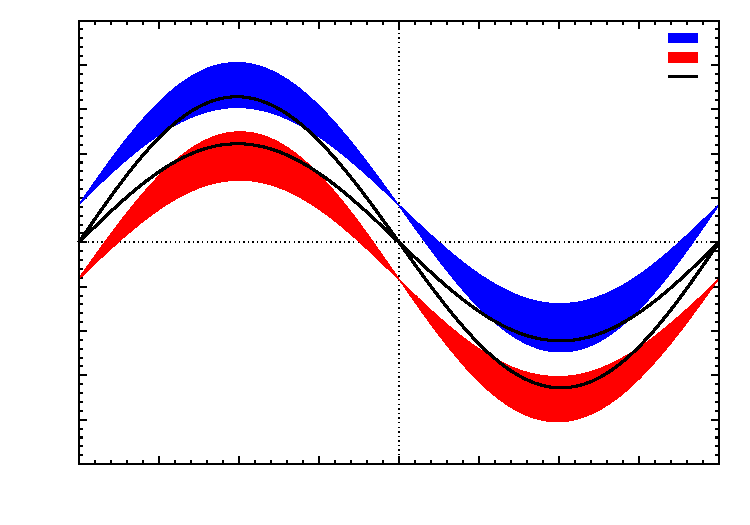
\includegraphics{pics/norm_asymm}}%
    \gplfronttext
  \end{picture}%
\endgroup
}}
	\caption{Effect of $\delta_\text{CP}$ on the oscillation probability.
		The oscillation probabilities for neutrinos and antineutrinos are plotted %
		against each other (left), while the CP phase is varied between $-\pi$ and $\pi$.
		The effect of $\sin^2\theta_{23}$ is also emphasised.
		The mass hierarchy has a non-negligible behaviour only if matter oscillation is %
		considered.
		The normalised asymmetry from Eq.~\ref{eq:asymmetry} is shown on the right.}
	\label{fig:baseball}
\end{figure}

Given the parametrisation in Eq.~\ref{eq:pmns}, %
this asymmetry is not measurable if the phase is trivial, \ie~$\delta_\text{CP} = 0$~or~$\pm \pi$, %
or if $\theta_{13}$ is vanishing.
From a model building point of view, however, a successful leptogenesis requires the parameters to satisfy %
$\qty|\sin\theta_{13} \sin\delta_\text{CP}| \gtrsim 0.09$
%\begin{equation}
%	\label{eq:leptogenesis}
%	\qty|\sin\theta_{13} \sin\delta_\text{CP}| \gtrsim 0.09\ ,
%\end{equation}
when the Majorana phases are vanishing~\cite{Pascoli:2006ci}.
The value of $\theta_{13}$ has been measured to be non-zero~\cite{Abe:2011sj,Abe:2011fz,An:2012eh,Ahn:2012nd} %
and for this reason it is expected that on-going and future generation neutrino experiments %
will also constrain the value of $\delta_\text{CP}$.


\section{Hyper-Kamiokande experiment}

\begin{figure}
	\centering
	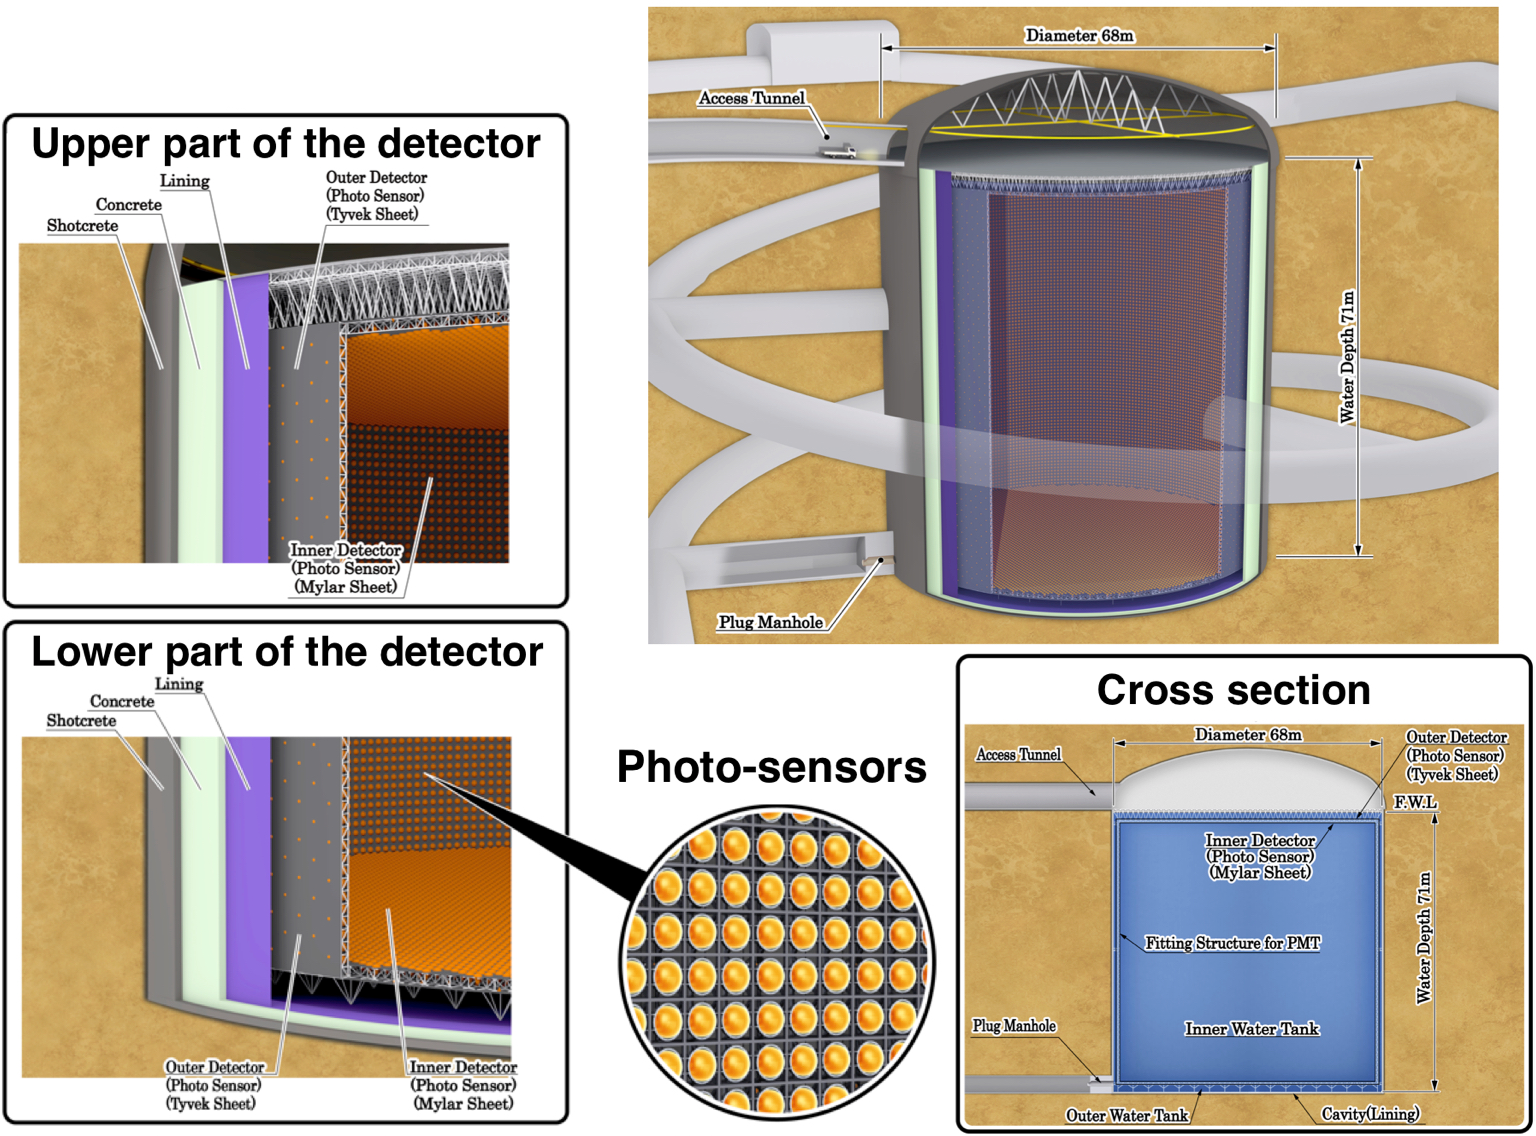
\includegraphics[width=0.8\linewidth]{pics/hkonlytank.png}
	\caption{Cut-view of the Hyper-Kamiokande experiment.}
	\label{fig:hkdr}
\end{figure}

Hyper-Kamiokande (HK)~\cite{Abe:2018uyc} will be the next-generation water Cherenkov detector, %
superseding its predecessor, Super-Kamiokande (SK).
Employing ring-imaging technique, the rare interactions of neutrinos can be detected, %
as well as the possible spontaneous decay of nucleons.
The design of HK does not deviate much from SK and Kamiokande.
The cylindrical tank of HK will be 72\,m high and 68\,m in diameter, with a fiducial volume of 188.4\,kton (total volume 257.8\,kton), %
around 8.4 times the fiducial volume of SK.
The photo-coverage of the inner detector region will be 40\,\%, the same of SK, %
but it translates to roughly forty thousands photomultipliers (PMTs).
New 20''box and line PMTs will be employed, with improved charge and riming resolution, thanks to the increased quantum efficiency %
which is almost twice the QE of previous PMT generation.
It also has the high pressure tolerance for the usage below 60 m depth of water.
A study for implementing multi PMT modules, containing each 23 3'' PMT, is being carried out
The detector will be located underground at Kamioka mine in Gifu Prefecture, %
with an overburden of approximately 650 meters or more of rock, which is equivalent to \np{1750} meters or more of water.

Thanks to incredible statistics and cutting edge resolutions, HK will be capable of a vast variety of physics studies, %
from accelerator and atmospheric neutrinos to solar and supernova neutrinos.
Besides detecting proton decay, the main goal of HK is to measure~$\delta_\text{CP}$ and constrain the other oscillation parameters %
with high precision.
This is achievable by studying accelerator neutrinos, and to this end the possibility of installing a second detector in Korea, %
at the secondary oscillation peak, is being investigated.

HK will be located 295\,km away from the target and $2.5^\circ$ off-axis with respect to the beamline.
The detector cavity is planed to be excavated in Mt. Nijugo-yama in the Tochibora-mine in Gifu Prefecture, %
which is approximately 8\,km south from SK.
The neutrino beam is generated by a 30\,GeV proton beam colliding on a fixed graphite target; %
a`focusing horn selects positively charged ($\nu$ mode) or negatively charged ($\cj{\nu}$ mode) pions, %
which decay leptonically, to obtain an almost pure muon neutrino or antineutrino beam, peaking at 600\,MeV.
The accelerator facility at J-PARC will undergo a planned upgrade to increase the beam power up to 1.3\,MW, %
before HK starts operation.
The T2K near detector system, comprised of the two modules ND280 and INGRID, will be refurbished %
and the new Intermediate Water Cherenkov Detector, possibly gadolinium-loaded, will be located %
around 1\,km from the target.

HK will take data for ten years, collecting a total of \np{2.7e22} Protons On Target, %
divided between $\nu$ and $\cj{\nu}$ beam modes.
Studies have shown that CP violation discovery is not very sensitive to the time ratio between the two modes (ref?).
Assuming $\nu:\cj{\nu} = 1:3$ and $\delta_\text{CP} = 0$, %
the expected number of fully-contained events in the fiducial volume for the channels %
$\nu_\mu \to \nu_e$ and $\cj{\nu}_\mu \to \cj{\nu}_e$ %
are respectively \np{1643} and \np{15} in $\nu$ mode and \np{206} and \np{1183} in $\cj{\nu}$ mode, %
assuming CP conservation.
Deviations from these expected numbers could be indication of CP violation.
%A preliminary study for the HK design report~\cite{Abe:2018uyc}, using a different analysis, %
%estimated a significance well-above $5\,\sigma$ after ten years of data taking, as can be seen in Fig.~\ref{fig:hkdr}.
The project has been recentely approved by japanese goverment and data taking is expected commencing by 2027.

The uncertainty of the Earth’s density between Tokai and Kamioka is estimated to be at most 6\% [181].
Because the matter effect contribution to the total $\nu_\mu \to \nu_e$ appearance probability is %
less than 10\% for 295km baseline, the uncertainty from the matter density is estimated to be less
than 0.6\% and neglected in the following analysis.


\section{Sensitivity studies}

At any stage of the experiment it is important to asses the impact of systematic errors on the total sensitivity of HK.
One of the main goal is to constrain with high precision oscillation parameters, especially $\delta_\text{CP}$ and %
and the octant determination.
Even if real data is not available, it is possible to understand whether the statistics collected have %
enough constraining power to achieve the target precision.
The oscillation parameters and systematic uncertainties are input to a Monte Carlo simulation %
to build expected distribution of events.
This expected data is then compared to simulated \emph{observed data}, which is created by selecting %
a combination of oscillation parameters in order to mimic the real distributions of event that will be collected eventually.
Scanning over the oscillation parameters, the resolution of HK to oscillation parameters and, more importantly, %
the influence of the systematic uncertainties can be studied.
%To this end, a fitting framework is employed, capable of performing to study Monte Carlo simulation of beam and atmospheric samples. 

\subsection{Event samples}

\begin{table}
	\centering
	\caption{Samples event for atmospheric data. They are categorised as fully-contained sub-GeV (FC sub-GeV), %
		fully-contained multi-GeV (FC multi-GeV), partially-contained (PC) and upward-going muons (UP-$\mu$).}
	\label{tab:atmo_samples}
	\begin{tabular}{llcc}
		\toprule
		Event type	&	Sample	&	Bins $\log p$	& Bins $\cos\theta$  \\
		\midrule
		\multirow{7}{*}{\bf FC sub-GeV}	& one ring $e$-like and 0 decay-$e$	& 13 & 20 \\
						& one ring $e$-like and 1 decay-$e$	& 13 & 2 \\
						& one ring $\mu$-like and 0 decay-$e$	& 13 & 20 \\
						& one ring $\mu$-like and 1 decay-$e$	& 13 & 20\\
						& one ring $\mu$-like and 2 decay-$e$	& 13 & 2 \\
						& one ring $\pi^0$			& 13 & 2 \\
						& two rings $\pi^0$			& 5 & 2 \\
		\midrule
		\multirow{7}{*}{\bf FC multi-GeV}& one ring $\nu_e$-like     	& 10 & 20 \\
						& one ring $\cj{\nu}_e$-like    & 10 & 20 \\
						& one ring $\nu_\mu$-like       & 5 & 20 \\
						& multi ring $\nu_e$-like       & 8 & 20 \\
						& multi ring $\cj{\nu}_e$-like  & 8 & 20 \\
						& multi ring $\nu_\mu$-like     & 4 & 20 \\
						& multi ring other		& 10 & 20 \\
		\midrule
		\multirow{2}{*}{\bf PC}		& stopping 			& 4 & 20 \\
						& through-going 		& 5 & 20 \\
		\midrule
		\multirow{3}{*}{\bf UP-$\mu$}	& stopping 			& 4 & 20 \\
						& through-going, not showering 	& 1 & 20 \\
						& through-going, showering 	& 1 & 20 \\
		\bottomrule
	\end{tabular}
\end{table}

For the study, SK atmospheric Monte Carlo (MC) is adapted and scaled to HK statistics to compose the atmospheric sample.
A total of \np{2224} bins are used, divided in several two-dimensional histograms of $\log p$ and $\cos\vartheta$, %
where $\vartheta$ is the azimuthal angle.
These are divided in the usual categories of fully-contained, partially-contained, and upward-going muons, %
and are summarised in~\reftab{tab:atmo_samples}~\cite{Jiang:2019xwn}.
The beam sample, instead, is created using the far detector flux predicted with NEUT.
From the flux prediction, fully-contained candidate events in the fiducial volume are grouped %
as appeareance signal, i.e.\ $\nu_\mu\to\nu_e$ and $\cj{\nu}_\mu\to\cj{\nu}_e$, %
and background, i.e.\ unoscillated neutrinos.
Signal and background distributions in true energy (98 bins) undergo event selection criteria %
to obtain the distributions in reconstructed energy (87 bins) for the four event samples:
\begin{multicols}{2}
	\begin{itemize}
		\item one ring $e$-like in $\nu$-mode,
		\item one ring $\mu$-like in $\nu$-mode,
		\item one ring $e$-like in $\cj{\nu}$-mode,
		\item one ring $\mu$-like in $\cj{\nu}$-mode.
	\end{itemize}
\end{multicols}
We do not consider the one $e$-like + one electron decay sample in this study.
A set of 2D smearing matrices, produced by the T2K fitting framework VALOR, %
simulates and replaces the correct event selection process, including tuning of the flux with near detector constraints.
These smearing matrices are provided for all samples, acting on signal (CCQE and CCnQE) %
and background (CCQE, CCnQE, and NC) distributions.


\subsection{Systematic model}

There are 67 systematics for the atmospheric sample, adopted from SK atmospheric studies~\cite{Abe:2017aap}.
List systematics in appendix.
A more accurate systematic study for the atmospheric analysis of HK is expected in the future.
The atmospheric systematics are initally uncorrelated with the beam systematics.
The focus of this work is the beam sample.

\begin{figure}
	\centering
	\resizebox{0.9\linewidth}{!}{% GNUPLOT: LaTeX picture with Postscript
\begingroup
  \makeatletter
  \providecommand\color[2][]{%
    \GenericError{(gnuplot) \space\space\space\@spaces}{%
      Package color not loaded in conjunction with
      terminal option `colourtext'%
    }{See the gnuplot documentation for explanation.%
    }{Either use 'blacktext' in gnuplot or load the package
      color.sty in LaTeX.}%
    \renewcommand\color[2][]{}%
  }%
  \providecommand\includegraphics[2][]{%
    \GenericError{(gnuplot) \space\space\space\@spaces}{%
      Package graphicx or graphics not loaded%
    }{See the gnuplot documentation for explanation.%
    }{The gnuplot epslatex terminal needs graphicx.sty or graphics.sty.}%
    \renewcommand\includegraphics[2][]{}%
  }%
  \providecommand\rotatebox[2]{#2}%
  \@ifundefined{ifGPcolor}{%
    \newif\ifGPcolor
    \GPcolortrue
  }{}%
  \@ifundefined{ifGPblacktext}{%
    \newif\ifGPblacktext
    \GPblacktexttrue
  }{}%
  % define a \g@addto@macro without @ in the name:
  \let\gplgaddtomacro\g@addto@macro
  % define empty templates for all commands taking text:
  \gdef\gplbacktext{}%
  \gdef\gplfronttext{}%
  \makeatother
  \ifGPblacktext
    % no textcolor at all
    \def\colorrgb#1{}%
    \def\colorgray#1{}%
  \else
    % gray or color?
    \ifGPcolor
      \def\colorrgb#1{\color[rgb]{#1}}%
      \def\colorgray#1{\color[gray]{#1}}%
      \expandafter\def\csname LTw\endcsname{\color{white}}%
      \expandafter\def\csname LTb\endcsname{\color{black}}%
      \expandafter\def\csname LTa\endcsname{\color{black}}%
      \expandafter\def\csname LT0\endcsname{\color[rgb]{1,0,0}}%
      \expandafter\def\csname LT1\endcsname{\color[rgb]{0,1,0}}%
      \expandafter\def\csname LT2\endcsname{\color[rgb]{0,0,1}}%
      \expandafter\def\csname LT3\endcsname{\color[rgb]{1,0,1}}%
      \expandafter\def\csname LT4\endcsname{\color[rgb]{0,1,1}}%
      \expandafter\def\csname LT5\endcsname{\color[rgb]{1,1,0}}%
      \expandafter\def\csname LT6\endcsname{\color[rgb]{0,0,0}}%
      \expandafter\def\csname LT7\endcsname{\color[rgb]{1,0.3,0}}%
      \expandafter\def\csname LT8\endcsname{\color[rgb]{0.5,0.5,0.5}}%
    \else
      % gray
      \def\colorrgb#1{\color{black}}%
      \def\colorgray#1{\color[gray]{#1}}%
      \expandafter\def\csname LTw\endcsname{\color{white}}%
      \expandafter\def\csname LTb\endcsname{\color{black}}%
      \expandafter\def\csname LTa\endcsname{\color{black}}%
      \expandafter\def\csname LT0\endcsname{\color{black}}%
      \expandafter\def\csname LT1\endcsname{\color{black}}%
      \expandafter\def\csname LT2\endcsname{\color{black}}%
      \expandafter\def\csname LT3\endcsname{\color{black}}%
      \expandafter\def\csname LT4\endcsname{\color{black}}%
      \expandafter\def\csname LT5\endcsname{\color{black}}%
      \expandafter\def\csname LT6\endcsname{\color{black}}%
      \expandafter\def\csname LT7\endcsname{\color{black}}%
      \expandafter\def\csname LT8\endcsname{\color{black}}%
    \fi
  \fi
    \setlength{\unitlength}{0.0500bp}%
    \ifx\gptboxheight\undefined%
      \newlength{\gptboxheight}%
      \newlength{\gptboxwidth}%
      \newsavebox{\gptboxtext}%
    \fi%
    \setlength{\fboxrule}{0.5pt}%
    \setlength{\fboxsep}{1pt}%
\begin{picture}(10800.00,9360.00)%
    \gplgaddtomacro\gplbacktext{%
    }%
    \gplgaddtomacro\gplfronttext{%
      \csname LTb\endcsname%%
      \put(10087,93){\makebox(0,0)[l]{\strut{}$-1$}}%
      \csname LTb\endcsname%%
      \put(10087,1010){\makebox(0,0)[l]{\strut{}$-0.8$}}%
      \csname LTb\endcsname%%
      \put(10087,1927){\makebox(0,0)[l]{\strut{}$-0.6$}}%
      \csname LTb\endcsname%%
      \put(10087,2844){\makebox(0,0)[l]{\strut{}$-0.4$}}%
      \csname LTb\endcsname%%
      \put(10087,3762){\makebox(0,0)[l]{\strut{}$-0.2$}}%
      \csname LTb\endcsname%%
      \put(10087,4679){\makebox(0,0)[l]{\strut{}$0$}}%
      \csname LTb\endcsname%%
      \put(10087,5596){\makebox(0,0)[l]{\strut{}$0.2$}}%
      \csname LTb\endcsname%%
      \put(10087,6514){\makebox(0,0)[l]{\strut{}$0.4$}}%
      \csname LTb\endcsname%%
      \put(10087,7431){\makebox(0,0)[l]{\strut{}$0.6$}}%
      \csname LTb\endcsname%%
      \put(10087,8348){\makebox(0,0)[l]{\strut{}$0.8$}}%
      \csname LTb\endcsname%%
      \put(10087,9266){\makebox(0,0)[l]{\strut{}$1$}}%
    }%
    \gplbacktext
    \put(0,0){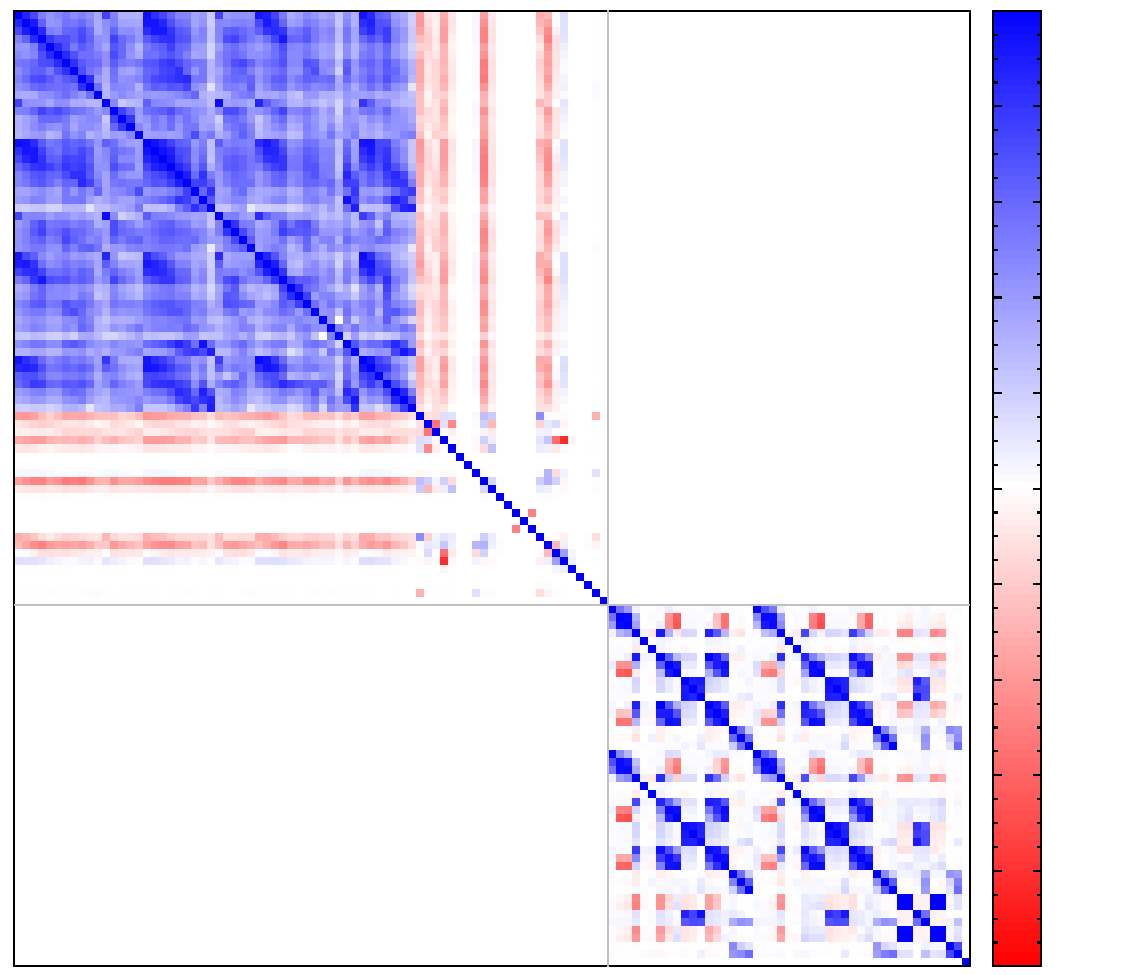
\includegraphics{pics/matrixplot}}%
    \gplfronttext
  \end{picture}%
\endgroup
}
	\caption{Correlation matrix of the beam systematic model.
		The two main blocks correspond to respectively the BANFF errors and the far detector %
		Final State interaction errors.}
	\label{fig:correlation}
\end{figure}

For the beam part, the T2K 2018 error model is employed~\cite{Abe:2018wpn}.
There are 74 uncertainties for flux and cross-section parameters, from near detector constraints, %
known as the BANFF fit. %
divided in $25\times 2$ systematics, for each beam mode, for the four main flux components, %
They are grouped in 50 systematics---25 for the $\nu$ mode and 25 for the $\cj{\nu}$~mode---%
for the main flux components ($\nu_e$, $\nu_\mu$, $\cj{\nu}_e$, and $\cj{\nu}_\mu$), % 
and 24 systematics for cross-section parameters.
There are also 45 uncertainties for SK detector efficiencies and Final State Interactions,
which parameterise the uncertainties on the four final state event selections at the far detector: %
1 ring $e$-like and 1 ring $\mu$-like in both $\nu$ and $\cj{\nu}$ modes.
The 1 ring $e$-like + 1 electron decay sample is not treated in this study.
Among these, one systematic describes the energy scale uncertainty.
It consists of 25 systematic uncertainities, constrained by near detector fits, for each beam mode---neutrino or antineutrino---describing %
are described by 25 systematics for each beam mode---neutrino or antineutrino.
There are 24 errors that describe cross-section parameters, also constrained by near detector data.
from flux and cross-section parameters constrained by near detector fits.
Among the flux and cross-section parameters, These For the four main flux components 
25 uncertainties for the beam in neutrino mode and 25 for the antineutrino mode.
($2p2h$ normalisation and shape for \tapi{16}O, CCQE axial-mass scaling factor, CC and NC interaction normalisations, %
RPA coefficients, binding energy on oxygen).
In addition, there are 45 systematics from SK detector efficiencies and Final State Interactions, %
which parameterise the uncertainties on the four final state interaction types %
at the far detector: %
1 ring $e$-like and 1 ring $\mu$-like in both $\nu$ and $\cj{\nu}$ modes.

One systematic is adopted to describe the energy scale uncertainty at the far detector.
The reconstruction of the momenta in a neutrino event is mainly based on the charge collected by the PMTs, %
and therefore the resolution is limited by water quality and PMT gain.
A precise momentum determination of the incoming neutrino is a necessary requirement for oscillation analysis.
The calibration of the energy scale of SK is performed using four well-known independent control samples~\cite{Abe:2017aap}.
%from 1\,GeV to 10\,GeV by high energy stopping muons; from 200\,MeV to 500\,MeV by low energy stopping muons;
%around 130\,MeV by neutral pions from neutrino interactions; %
%around 40\,MeV from decay electrons.
Since the energy loss $\dv*{E}{x}$ is approximately constant, %
the ratio between reconstructed momentum and track length of high energy stopping muon  %
is used to regulate the energy scale for energes in the range 1--10\,GeV.
The track is estimated from the entering position of the muon and the vertex of the detected Michel electron, %
both of which are assumed to be independent on the reconstruction mehtod.
The momentum of low-energy stopping muons with energies from 200\,MeV to 500\,MeV are estimated by determining the %
Cherenkov angle using \refeqs{eq:cherenkov_threshold}{eq:cherenkov_angle}; %
only events with a clear Cherenkov ring and optimal reconstruction are selected, %
and the purity of the sample is improved by requiring the detection of the decay electron in the fiducial volume.
The single neutral pions produced in NC interactions of atmospheric neutrinos are reconstructed %
by looking at the invariant mass of the final state photons
\begin{equation}
	m_{\pi^0}^2 = 2\,p_{\gamma_1}\,p_{\gamma_2} (1-\cos\theta)\ ,
\end{equation}
with $\theta$ the opening angle between $\gamma_1$ and $\gamma_2$.
The error of the energy scale at around 130\,MeV comes from comparing the peak positions of $m_{\pi^0}$ %
between data and simulation.
Finally, the distribution of decay electron events from stopping cosmic muons is used at energies around 40\,MeV.
This sample is used to test whether the detector response is uniform, since %
verteces and the direction of the electrons distribute homogenously and isotropically in the fiducial volume.
The stability in time of the energy scale is instead validated by the high energy stopping muons.


\subsection{Oscillation space}

\begin{table}
	\small
	\centering
	\caption{Oscillation space.}
	\label{tab:osc_space}
	\begin{tabular}{cccc}
		\toprule
		Parameter				& Nominal	& Range	& Points \\
		\midrule
		$\Delta m_{12}^2/\np{e-5}\,\text{eV}^2$	& 7.53		& --			& fixed	\\
		$\sin^2 2\theta_{12}$			& 0.8463	& --			& fixed	\\
		\midrule
		$\Delta m_{23}^2/\np{e-3}\,\text{eV}^2$	& 2.509		& [2.464:2.554]		& 13	\\
		$\sin^2 2\theta_{13}$			& 0.085		& [0.070:0.100]		& 13	\\
		$\sin^2 \theta_{23}$			& 0.528		& [0.426:0.579]		& 19	\\
		$\delta_\text{CP}$			& $-\pi/2$	& [$-\pi$:$\pi$]	& 61	\\
		\bottomrule
	\end{tabular}
\end{table}


Both the atmospheric and beam distributions are weighted by the corresponding oscillation probabilities.
For the study of this thesis, the oscillation parameters are scanned over the space
The oscillation space spans four variables, $\Delta m^2_{32}$, $\sin^2 2\theta_{13}$, $\sin^2 \theta_{23}$, and %
$\delta_\text{CP}$, on a grid of respectively $13\,\times\,13\,\times\,19\,\times\,61$ points.
The solar squared mass difference and the solar angle are fixed.
Apart from $\delta_\text{CP}$ which is scanned over all possible values, %
the intervals for the other parameters are built around ``Asimov A'', the nominal T2K best fit point~\cite{Abe:2017vif} .
The oscillation space is listed in \reftab{tab:osc_space}.
For the atmospheric squared mass difference and the reactor angle, the range is chosen such that it covers %
a $[-3\sigma, +3\sigma]$ interval, where $\sigma$ is the error from the Asimov A set; %
the range for $\sin^2\theta_{23}$ spans over $[-6\sigma, +3\sigma]$ so that both octants are covered.
Reactor experiments~\cite{Bak:2018ydk, Adey:2018zwh}.
At each point of this space, the event distributions are weighted with the correct oscillation probability %
for appearance or disappearance channels.
A special point of the parameter space is chosen as a \emph{true} combination of oscillation parameters %
to perform sensitivity studies using a $\chi^2$-test statistics.
By changing the \emph{true} point, it is possible to define the exclusion regions for CP violation, %
by comparing the $\chi^2$ at any value of $\delta_\text{CP}$ with the $\chi^2$ computed at %
the null hypothesis, i.e.\ CP conservation.
The sensitivity to exclude the $\sin \delta_\text{CP} = 0$ as a function of \emph{true} $\delta_\text{CP}$ %
is quantified by %
\begin{equation}
	\sigma = \sqrt{\min_{\delta_\text{CP} = 0,\pm\pi}\! \chi^2\  -\,\chi^2_\text{\emph{true}}}\ ,
\end{equation}
where $\chi^2_\text{\emph{true}}$ is evaluated at the \emph{true} point.

\subsection{Test statistic}

We define the likelihood
\begin{equation}
	\mathfrak{L}(E_n, O_n) = \prod_n \frac{e^{-E_n} O_n^{E_n}}{O_n!}\ ,
\end{equation}
where $O_n$ and $E_n$ are respectively the number of observed and expected events in the $n$-th bin, %
which are built using oscillation parameters $\vartheta$.
The expected events are defined by a prediction of events at the far detector weighted by the oscillation probabilities %
for parameters $\vartheta$, and, since there is no real data yet, the ``observed'' events are also given by %
a prediction at the \emph{true} oscillation point $\vartheta_\text{true}$.
%and the product runs over the total number of bins.
The $\chi^2$ is hence the following log-likelihood ratio
\begin{equation}
	\label{eq:log_ratio}
	\chi^2(\vartheta) = -2 \log \qty[\frac{\mathfrak{L}(E_n, O_n)}{\mathfrak{L}(O_n, O_n)}] =
		2 \sum_n \qty[E_n - O_n + O_n \log \qty(\frac{E_n}{O_n})]\ ,
\end{equation}
and it is modified according to the ``pull approach'' $\chi^2$~\cite{Fogli:2002pt}: %
the parameters $\uj{\varepsilon}$ are introduced to account for systematic uncertainties, by replacing
\begin{equation}
	\label{eq:pull}
	E_n\ \longrightarrow\ E_n\,\qty(1 + \textstyle\sum_j f_j^n \varepsilon_j)\ ,
\end{equation}
and a penalty term that includes variances and covariances of such parameters is added to the likelihood.
The $\chi^2$ becomes the following
%\begin{align}
%	\chi^2_\text{tot} &=\ \chi^2_\text{obs}\ +\ \chi^2_\text{syst} \notag\\
%	&= \overset{\text{obs}}{2 \sum_n \qty[E_n(1+{\textstyle\sum_j f_j^n \varepsilon_j}) - O_n + O_n \log \qty(\frac{E_n(1+\sum_j f_j^n \varepsilon_j)}{O_n})]} + %
%	\overset{\text{\shortstack{syst\\ \hphantom{.}}}}{\sum_{ij} \varepsilon_i\, \rho^{-1}_{ij}\, \varepsilon_j}\ ,
%\end{align}
\begin{equation}
	\label{eq:chi2}
	\chi^2(\vartheta;\uj{\epsilon})  = 2 \sum_n \qty[E_n(1+{\textstyle\sum_j f_j^n \varepsilon_j}) - O_n + %
		O_n \log \qty(\frac{E_n(1+\sum_j f_j^n \varepsilon_j)}{O_n})] + %
		\sum_{ij} \varepsilon_i\, \rho^{-1}_{ij}\, \varepsilon_j\ ,
\end{equation}
where $\rho^{-1}$ is the inverse of the correlation matrix of the systematic errors.
The effect of the systematic uncertainties on the event distributions are embedded in the $f_j^n$ parameters, %
defined as the fractional change induced on the $n$-th bin by a 1\,$\sigma$ variation of the $j$-th systematic.
The amount of change is therefore parametrised by $\varepsilon_j$ in units of the uncertainty $\sigma_j$.
However, being $\rho$ the correlation matrix, the $\varepsilon_j$ are promoted to embody the systematic uncertainties.
Once defined the observed sample, the oscillation parameters $\vartheta$ are scanned over the oscillation %
space defined in \reftab{tab:osc_space} and the $\chi^2$ is then profiled it with respect to the parameters $\uj{\varepsilon}$:
\begin{equation}
	\label{eq:chi2_min}
	\chi^2(\vartheta) = \min_{\uj{\varepsilon}}\, \qty\Big[\,\chi^2(\vartheta;\uj{\varepsilon})\,]\ ,
\end{equation}
The minimisation of the $\chi^2$ leads to a set of $j$ non-linear equations %,
which can be solved iteratively if the condition $\sum_j f^n_j \varepsilon_j < 1$~holds.
\begin{equation}
	\pdv{\chi^2}{\varepsilon_j} (\vartheta;\uj{\varepsilon}) = 0\ .
\end{equation}
The system can be solved with the Newton's method by finding the Hessian of the $\chi^2$.
This gives a linear system, which can be iterated until sufficient precision is achieved
%The algorithm is stabilised by means of the Levenberg-Marquardt algorithm
\begin{equation}
	\pdv{\chi^2(\uj{\varepsilon}^{(n)})}{\varepsilon_k}{\varepsilon_j} %
	\cdot \qty(\varepsilon_j^{(n+1)} - \varepsilon_j^{(n)}) = %
	-\pdv{\chi^2(\uj{\varepsilon}^{(n)})}{\varepsilon_k}\ ,
\end{equation}
with $(n)$ the iteration index.
The Gauss-Newton's algorithm can sometimes be unstable, especially with a large number of parameters, %
due to its fast convergence.
The algorithm is typically improved by adopting the Lavenberg-Marquardt method~\cite{Levenberg_1944, Marquardt_1963} %
which modifies the Hessian in the following way
\begin{equation}
	\qty[\pdv{\chi^2(\uj{\varepsilon}^{(n)})}{\varepsilon_k}{\varepsilon_j} %
	+ \lambda \max \qty(\text{diag} \pdv{\chi^2(\uj{\varepsilon}^{(n)})}{\varepsilon_k}{\varepsilon_j}) \mathbb{1}]
	\cdot \qty(\varepsilon_j^{(n+1)} - \varepsilon_j^{(n)}) = %
	-\pdv{\chi^2(\uj{\varepsilon}^{(n)})}{\varepsilon_k}\ ,
\end{equation}
where $\lambda$ is a parameter chosen dynamically: if the cost function $\chi^2$ decreases %
after an iteratio nstep, then $\lambda$ is reduced; otherwise $\lambda$ is increased and the step re-computed.
In the limit $\lambda \to 0$, the algorithm approximates the Gauss-Newton's method and its fast convergence.
When $\lambda$ is large, the linear system resembles a gradient descent with small steps of the order of $\lambda^{-1}$, %
but a more stable convergence.
We adopt a ``delayed-gratification scheme'' for $\lambda$~\cite{Transtrum2012}, using an inital value of $\lambda^{(0)} = 1$ and finding %
an optimal increment and decrement of respectively $\lambda^{(n+1)} = 5\,\lambda^{(n)}$ and $\lambda^{(n+1)} = \lambda^{(n)} / 10$.

To account for future constraints from other experiments, a gaussian penalty terms is added %
to the minimised value of $\chi^2$ from \refeq{eq:chi2_min}
\begin{equation}
	\chi^2_\text{penalty} = \frac{(\vartheta - \hat{\vartheta})^2}{\sigma_\vartheta^2}\ .
\end{equation}
The current constraint applied comes from the measurement of $\theta_{13}$ by future reactor experiments, %
that are predicted to achieve $\sigma(\sin^2 2\theta_{13}) = 0.005$.

For most of the systematic parameters, a linear response is assumed in the~MC.
This means that varying of the $j$-th systematic by a known amount, $\beta_j \to \beta_j + \varepsilon_j\sigma_j$, %
the number of expected events changes:
\begin{align*}
	\beta_j\ \overset{\scriptstyle \text{MC}}{\longmapsto}\ E_n %
	%\qquad \overset{\varepsilon_j \sigma_j}{\Longrightarrow} \qquad %
	\qquad \Longrightarrow \qquad %
	\beta_j + \varepsilon_j\sigma_j\ \overset{\text{MC}}{\longmapsto}\ E_n ( 1 + \varepsilon_j f_n ^j )\ .
	%&\hspace{0.4em}\text{\scriptsize MC} \\
	%\text{\scriptsize MC\ :} \hspace{1em} \Downarrow & \hspace{3.5em} \Downarrow	\\	
\end{align*}
Certain systematic uncertainties, such as the CCQE axial-mass scaling factor, the Fermi momentum for \tapi{16}O, %
or some of the RPA coefficients\footnote{The Random Phase Approximation (RPA) method is applied to calculate the total cross-sections %
	of electron neutrinos on nuclei.}, 
do not present a linear behaviour for small values of $\varepsilon$ %
and they are better described by a four-point linear interpolation of different~$f_j^n$ histograms, %
computed at~$\pm1\,\sigma$ and~$\pm3\,\sigma$ variations of the systematic parameter.

\section{Systematic studies}

It is expected that larger systematic errors will result in a worse sensitivity,
but certain uncertainties affect the measurement of the oscillation parameters more than others.
For example, these can be the uncertainties on $\nu_e$ and $\cj{\nu}_e$ charged-current cross-sections, %
the transverse flux model, the pion absorption probability, the total energy scale in SK, or the flux alignment.
We study the impact of some selected systematics by modifying the nominal systematic model %
and analysing the overall predicted sensitivity of the experiment in these different scenarios.
Doing so, it is possible to determine which systematics have the most important repercussion on the sensitivity,
since it is fundamental to understand their effect at all phases of the experiment.

\subsection{Validation of the fitter}

To validate the fitting framework a special systematic set for the beam sample is used.
It is composed of just two systematics: the $\nu_e$ and the $\cj{\nu_e}$ CC cross-section uncertainties.
These two errors are either correlated or anti-correlated %
and they are tested at different value (1\%, 2\%, 3\%, 4\%, and 5\%) for a total of ten fits.
Given the definition of $\chi^2$ in \refeq{eq:chi2}, %
the difference in the fits is just the correlation matrix at a given relative error, %
whereas the difference is provided by the $1\sigma$ histograms at fixed correlation.
The correlation matrices used are simply
\begin{equation}
	\rho = \mqty(1 & 1 \\ 1 & 1) \quad\text{and}\quad
	\rho = \mqty(1 & -1 \\ -1 & 1) \ ,
\end{equation}
but they are both singular and not invertible.
A small offset of \np{e-5} is added to off-diagonal terms to allow the calculation of the $\chi^2$.

The prediction of the one ring $e$-like samples in $\nu$-mode and $\cj{\nu}$-mode are shown in \reffig{fig:nuenorm_prediction} %
for respectively the $\nu_e$ and the $\cj{\nu_e}$ CC cross-section uncertainties applied individually.
The effect of the systematic error at different magnitudes of the relative error scales linearly.

The importance of this systematic set can be appreciated in \reffig{fig:nuenorm_sensitivity}.
When the two CC cross-sections are anti-correlated, the increment of one error brings about the decrement of the other.
This results in an effective fluctuation of the number of events, exhibiting a CP violation--like phenomenon.
A large systematic uncertainty of such anti-correlated cross-section parameters can therefore only aggravate the %
overall sensitivity to $\delta_\text{CP}$.

\begin{figure}
	\centering
	\resizebox{0.475\linewidth}{!}{% GNUPLOT: LaTeX picture with Postscript
\begingroup
  \makeatletter
  \providecommand\color[2][]{%
    \GenericError{(gnuplot) \space\space\space\@spaces}{%
      Package color not loaded in conjunction with
      terminal option `colourtext'%
    }{See the gnuplot documentation for explanation.%
    }{Either use 'blacktext' in gnuplot or load the package
      color.sty in LaTeX.}%
    \renewcommand\color[2][]{}%
  }%
  \providecommand\includegraphics[2][]{%
    \GenericError{(gnuplot) \space\space\space\@spaces}{%
      Package graphicx or graphics not loaded%
    }{See the gnuplot documentation for explanation.%
    }{The gnuplot epslatex terminal needs graphicx.sty or graphics.sty.}%
    \renewcommand\includegraphics[2][]{}%
  }%
  \providecommand\rotatebox[2]{#2}%
  \@ifundefined{ifGPcolor}{%
    \newif\ifGPcolor
    \GPcolortrue
  }{}%
  \@ifundefined{ifGPblacktext}{%
    \newif\ifGPblacktext
    \GPblacktexttrue
  }{}%
  % define a \g@addto@macro without @ in the name:
  \let\gplgaddtomacro\g@addto@macro
  % define empty templates for all commands taking text:
  \gdef\gplbacktext{}%
  \gdef\gplfronttext{}%
  \makeatother
  \ifGPblacktext
    % no textcolor at all
    \def\colorrgb#1{}%
    \def\colorgray#1{}%
  \else
    % gray or color?
    \ifGPcolor
      \def\colorrgb#1{\color[rgb]{#1}}%
      \def\colorgray#1{\color[gray]{#1}}%
      \expandafter\def\csname LTw\endcsname{\color{white}}%
      \expandafter\def\csname LTb\endcsname{\color{black}}%
      \expandafter\def\csname LTa\endcsname{\color{black}}%
      \expandafter\def\csname LT0\endcsname{\color[rgb]{1,0,0}}%
      \expandafter\def\csname LT1\endcsname{\color[rgb]{0,1,0}}%
      \expandafter\def\csname LT2\endcsname{\color[rgb]{0,0,1}}%
      \expandafter\def\csname LT3\endcsname{\color[rgb]{1,0,1}}%
      \expandafter\def\csname LT4\endcsname{\color[rgb]{0,1,1}}%
      \expandafter\def\csname LT5\endcsname{\color[rgb]{1,1,0}}%
      \expandafter\def\csname LT6\endcsname{\color[rgb]{0,0,0}}%
      \expandafter\def\csname LT7\endcsname{\color[rgb]{1,0.3,0}}%
      \expandafter\def\csname LT8\endcsname{\color[rgb]{0.5,0.5,0.5}}%
    \else
      % gray
      \def\colorrgb#1{\color{black}}%
      \def\colorgray#1{\color[gray]{#1}}%
      \expandafter\def\csname LTw\endcsname{\color{white}}%
      \expandafter\def\csname LTb\endcsname{\color{black}}%
      \expandafter\def\csname LTa\endcsname{\color{black}}%
      \expandafter\def\csname LT0\endcsname{\color{black}}%
      \expandafter\def\csname LT1\endcsname{\color{black}}%
      \expandafter\def\csname LT2\endcsname{\color{black}}%
      \expandafter\def\csname LT3\endcsname{\color{black}}%
      \expandafter\def\csname LT4\endcsname{\color{black}}%
      \expandafter\def\csname LT5\endcsname{\color{black}}%
      \expandafter\def\csname LT6\endcsname{\color{black}}%
      \expandafter\def\csname LT7\endcsname{\color{black}}%
      \expandafter\def\csname LT8\endcsname{\color{black}}%
    \fi
  \fi
    \setlength{\unitlength}{0.0500bp}%
    \ifx\gptboxheight\undefined%
      \newlength{\gptboxheight}%
      \newlength{\gptboxwidth}%
      \newsavebox{\gptboxtext}%
    \fi%
    \setlength{\fboxrule}{0.5pt}%
    \setlength{\fboxsep}{1pt}%
\begin{picture}(7200.00,3600.00)%
    \gplgaddtomacro\gplbacktext{%
      \csname LTb\endcsname%%
      \put(618,720){\makebox(0,0)[r]{\strut{}1}}%
      \csname LTb\endcsname%%
      \put(618,1080){\makebox(0,0)[r]{\strut{}1.02}}%
      \csname LTb\endcsname%%
      \put(618,1440){\makebox(0,0)[r]{\strut{}1.04}}%
      \csname LTb\endcsname%%
      \put(720,354){\makebox(0,0){\strut{}0}}%
      \csname LTb\endcsname%%
      \put(1363,354){\makebox(0,0){\strut{}0.125}}%
      \csname LTb\endcsname%%
      \put(2006,354){\makebox(0,0){\strut{}0.25}}%
      \csname LTb\endcsname%%
      \put(2648,354){\makebox(0,0){\strut{}0.375}}%
      \csname LTb\endcsname%%
      \put(3291,354){\makebox(0,0){\strut{}0.5}}%
      \csname LTb\endcsname%%
      \put(3934,354){\makebox(0,0){\strut{}0.625}}%
      \csname LTb\endcsname%%
      \put(4577,354){\makebox(0,0){\strut{}0.75}}%
      \csname LTb\endcsname%%
      \put(5220,354){\makebox(0,0){\strut{}0.875}}%
      \csname LTb\endcsname%%
      \put(5862,354){\makebox(0,0){\strut{}1}}%
      \csname LTb\endcsname%%
      \put(6505,354){\makebox(0,0){\strut{}1.125}}%
      \csname LTb\endcsname%%
      \put(7148,354){\makebox(0,0){\strut{}1.25}}%
    }%
    \gplgaddtomacro\gplfronttext{%
      \csname LTb\endcsname%%
      \put(24,1170){\rotatebox{-270}{\makebox(0,0){\strut{}$1\sigma$ histogram}}}%
      \csname LTb\endcsname%%
      \put(3934,75){\makebox(0,0){\strut{}Energy (GeV)}}%
    }%
    \gplgaddtomacro\gplbacktext{%
      \csname LTb\endcsname%%
      \put(618,1800){\makebox(0,0)[r]{\strut{}0}}%
      \csname LTb\endcsname%%
      \put(618,2141){\makebox(0,0)[r]{\strut{}50}}%
      \csname LTb\endcsname%%
      \put(618,2482){\makebox(0,0)[r]{\strut{}100}}%
      \csname LTb\endcsname%%
      \put(618,2824){\makebox(0,0)[r]{\strut{}150}}%
      \csname LTb\endcsname%%
      \put(618,3165){\makebox(0,0)[r]{\strut{}200}}%
      \csname LTb\endcsname%%
      \put(618,3506){\makebox(0,0)[r]{\strut{}250}}%
      \csname LTb\endcsname%%
      \put(720,1614){\makebox(0,0){\strut{}}}%
      \csname LTb\endcsname%%
      \put(1363,1614){\makebox(0,0){\strut{}}}%
      \csname LTb\endcsname%%
      \put(2006,1614){\makebox(0,0){\strut{}}}%
      \csname LTb\endcsname%%
      \put(2648,1614){\makebox(0,0){\strut{}}}%
      \csname LTb\endcsname%%
      \put(3291,1614){\makebox(0,0){\strut{}}}%
      \csname LTb\endcsname%%
      \put(3934,1614){\makebox(0,0){\strut{}}}%
      \csname LTb\endcsname%%
      \put(4577,1614){\makebox(0,0){\strut{}}}%
      \csname LTb\endcsname%%
      \put(5220,1614){\makebox(0,0){\strut{}}}%
      \csname LTb\endcsname%%
      \put(5862,1614){\makebox(0,0){\strut{}}}%
      \csname LTb\endcsname%%
      \put(6505,1614){\makebox(0,0){\strut{}}}%
      \csname LTb\endcsname%%
      \put(7148,1614){\makebox(0,0){\strut{}}}%
    }%
    \gplgaddtomacro\gplfronttext{%
      \csname LTb\endcsname%%
      \put(126,2653){\rotatebox{-270}{\makebox(0,0){\strut{}Events}}}%
      \csname LTb\endcsname%%
      \put(3934,1558){\makebox(0,0){\strut{}}}%
      \csname LTb\endcsname%%
      \put(6009,2409){\makebox(0,0)[l]{\strut{}No syst}}%
      \csname LTb\endcsname%%
      \put(6309,2595){\makebox(0,0)[l]{\strut{}1\%}}%
      \csname LTb\endcsname%%
      \put(6309,2781){\makebox(0,0)[l]{\strut{}2\%}}%
      \csname LTb\endcsname%%
      \put(6309,2967){\makebox(0,0)[l]{\strut{}3\%}}%
      \csname LTb\endcsname%%
      \put(6309,3153){\makebox(0,0)[l]{\strut{}4\%}}%
      \csname LTb\endcsname%%
      \put(6309,3339){\makebox(0,0)[l]{\strut{}5\%}}%
    }%
    \gplbacktext
    \put(0,0){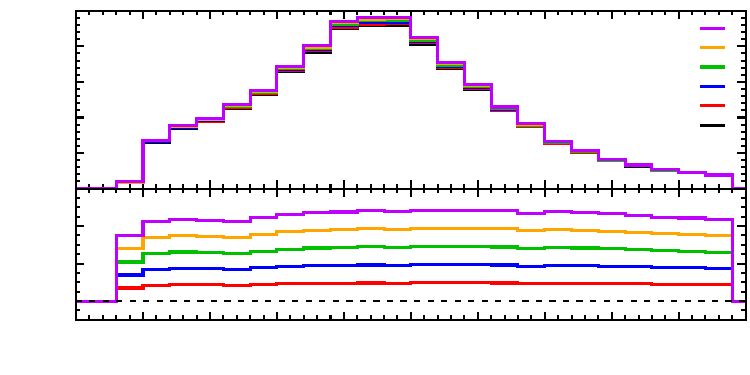
\includegraphics{nuenorm_E_FHC_sys0}}%
    \gplfronttext
  \end{picture}%
\endgroup
}
	\hfill
	\resizebox{0.475\linewidth}{!}{% GNUPLOT: LaTeX picture with Postscript
\begingroup
  \makeatletter
  \providecommand\color[2][]{%
    \GenericError{(gnuplot) \space\space\space\@spaces}{%
      Package color not loaded in conjunction with
      terminal option `colourtext'%
    }{See the gnuplot documentation for explanation.%
    }{Either use 'blacktext' in gnuplot or load the package
      color.sty in LaTeX.}%
    \renewcommand\color[2][]{}%
  }%
  \providecommand\includegraphics[2][]{%
    \GenericError{(gnuplot) \space\space\space\@spaces}{%
      Package graphicx or graphics not loaded%
    }{See the gnuplot documentation for explanation.%
    }{The gnuplot epslatex terminal needs graphicx.sty or graphics.sty.}%
    \renewcommand\includegraphics[2][]{}%
  }%
  \providecommand\rotatebox[2]{#2}%
  \@ifundefined{ifGPcolor}{%
    \newif\ifGPcolor
    \GPcolortrue
  }{}%
  \@ifundefined{ifGPblacktext}{%
    \newif\ifGPblacktext
    \GPblacktexttrue
  }{}%
  % define a \g@addto@macro without @ in the name:
  \let\gplgaddtomacro\g@addto@macro
  % define empty templates for all commands taking text:
  \gdef\gplbacktext{}%
  \gdef\gplfronttext{}%
  \makeatother
  \ifGPblacktext
    % no textcolor at all
    \def\colorrgb#1{}%
    \def\colorgray#1{}%
  \else
    % gray or color?
    \ifGPcolor
      \def\colorrgb#1{\color[rgb]{#1}}%
      \def\colorgray#1{\color[gray]{#1}}%
      \expandafter\def\csname LTw\endcsname{\color{white}}%
      \expandafter\def\csname LTb\endcsname{\color{black}}%
      \expandafter\def\csname LTa\endcsname{\color{black}}%
      \expandafter\def\csname LT0\endcsname{\color[rgb]{1,0,0}}%
      \expandafter\def\csname LT1\endcsname{\color[rgb]{0,1,0}}%
      \expandafter\def\csname LT2\endcsname{\color[rgb]{0,0,1}}%
      \expandafter\def\csname LT3\endcsname{\color[rgb]{1,0,1}}%
      \expandafter\def\csname LT4\endcsname{\color[rgb]{0,1,1}}%
      \expandafter\def\csname LT5\endcsname{\color[rgb]{1,1,0}}%
      \expandafter\def\csname LT6\endcsname{\color[rgb]{0,0,0}}%
      \expandafter\def\csname LT7\endcsname{\color[rgb]{1,0.3,0}}%
      \expandafter\def\csname LT8\endcsname{\color[rgb]{0.5,0.5,0.5}}%
    \else
      % gray
      \def\colorrgb#1{\color{black}}%
      \def\colorgray#1{\color[gray]{#1}}%
      \expandafter\def\csname LTw\endcsname{\color{white}}%
      \expandafter\def\csname LTb\endcsname{\color{black}}%
      \expandafter\def\csname LTa\endcsname{\color{black}}%
      \expandafter\def\csname LT0\endcsname{\color{black}}%
      \expandafter\def\csname LT1\endcsname{\color{black}}%
      \expandafter\def\csname LT2\endcsname{\color{black}}%
      \expandafter\def\csname LT3\endcsname{\color{black}}%
      \expandafter\def\csname LT4\endcsname{\color{black}}%
      \expandafter\def\csname LT5\endcsname{\color{black}}%
      \expandafter\def\csname LT6\endcsname{\color{black}}%
      \expandafter\def\csname LT7\endcsname{\color{black}}%
      \expandafter\def\csname LT8\endcsname{\color{black}}%
    \fi
  \fi
    \setlength{\unitlength}{0.0500bp}%
    \ifx\gptboxheight\undefined%
      \newlength{\gptboxheight}%
      \newlength{\gptboxwidth}%
      \newsavebox{\gptboxtext}%
    \fi%
    \setlength{\fboxrule}{0.5pt}%
    \setlength{\fboxsep}{1pt}%
\begin{picture}(7200.00,3600.00)%
    \gplgaddtomacro\gplbacktext{%
      \csname LTb\endcsname%%
      \put(618,540){\makebox(0,0)[r]{\strut{}0.99}}%
      \csname LTb\endcsname%%
      \put(618,855){\makebox(0,0)[r]{\strut{}1}}%
      \csname LTb\endcsname%%
      \put(618,1170){\makebox(0,0)[r]{\strut{}1.01}}%
      \csname LTb\endcsname%%
      \put(618,1485){\makebox(0,0)[r]{\strut{}1.02}}%
      \csname LTb\endcsname%%
      \put(720,354){\makebox(0,0){\strut{}0}}%
      \csname LTb\endcsname%%
      \put(1363,354){\makebox(0,0){\strut{}0.125}}%
      \csname LTb\endcsname%%
      \put(2006,354){\makebox(0,0){\strut{}0.25}}%
      \csname LTb\endcsname%%
      \put(2648,354){\makebox(0,0){\strut{}0.375}}%
      \csname LTb\endcsname%%
      \put(3291,354){\makebox(0,0){\strut{}0.5}}%
      \csname LTb\endcsname%%
      \put(3934,354){\makebox(0,0){\strut{}0.625}}%
      \csname LTb\endcsname%%
      \put(4577,354){\makebox(0,0){\strut{}0.75}}%
      \csname LTb\endcsname%%
      \put(5220,354){\makebox(0,0){\strut{}0.875}}%
      \csname LTb\endcsname%%
      \put(5862,354){\makebox(0,0){\strut{}1}}%
      \csname LTb\endcsname%%
      \put(6505,354){\makebox(0,0){\strut{}1.125}}%
      \csname LTb\endcsname%%
      \put(7148,354){\makebox(0,0){\strut{}1.25}}%
    }%
    \gplgaddtomacro\gplfronttext{%
      \csname LTb\endcsname%%
      \put(24,1170){\rotatebox{-270}{\makebox(0,0){\strut{}$1\sigma$ histogram}}}%
      \csname LTb\endcsname%%
      \put(3934,75){\makebox(0,0){\strut{}Energy (GeV)}}%
    }%
    \gplgaddtomacro\gplbacktext{%
      \csname LTb\endcsname%%
      \put(618,1800){\makebox(0,0)[r]{\strut{}0}}%
      \csname LTb\endcsname%%
      \put(618,2227){\makebox(0,0)[r]{\strut{}50}}%
      \csname LTb\endcsname%%
      \put(618,2653){\makebox(0,0)[r]{\strut{}100}}%
      \csname LTb\endcsname%%
      \put(618,3080){\makebox(0,0)[r]{\strut{}150}}%
      \csname LTb\endcsname%%
      \put(618,3506){\makebox(0,0)[r]{\strut{}200}}%
      \csname LTb\endcsname%%
      \put(720,1614){\makebox(0,0){\strut{}}}%
      \csname LTb\endcsname%%
      \put(1363,1614){\makebox(0,0){\strut{}}}%
      \csname LTb\endcsname%%
      \put(2006,1614){\makebox(0,0){\strut{}}}%
      \csname LTb\endcsname%%
      \put(2648,1614){\makebox(0,0){\strut{}}}%
      \csname LTb\endcsname%%
      \put(3291,1614){\makebox(0,0){\strut{}}}%
      \csname LTb\endcsname%%
      \put(3934,1614){\makebox(0,0){\strut{}}}%
      \csname LTb\endcsname%%
      \put(4577,1614){\makebox(0,0){\strut{}}}%
      \csname LTb\endcsname%%
      \put(5220,1614){\makebox(0,0){\strut{}}}%
      \csname LTb\endcsname%%
      \put(5862,1614){\makebox(0,0){\strut{}}}%
      \csname LTb\endcsname%%
      \put(6505,1614){\makebox(0,0){\strut{}}}%
      \csname LTb\endcsname%%
      \put(7148,1614){\makebox(0,0){\strut{}}}%
    }%
    \gplgaddtomacro\gplfronttext{%
      \csname LTb\endcsname%%
      \put(126,2653){\rotatebox{-270}{\makebox(0,0){\strut{}Events}}}%
      \csname LTb\endcsname%%
      \put(3934,1558){\makebox(0,0){\strut{}}}%
      \csname LTb\endcsname%%
      \put(6009,2409){\makebox(0,0)[l]{\strut{}No syst}}%
      \csname LTb\endcsname%%
      \put(6309,2595){\makebox(0,0)[l]{\strut{}1\%}}%
      \csname LTb\endcsname%%
      \put(6309,2781){\makebox(0,0)[l]{\strut{}2\%}}%
      \csname LTb\endcsname%%
      \put(6309,2967){\makebox(0,0)[l]{\strut{}3\%}}%
      \csname LTb\endcsname%%
      \put(6309,3153){\makebox(0,0)[l]{\strut{}4\%}}%
      \csname LTb\endcsname%%
      \put(6309,3339){\makebox(0,0)[l]{\strut{}5\%}}%
    }%
    \gplbacktext
    \put(0,0){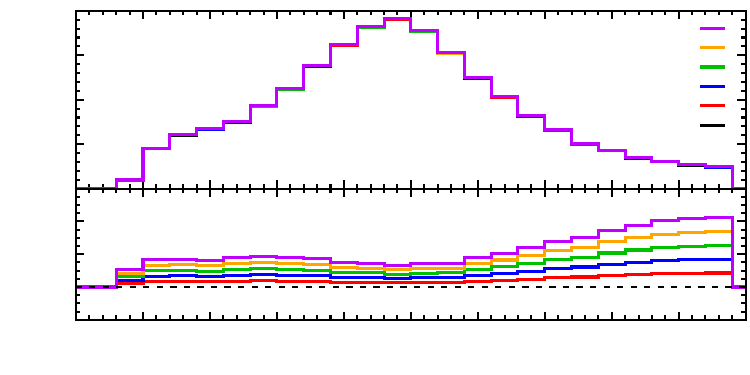
\includegraphics{nuenorm_E_RHC_sys0}}%
    \gplfronttext
  \end{picture}%
\endgroup
}

	\medskip
	\resizebox{0.475\linewidth}{!}{% GNUPLOT: LaTeX picture with Postscript
\begingroup
  \makeatletter
  \providecommand\color[2][]{%
    \GenericError{(gnuplot) \space\space\space\@spaces}{%
      Package color not loaded in conjunction with
      terminal option `colourtext'%
    }{See the gnuplot documentation for explanation.%
    }{Either use 'blacktext' in gnuplot or load the package
      color.sty in LaTeX.}%
    \renewcommand\color[2][]{}%
  }%
  \providecommand\includegraphics[2][]{%
    \GenericError{(gnuplot) \space\space\space\@spaces}{%
      Package graphicx or graphics not loaded%
    }{See the gnuplot documentation for explanation.%
    }{The gnuplot epslatex terminal needs graphicx.sty or graphics.sty.}%
    \renewcommand\includegraphics[2][]{}%
  }%
  \providecommand\rotatebox[2]{#2}%
  \@ifundefined{ifGPcolor}{%
    \newif\ifGPcolor
    \GPcolortrue
  }{}%
  \@ifundefined{ifGPblacktext}{%
    \newif\ifGPblacktext
    \GPblacktexttrue
  }{}%
  % define a \g@addto@macro without @ in the name:
  \let\gplgaddtomacro\g@addto@macro
  % define empty templates for all commands taking text:
  \gdef\gplbacktext{}%
  \gdef\gplfronttext{}%
  \makeatother
  \ifGPblacktext
    % no textcolor at all
    \def\colorrgb#1{}%
    \def\colorgray#1{}%
  \else
    % gray or color?
    \ifGPcolor
      \def\colorrgb#1{\color[rgb]{#1}}%
      \def\colorgray#1{\color[gray]{#1}}%
      \expandafter\def\csname LTw\endcsname{\color{white}}%
      \expandafter\def\csname LTb\endcsname{\color{black}}%
      \expandafter\def\csname LTa\endcsname{\color{black}}%
      \expandafter\def\csname LT0\endcsname{\color[rgb]{1,0,0}}%
      \expandafter\def\csname LT1\endcsname{\color[rgb]{0,1,0}}%
      \expandafter\def\csname LT2\endcsname{\color[rgb]{0,0,1}}%
      \expandafter\def\csname LT3\endcsname{\color[rgb]{1,0,1}}%
      \expandafter\def\csname LT4\endcsname{\color[rgb]{0,1,1}}%
      \expandafter\def\csname LT5\endcsname{\color[rgb]{1,1,0}}%
      \expandafter\def\csname LT6\endcsname{\color[rgb]{0,0,0}}%
      \expandafter\def\csname LT7\endcsname{\color[rgb]{1,0.3,0}}%
      \expandafter\def\csname LT8\endcsname{\color[rgb]{0.5,0.5,0.5}}%
    \else
      % gray
      \def\colorrgb#1{\color{black}}%
      \def\colorgray#1{\color[gray]{#1}}%
      \expandafter\def\csname LTw\endcsname{\color{white}}%
      \expandafter\def\csname LTb\endcsname{\color{black}}%
      \expandafter\def\csname LTa\endcsname{\color{black}}%
      \expandafter\def\csname LT0\endcsname{\color{black}}%
      \expandafter\def\csname LT1\endcsname{\color{black}}%
      \expandafter\def\csname LT2\endcsname{\color{black}}%
      \expandafter\def\csname LT3\endcsname{\color{black}}%
      \expandafter\def\csname LT4\endcsname{\color{black}}%
      \expandafter\def\csname LT5\endcsname{\color{black}}%
      \expandafter\def\csname LT6\endcsname{\color{black}}%
      \expandafter\def\csname LT7\endcsname{\color{black}}%
      \expandafter\def\csname LT8\endcsname{\color{black}}%
    \fi
  \fi
    \setlength{\unitlength}{0.0500bp}%
    \ifx\gptboxheight\undefined%
      \newlength{\gptboxheight}%
      \newlength{\gptboxwidth}%
      \newsavebox{\gptboxtext}%
    \fi%
    \setlength{\fboxrule}{0.5pt}%
    \setlength{\fboxsep}{1pt}%
\begin{picture}(7200.00,3600.00)%
    \gplgaddtomacro\gplbacktext{%
      \csname LTb\endcsname%%
      \put(618,792){\makebox(0,0)[r]{\strut{}1}}%
      \csname LTb\endcsname%%
      \put(618,1296){\makebox(0,0)[r]{\strut{}1.002}}%
      \csname LTb\endcsname%%
      \put(720,354){\makebox(0,0){\strut{}0}}%
      \csname LTb\endcsname%%
      \put(1363,354){\makebox(0,0){\strut{}0.125}}%
      \csname LTb\endcsname%%
      \put(2006,354){\makebox(0,0){\strut{}0.25}}%
      \csname LTb\endcsname%%
      \put(2648,354){\makebox(0,0){\strut{}0.375}}%
      \csname LTb\endcsname%%
      \put(3291,354){\makebox(0,0){\strut{}0.5}}%
      \csname LTb\endcsname%%
      \put(3934,354){\makebox(0,0){\strut{}0.625}}%
      \csname LTb\endcsname%%
      \put(4577,354){\makebox(0,0){\strut{}0.75}}%
      \csname LTb\endcsname%%
      \put(5220,354){\makebox(0,0){\strut{}0.875}}%
      \csname LTb\endcsname%%
      \put(5862,354){\makebox(0,0){\strut{}1}}%
      \csname LTb\endcsname%%
      \put(6505,354){\makebox(0,0){\strut{}1.125}}%
      \csname LTb\endcsname%%
      \put(7148,354){\makebox(0,0){\strut{}1.25}}%
    }%
    \gplgaddtomacro\gplfronttext{%
      \csname LTb\endcsname%%
      \put(3934,75){\makebox(0,0){\strut{}Energy (GeV)}}%
    }%
    \gplgaddtomacro\gplbacktext{%
      \csname LTb\endcsname%%
      \put(618,1800){\makebox(0,0)[r]{\strut{}0}}%
      \csname LTb\endcsname%%
      \put(618,2141){\makebox(0,0)[r]{\strut{}50}}%
      \csname LTb\endcsname%%
      \put(618,2482){\makebox(0,0)[r]{\strut{}100}}%
      \csname LTb\endcsname%%
      \put(618,2824){\makebox(0,0)[r]{\strut{}150}}%
      \csname LTb\endcsname%%
      \put(618,3165){\makebox(0,0)[r]{\strut{}200}}%
      \csname LTb\endcsname%%
      \put(618,3506){\makebox(0,0)[r]{\strut{}250}}%
      \csname LTb\endcsname%%
      \put(720,1614){\makebox(0,0){\strut{}}}%
      \csname LTb\endcsname%%
      \put(1363,1614){\makebox(0,0){\strut{}}}%
      \csname LTb\endcsname%%
      \put(2006,1614){\makebox(0,0){\strut{}}}%
      \csname LTb\endcsname%%
      \put(2648,1614){\makebox(0,0){\strut{}}}%
      \csname LTb\endcsname%%
      \put(3291,1614){\makebox(0,0){\strut{}}}%
      \csname LTb\endcsname%%
      \put(3934,1614){\makebox(0,0){\strut{}}}%
      \csname LTb\endcsname%%
      \put(4577,1614){\makebox(0,0){\strut{}}}%
      \csname LTb\endcsname%%
      \put(5220,1614){\makebox(0,0){\strut{}}}%
      \csname LTb\endcsname%%
      \put(5862,1614){\makebox(0,0){\strut{}}}%
      \csname LTb\endcsname%%
      \put(6505,1614){\makebox(0,0){\strut{}}}%
      \csname LTb\endcsname%%
      \put(7148,1614){\makebox(0,0){\strut{}}}%
    }%
    \gplgaddtomacro\gplfronttext{%
      \csname LTb\endcsname%%
      \put(126,2653){\rotatebox{-270}{\makebox(0,0){\strut{}Events}}}%
      \csname LTb\endcsname%%
      \put(3934,1558){\makebox(0,0){\strut{}}}%
      \csname LTb\endcsname%%
      \put(6009,2409){\makebox(0,0)[l]{\strut{}No syst}}%
      \csname LTb\endcsname%%
      \put(6309,2595){\makebox(0,0)[l]{\strut{}1\%}}%
      \csname LTb\endcsname%%
      \put(6309,2781){\makebox(0,0)[l]{\strut{}2\%}}%
      \csname LTb\endcsname%%
      \put(6309,2967){\makebox(0,0)[l]{\strut{}3\%}}%
      \csname LTb\endcsname%%
      \put(6309,3153){\makebox(0,0)[l]{\strut{}4\%}}%
      \csname LTb\endcsname%%
      \put(6309,3339){\makebox(0,0)[l]{\strut{}5\%}}%
    }%
    \gplbacktext
    \put(0,0){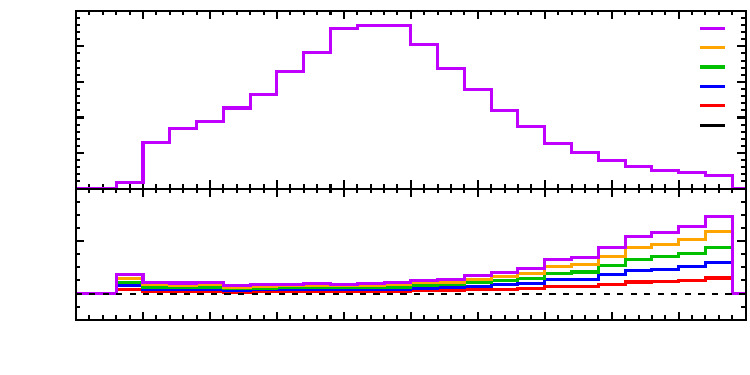
\includegraphics{nuenorm_E_FHC_sys1}}%
    \gplfronttext
  \end{picture}%
\endgroup
}
	\hfill
	\resizebox{0.475\linewidth}{!}{% GNUPLOT: LaTeX picture with Postscript
\begingroup
  \makeatletter
  \providecommand\color[2][]{%
    \GenericError{(gnuplot) \space\space\space\@spaces}{%
      Package color not loaded in conjunction with
      terminal option `colourtext'%
    }{See the gnuplot documentation for explanation.%
    }{Either use 'blacktext' in gnuplot or load the package
      color.sty in LaTeX.}%
    \renewcommand\color[2][]{}%
  }%
  \providecommand\includegraphics[2][]{%
    \GenericError{(gnuplot) \space\space\space\@spaces}{%
      Package graphicx or graphics not loaded%
    }{See the gnuplot documentation for explanation.%
    }{The gnuplot epslatex terminal needs graphicx.sty or graphics.sty.}%
    \renewcommand\includegraphics[2][]{}%
  }%
  \providecommand\rotatebox[2]{#2}%
  \@ifundefined{ifGPcolor}{%
    \newif\ifGPcolor
    \GPcolortrue
  }{}%
  \@ifundefined{ifGPblacktext}{%
    \newif\ifGPblacktext
    \GPblacktexttrue
  }{}%
  % define a \g@addto@macro without @ in the name:
  \let\gplgaddtomacro\g@addto@macro
  % define empty templates for all commands taking text:
  \gdef\gplbacktext{}%
  \gdef\gplfronttext{}%
  \makeatother
  \ifGPblacktext
    % no textcolor at all
    \def\colorrgb#1{}%
    \def\colorgray#1{}%
  \else
    % gray or color?
    \ifGPcolor
      \def\colorrgb#1{\color[rgb]{#1}}%
      \def\colorgray#1{\color[gray]{#1}}%
      \expandafter\def\csname LTw\endcsname{\color{white}}%
      \expandafter\def\csname LTb\endcsname{\color{black}}%
      \expandafter\def\csname LTa\endcsname{\color{black}}%
      \expandafter\def\csname LT0\endcsname{\color[rgb]{1,0,0}}%
      \expandafter\def\csname LT1\endcsname{\color[rgb]{0,1,0}}%
      \expandafter\def\csname LT2\endcsname{\color[rgb]{0,0,1}}%
      \expandafter\def\csname LT3\endcsname{\color[rgb]{1,0,1}}%
      \expandafter\def\csname LT4\endcsname{\color[rgb]{0,1,1}}%
      \expandafter\def\csname LT5\endcsname{\color[rgb]{1,1,0}}%
      \expandafter\def\csname LT6\endcsname{\color[rgb]{0,0,0}}%
      \expandafter\def\csname LT7\endcsname{\color[rgb]{1,0.3,0}}%
      \expandafter\def\csname LT8\endcsname{\color[rgb]{0.5,0.5,0.5}}%
    \else
      % gray
      \def\colorrgb#1{\color{black}}%
      \def\colorgray#1{\color[gray]{#1}}%
      \expandafter\def\csname LTw\endcsname{\color{white}}%
      \expandafter\def\csname LTb\endcsname{\color{black}}%
      \expandafter\def\csname LTa\endcsname{\color{black}}%
      \expandafter\def\csname LT0\endcsname{\color{black}}%
      \expandafter\def\csname LT1\endcsname{\color{black}}%
      \expandafter\def\csname LT2\endcsname{\color{black}}%
      \expandafter\def\csname LT3\endcsname{\color{black}}%
      \expandafter\def\csname LT4\endcsname{\color{black}}%
      \expandafter\def\csname LT5\endcsname{\color{black}}%
      \expandafter\def\csname LT6\endcsname{\color{black}}%
      \expandafter\def\csname LT7\endcsname{\color{black}}%
      \expandafter\def\csname LT8\endcsname{\color{black}}%
    \fi
  \fi
    \setlength{\unitlength}{0.0500bp}%
    \ifx\gptboxheight\undefined%
      \newlength{\gptboxheight}%
      \newlength{\gptboxwidth}%
      \newsavebox{\gptboxtext}%
    \fi%
    \setlength{\fboxrule}{0.5pt}%
    \setlength{\fboxsep}{1pt}%
\begin{picture}(7200.00,3600.00)%
    \gplgaddtomacro\gplbacktext{%
      \csname LTb\endcsname%%
      \put(618,750){\makebox(0,0)[r]{\strut{}1}}%
      \csname LTb\endcsname%%
      \put(618,1170){\makebox(0,0)[r]{\strut{}1.02}}%
      \csname LTb\endcsname%%
      \put(618,1590){\makebox(0,0)[r]{\strut{}1.04}}%
      \csname LTb\endcsname%%
      \put(720,354){\makebox(0,0){\strut{}0}}%
      \csname LTb\endcsname%%
      \put(1363,354){\makebox(0,0){\strut{}0.125}}%
      \csname LTb\endcsname%%
      \put(2006,354){\makebox(0,0){\strut{}0.25}}%
      \csname LTb\endcsname%%
      \put(2648,354){\makebox(0,0){\strut{}0.375}}%
      \csname LTb\endcsname%%
      \put(3291,354){\makebox(0,0){\strut{}0.5}}%
      \csname LTb\endcsname%%
      \put(3934,354){\makebox(0,0){\strut{}0.625}}%
      \csname LTb\endcsname%%
      \put(4577,354){\makebox(0,0){\strut{}0.75}}%
      \csname LTb\endcsname%%
      \put(5220,354){\makebox(0,0){\strut{}0.875}}%
      \csname LTb\endcsname%%
      \put(5862,354){\makebox(0,0){\strut{}1}}%
      \csname LTb\endcsname%%
      \put(6505,354){\makebox(0,0){\strut{}1.125}}%
      \csname LTb\endcsname%%
      \put(7148,354){\makebox(0,0){\strut{}1.25}}%
    }%
    \gplgaddtomacro\gplfronttext{%
      \csname LTb\endcsname%%
      \put(24,1170){\rotatebox{-270}{\makebox(0,0){\strut{}$1\sigma$ histogram}}}%
      \csname LTb\endcsname%%
      \put(3934,75){\makebox(0,0){\strut{}Energy (GeV)}}%
    }%
    \gplgaddtomacro\gplbacktext{%
      \csname LTb\endcsname%%
      \put(618,1800){\makebox(0,0)[r]{\strut{}0}}%
      \csname LTb\endcsname%%
      \put(618,2227){\makebox(0,0)[r]{\strut{}50}}%
      \csname LTb\endcsname%%
      \put(618,2653){\makebox(0,0)[r]{\strut{}100}}%
      \csname LTb\endcsname%%
      \put(618,3080){\makebox(0,0)[r]{\strut{}150}}%
      \csname LTb\endcsname%%
      \put(618,3506){\makebox(0,0)[r]{\strut{}200}}%
      \csname LTb\endcsname%%
      \put(720,1614){\makebox(0,0){\strut{}}}%
      \csname LTb\endcsname%%
      \put(1363,1614){\makebox(0,0){\strut{}}}%
      \csname LTb\endcsname%%
      \put(2006,1614){\makebox(0,0){\strut{}}}%
      \csname LTb\endcsname%%
      \put(2648,1614){\makebox(0,0){\strut{}}}%
      \csname LTb\endcsname%%
      \put(3291,1614){\makebox(0,0){\strut{}}}%
      \csname LTb\endcsname%%
      \put(3934,1614){\makebox(0,0){\strut{}}}%
      \csname LTb\endcsname%%
      \put(4577,1614){\makebox(0,0){\strut{}}}%
      \csname LTb\endcsname%%
      \put(5220,1614){\makebox(0,0){\strut{}}}%
      \csname LTb\endcsname%%
      \put(5862,1614){\makebox(0,0){\strut{}}}%
      \csname LTb\endcsname%%
      \put(6505,1614){\makebox(0,0){\strut{}}}%
      \csname LTb\endcsname%%
      \put(7148,1614){\makebox(0,0){\strut{}}}%
    }%
    \gplgaddtomacro\gplfronttext{%
      \csname LTb\endcsname%%
      \put(126,2653){\rotatebox{-270}{\makebox(0,0){\strut{}Events}}}%
      \csname LTb\endcsname%%
      \put(3934,1558){\makebox(0,0){\strut{}}}%
      \csname LTb\endcsname%%
      \put(6009,2409){\makebox(0,0)[l]{\strut{}No syst}}%
      \csname LTb\endcsname%%
      \put(6309,2595){\makebox(0,0)[l]{\strut{}1\%}}%
      \csname LTb\endcsname%%
      \put(6309,2781){\makebox(0,0)[l]{\strut{}2\%}}%
      \csname LTb\endcsname%%
      \put(6309,2967){\makebox(0,0)[l]{\strut{}3\%}}%
      \csname LTb\endcsname%%
      \put(6309,3153){\makebox(0,0)[l]{\strut{}4\%}}%
      \csname LTb\endcsname%%
      \put(6309,3339){\makebox(0,0)[l]{\strut{}5\%}}%
    }%
    \gplbacktext
    \put(0,0){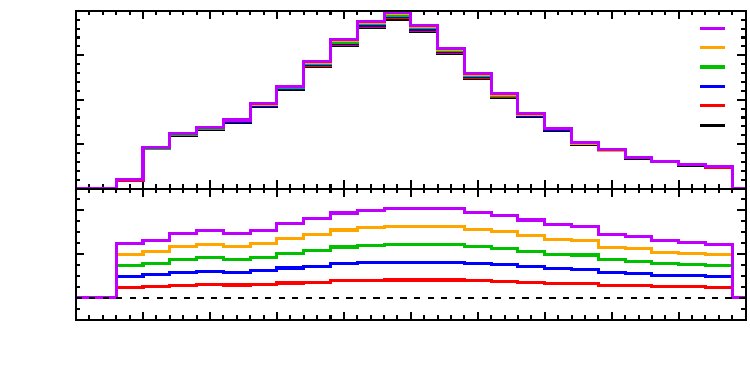
\includegraphics{nuenorm_E_RHC_sys1}}%
    \gplfronttext
  \end{picture}%
\endgroup
}
	\caption{Prediction of events at the far detector for the one ring $e$-like sample in %
		$\nu$-mode (left) and $\cj{\nu}$-mode (right).
		The $\nu_e$ (top) and $\cj{\nu}_e$ (bottom) CC cross-section systematics are varied to reach relative errors %
		between 1,\% and 5\,\%.
		In each figure, the top panel shows how the event distribution is affected, and the bottom panel shows %
		the variation with respect to the prediction without errors applied, which is by definition %
		the $1\sigma$ histogram, $1 + f^n$ (see \refeq{eq:chi2}). }
	\label{fig:nuenorm_prediction}
\end{figure}

\begin{figure}
	\centering
	\resizebox{0.48\linewidth}{!}{% GNUPLOT: LaTeX picture with Postscript
\begingroup
  \makeatletter
  \providecommand\color[2][]{%
    \GenericError{(gnuplot) \space\space\space\@spaces}{%
      Package color not loaded in conjunction with
      terminal option `colourtext'%
    }{See the gnuplot documentation for explanation.%
    }{Either use 'blacktext' in gnuplot or load the package
      color.sty in LaTeX.}%
    \renewcommand\color[2][]{}%
  }%
  \providecommand\includegraphics[2][]{%
    \GenericError{(gnuplot) \space\space\space\@spaces}{%
      Package graphicx or graphics not loaded%
    }{See the gnuplot documentation for explanation.%
    }{The gnuplot epslatex terminal needs graphicx.sty or graphics.sty.}%
    \renewcommand\includegraphics[2][]{}%
  }%
  \providecommand\rotatebox[2]{#2}%
  \@ifundefined{ifGPcolor}{%
    \newif\ifGPcolor
    \GPcolortrue
  }{}%
  \@ifundefined{ifGPblacktext}{%
    \newif\ifGPblacktext
    \GPblacktexttrue
  }{}%
  % define a \g@addto@macro without @ in the name:
  \let\gplgaddtomacro\g@addto@macro
  % define empty templates for all commands taking text:
  \gdef\gplbacktext{}%
  \gdef\gplfronttext{}%
  \makeatother
  \ifGPblacktext
    % no textcolor at all
    \def\colorrgb#1{}%
    \def\colorgray#1{}%
  \else
    % gray or color?
    \ifGPcolor
      \def\colorrgb#1{\color[rgb]{#1}}%
      \def\colorgray#1{\color[gray]{#1}}%
      \expandafter\def\csname LTw\endcsname{\color{white}}%
      \expandafter\def\csname LTb\endcsname{\color{black}}%
      \expandafter\def\csname LTa\endcsname{\color{black}}%
      \expandafter\def\csname LT0\endcsname{\color[rgb]{1,0,0}}%
      \expandafter\def\csname LT1\endcsname{\color[rgb]{0,1,0}}%
      \expandafter\def\csname LT2\endcsname{\color[rgb]{0,0,1}}%
      \expandafter\def\csname LT3\endcsname{\color[rgb]{1,0,1}}%
      \expandafter\def\csname LT4\endcsname{\color[rgb]{0,1,1}}%
      \expandafter\def\csname LT5\endcsname{\color[rgb]{1,1,0}}%
      \expandafter\def\csname LT6\endcsname{\color[rgb]{0,0,0}}%
      \expandafter\def\csname LT7\endcsname{\color[rgb]{1,0.3,0}}%
      \expandafter\def\csname LT8\endcsname{\color[rgb]{0.5,0.5,0.5}}%
    \else
      % gray
      \def\colorrgb#1{\color{black}}%
      \def\colorgray#1{\color[gray]{#1}}%
      \expandafter\def\csname LTw\endcsname{\color{white}}%
      \expandafter\def\csname LTb\endcsname{\color{black}}%
      \expandafter\def\csname LTa\endcsname{\color{black}}%
      \expandafter\def\csname LT0\endcsname{\color{black}}%
      \expandafter\def\csname LT1\endcsname{\color{black}}%
      \expandafter\def\csname LT2\endcsname{\color{black}}%
      \expandafter\def\csname LT3\endcsname{\color{black}}%
      \expandafter\def\csname LT4\endcsname{\color{black}}%
      \expandafter\def\csname LT5\endcsname{\color{black}}%
      \expandafter\def\csname LT6\endcsname{\color{black}}%
      \expandafter\def\csname LT7\endcsname{\color{black}}%
      \expandafter\def\csname LT8\endcsname{\color{black}}%
    \fi
  \fi
    \setlength{\unitlength}{0.0500bp}%
    \ifx\gptboxheight\undefined%
      \newlength{\gptboxheight}%
      \newlength{\gptboxwidth}%
      \newsavebox{\gptboxtext}%
    \fi%
    \setlength{\fboxrule}{0.5pt}%
    \setlength{\fboxsep}{1pt}%
\begin{picture}(10800.00,7560.00)%
    \gplgaddtomacro\gplbacktext{%
      \csname LTb\endcsname%%
      \put(870,680){\makebox(0,0)[r]{\strut{}-1}}%
      \csname LTb\endcsname%%
      \put(870,1123){\makebox(0,0)[r]{\strut{}0}}%
      \csname LTb\endcsname%%
      \put(870,1566){\makebox(0,0)[r]{\strut{}1}}%
      \csname LTb\endcsname%%
      \put(870,2009){\makebox(0,0)[r]{\strut{}2}}%
      \csname LTb\endcsname%%
      \put(870,2451){\makebox(0,0)[r]{\strut{}3}}%
      \csname LTb\endcsname%%
      \put(870,2894){\makebox(0,0)[r]{\strut{}4}}%
      \csname LTb\endcsname%%
      \put(870,3337){\makebox(0,0)[r]{\strut{}5}}%
      \csname LTb\endcsname%%
      \put(972,494){\makebox(0,0){\strut{}-1.00$\pi$}}%
      \csname LTb\endcsname%%
      \put(1934,494){\makebox(0,0){\strut{}-0.80$\pi$}}%
      \csname LTb\endcsname%%
      \put(2897,494){\makebox(0,0){\strut{}-0.60$\pi$}}%
      \csname LTb\endcsname%%
      \put(3859,494){\makebox(0,0){\strut{}-0.40$\pi$}}%
      \csname LTb\endcsname%%
      \put(4821,494){\makebox(0,0){\strut{}-0.20$\pi$}}%
      \csname LTb\endcsname%%
      \put(5784,494){\makebox(0,0){\strut{}0.00$\pi$}}%
      \csname LTb\endcsname%%
      \put(6746,494){\makebox(0,0){\strut{}0.20$\pi$}}%
      \csname LTb\endcsname%%
      \put(7708,494){\makebox(0,0){\strut{}0.40$\pi$}}%
      \csname LTb\endcsname%%
      \put(8670,494){\makebox(0,0){\strut{}0.60$\pi$}}%
      \csname LTb\endcsname%%
      \put(9633,494){\makebox(0,0){\strut{}0.80$\pi$}}%
      \csname LTb\endcsname%%
      \put(10595,494){\makebox(0,0){\strut{}1.00$\pi$}}%
    }%
    \gplgaddtomacro\gplfronttext{%
      \csname LTb\endcsname%%
      \put(480,2230){\rotatebox{-270}{\makebox(0,0){\strut{}$\Delta \chi^2 - \Delta \chi^2_0$}}}%
      \csname LTb\endcsname%%
      \put(5783,215){\makebox(0,0){\strut{}$\delta_\text{CP}$}}%
      \csname LTb\endcsname%%
      \put(4231,2358){\makebox(0,0){\strut{}Difference}}%
      \csname LTb\endcsname%%
      \put(3758,2172){\makebox(0,0)[l]{\strut{}$1\%$}}%
      \csname LTb\endcsname%%
      \put(3758,1986){\makebox(0,0)[l]{\strut{}$2\%$}}%
      \csname LTb\endcsname%%
      \put(3758,1800){\makebox(0,0)[l]{\strut{}$3\%$}}%
      \csname LTb\endcsname%%
      \put(3758,1614){\makebox(0,0)[l]{\strut{}$4\%$}}%
      \csname LTb\endcsname%%
      \put(3758,1428){\makebox(0,0)[l]{\strut{}$5\%$}}%
    }%
    \gplgaddtomacro\gplbacktext{%
      \csname LTb\endcsname%%
      \put(870,3780){\makebox(0,0)[r]{\strut{}0}}%
      \csname LTb\endcsname%%
      \put(870,4149){\makebox(0,0)[r]{\strut{}50}}%
      \csname LTb\endcsname%%
      \put(870,4517){\makebox(0,0)[r]{\strut{}100}}%
      \csname LTb\endcsname%%
      \put(870,4886){\makebox(0,0)[r]{\strut{}150}}%
      \csname LTb\endcsname%%
      \put(870,5254){\makebox(0,0)[r]{\strut{}200}}%
      \csname LTb\endcsname%%
      \put(870,5623){\makebox(0,0)[r]{\strut{}250}}%
      \csname LTb\endcsname%%
      \put(870,5992){\makebox(0,0)[r]{\strut{}300}}%
      \csname LTb\endcsname%%
      \put(870,6360){\makebox(0,0)[r]{\strut{}350}}%
      \csname LTb\endcsname%%
      \put(870,6729){\makebox(0,0)[r]{\strut{}400}}%
      \csname LTb\endcsname%%
      \put(870,7097){\makebox(0,0)[r]{\strut{}450}}%
      \csname LTb\endcsname%%
      \put(870,7466){\makebox(0,0)[r]{\strut{}500}}%
      \csname LTb\endcsname%%
      \put(972,3594){\makebox(0,0){\strut{}}}%
      \csname LTb\endcsname%%
      \put(1934,3594){\makebox(0,0){\strut{}}}%
      \csname LTb\endcsname%%
      \put(2897,3594){\makebox(0,0){\strut{}}}%
      \csname LTb\endcsname%%
      \put(3859,3594){\makebox(0,0){\strut{}}}%
      \csname LTb\endcsname%%
      \put(4821,3594){\makebox(0,0){\strut{}}}%
      \csname LTb\endcsname%%
      \put(5784,3594){\makebox(0,0){\strut{}}}%
      \csname LTb\endcsname%%
      \put(6746,3594){\makebox(0,0){\strut{}}}%
      \csname LTb\endcsname%%
      \put(7708,3594){\makebox(0,0){\strut{}}}%
      \csname LTb\endcsname%%
      \put(8670,3594){\makebox(0,0){\strut{}}}%
      \csname LTb\endcsname%%
      \put(9633,3594){\makebox(0,0){\strut{}}}%
      \csname LTb\endcsname%%
      \put(10595,3594){\makebox(0,0){\strut{}}}%
    }%
    \gplgaddtomacro\gplfronttext{%
      \csname LTb\endcsname%%
      \put(378,5623){\rotatebox{-270}{\makebox(0,0){\strut{}$\Delta \chi^2$}}}%
      \csname LTb\endcsname%%
      \put(5783,3538){\makebox(0,0){\strut{}}}%
      \csname LTb\endcsname%%
      \put(4231,7004){\makebox(0,0){\strut{}}}%
      \csname LTb\endcsname%%
      \put(3758,7004){\makebox(0,0)[l]{\strut{}No syst}}%
      \csname LTb\endcsname%%
      \put(3758,6818){\makebox(0,0)[l]{\strut{}$1\%$}}%
      \csname LTb\endcsname%%
      \put(3758,6632){\makebox(0,0)[l]{\strut{}$2\%$}}%
      \csname LTb\endcsname%%
      \put(3758,6446){\makebox(0,0)[l]{\strut{}$3\%$}}%
      \csname LTb\endcsname%%
      \put(3758,6260){\makebox(0,0)[l]{\strut{}$4\%$}}%
      \csname LTb\endcsname%%
      \put(3758,6074){\makebox(0,0)[l]{\strut{}$5\%$}}%
    }%
    \gplbacktext
    \put(0,0){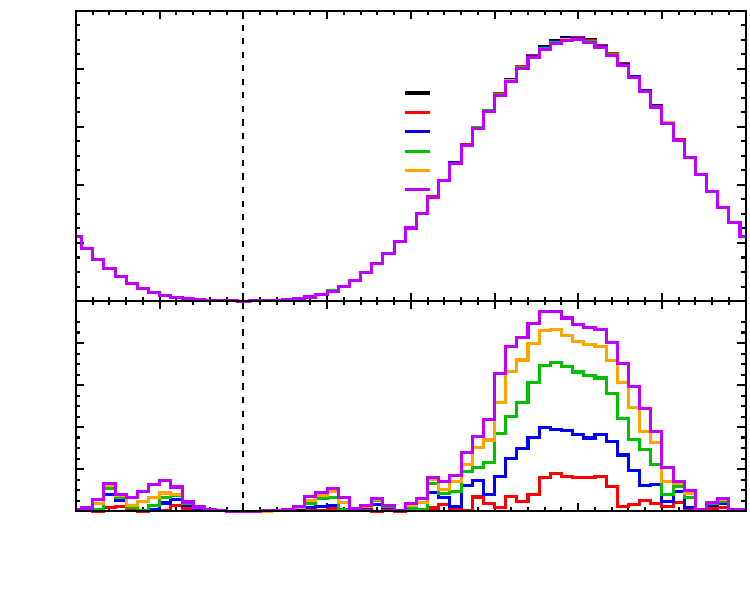
\includegraphics{pics/nuenorm_corr_chi2_dCP}}%
    \gplfronttext
  \end{picture}%
\endgroup
}
	\resizebox{0.48\linewidth}{!}{% GNUPLOT: LaTeX picture with Postscript
\begingroup
  \makeatletter
  \providecommand\color[2][]{%
    \GenericError{(gnuplot) \space\space\space\@spaces}{%
      Package color not loaded in conjunction with
      terminal option `colourtext'%
    }{See the gnuplot documentation for explanation.%
    }{Either use 'blacktext' in gnuplot or load the package
      color.sty in LaTeX.}%
    \renewcommand\color[2][]{}%
  }%
  \providecommand\includegraphics[2][]{%
    \GenericError{(gnuplot) \space\space\space\@spaces}{%
      Package graphicx or graphics not loaded%
    }{See the gnuplot documentation for explanation.%
    }{The gnuplot epslatex terminal needs graphicx.sty or graphics.sty.}%
    \renewcommand\includegraphics[2][]{}%
  }%
  \providecommand\rotatebox[2]{#2}%
  \@ifundefined{ifGPcolor}{%
    \newif\ifGPcolor
    \GPcolortrue
  }{}%
  \@ifundefined{ifGPblacktext}{%
    \newif\ifGPblacktext
    \GPblacktexttrue
  }{}%
  % define a \g@addto@macro without @ in the name:
  \let\gplgaddtomacro\g@addto@macro
  % define empty templates for all commands taking text:
  \gdef\gplbacktext{}%
  \gdef\gplfronttext{}%
  \makeatother
  \ifGPblacktext
    % no textcolor at all
    \def\colorrgb#1{}%
    \def\colorgray#1{}%
  \else
    % gray or color?
    \ifGPcolor
      \def\colorrgb#1{\color[rgb]{#1}}%
      \def\colorgray#1{\color[gray]{#1}}%
      \expandafter\def\csname LTw\endcsname{\color{white}}%
      \expandafter\def\csname LTb\endcsname{\color{black}}%
      \expandafter\def\csname LTa\endcsname{\color{black}}%
      \expandafter\def\csname LT0\endcsname{\color[rgb]{1,0,0}}%
      \expandafter\def\csname LT1\endcsname{\color[rgb]{0,1,0}}%
      \expandafter\def\csname LT2\endcsname{\color[rgb]{0,0,1}}%
      \expandafter\def\csname LT3\endcsname{\color[rgb]{1,0,1}}%
      \expandafter\def\csname LT4\endcsname{\color[rgb]{0,1,1}}%
      \expandafter\def\csname LT5\endcsname{\color[rgb]{1,1,0}}%
      \expandafter\def\csname LT6\endcsname{\color[rgb]{0,0,0}}%
      \expandafter\def\csname LT7\endcsname{\color[rgb]{1,0.3,0}}%
      \expandafter\def\csname LT8\endcsname{\color[rgb]{0.5,0.5,0.5}}%
    \else
      % gray
      \def\colorrgb#1{\color{black}}%
      \def\colorgray#1{\color[gray]{#1}}%
      \expandafter\def\csname LTw\endcsname{\color{white}}%
      \expandafter\def\csname LTb\endcsname{\color{black}}%
      \expandafter\def\csname LTa\endcsname{\color{black}}%
      \expandafter\def\csname LT0\endcsname{\color{black}}%
      \expandafter\def\csname LT1\endcsname{\color{black}}%
      \expandafter\def\csname LT2\endcsname{\color{black}}%
      \expandafter\def\csname LT3\endcsname{\color{black}}%
      \expandafter\def\csname LT4\endcsname{\color{black}}%
      \expandafter\def\csname LT5\endcsname{\color{black}}%
      \expandafter\def\csname LT6\endcsname{\color{black}}%
      \expandafter\def\csname LT7\endcsname{\color{black}}%
      \expandafter\def\csname LT8\endcsname{\color{black}}%
    \fi
  \fi
    \setlength{\unitlength}{0.0500bp}%
    \ifx\gptboxheight\undefined%
      \newlength{\gptboxheight}%
      \newlength{\gptboxwidth}%
      \newsavebox{\gptboxtext}%
    \fi%
    \setlength{\fboxrule}{0.5pt}%
    \setlength{\fboxsep}{1pt}%
\begin{picture}(7200.00,5760.00)%
    \gplgaddtomacro\gplbacktext{%
      \csname LTb\endcsname%%
      \put(618,864){\makebox(0,0)[r]{\strut{}0}}%
      \csname LTb\endcsname%%
      \put(618,1368){\makebox(0,0)[r]{\strut{}100}}%
      \csname LTb\endcsname%%
      \put(618,1872){\makebox(0,0)[r]{\strut{}200}}%
      \csname LTb\endcsname%%
      \put(618,2376){\makebox(0,0)[r]{\strut{}300}}%
      \csname LTb\endcsname%%
      \put(720,678){\makebox(0,0){\strut{}-1.00$\pi$}}%
      \csname LTb\endcsname%%
      \put(1524,678){\makebox(0,0){\strut{}-0.75$\pi$}}%
      \csname LTb\endcsname%%
      \put(2327,678){\makebox(0,0){\strut{}-0.50$\pi$}}%
      \csname LTb\endcsname%%
      \put(3131,678){\makebox(0,0){\strut{}-0.25$\pi$}}%
      \csname LTb\endcsname%%
      \put(3934,678){\makebox(0,0){\strut{}0.00$\pi$}}%
      \csname LTb\endcsname%%
      \put(4738,678){\makebox(0,0){\strut{}0.25$\pi$}}%
      \csname LTb\endcsname%%
      \put(5541,678){\makebox(0,0){\strut{}0.50$\pi$}}%
      \csname LTb\endcsname%%
      \put(6345,678){\makebox(0,0){\strut{}0.75$\pi$}}%
      \csname LTb\endcsname%%
      \put(7148,678){\makebox(0,0){\strut{}1.00$\pi$}}%
    }%
    \gplgaddtomacro\gplfronttext{%
      \csname LTb\endcsname%%
      \put(126,1872){\rotatebox{-270}{\makebox(0,0){\strut{}$\Delta \chi^2_\text{No syst} - \Delta \chi^2$}}}%
      \csname LTb\endcsname%%
      \put(3934,399){\makebox(0,0){\strut{}$\delta_\text{CP}$}}%
    }%
    \gplgaddtomacro\gplbacktext{%
      \csname LTb\endcsname%%
      \put(618,2880){\makebox(0,0)[r]{\strut{}0}}%
      \csname LTb\endcsname%%
      \put(618,3437){\makebox(0,0)[r]{\strut{}100}}%
      \csname LTb\endcsname%%
      \put(618,3994){\makebox(0,0)[r]{\strut{}200}}%
      \csname LTb\endcsname%%
      \put(618,4552){\makebox(0,0)[r]{\strut{}300}}%
      \csname LTb\endcsname%%
      \put(618,5109){\makebox(0,0)[r]{\strut{}400}}%
      \csname LTb\endcsname%%
      \put(618,5666){\makebox(0,0)[r]{\strut{}500}}%
      \csname LTb\endcsname%%
      \put(720,2694){\makebox(0,0){\strut{}}}%
      \csname LTb\endcsname%%
      \put(1524,2694){\makebox(0,0){\strut{}}}%
      \csname LTb\endcsname%%
      \put(2327,2694){\makebox(0,0){\strut{}}}%
      \csname LTb\endcsname%%
      \put(3131,2694){\makebox(0,0){\strut{}}}%
      \csname LTb\endcsname%%
      \put(3934,2694){\makebox(0,0){\strut{}}}%
      \csname LTb\endcsname%%
      \put(4738,2694){\makebox(0,0){\strut{}}}%
      \csname LTb\endcsname%%
      \put(5541,2694){\makebox(0,0){\strut{}}}%
      \csname LTb\endcsname%%
      \put(6345,2694){\makebox(0,0){\strut{}}}%
      \csname LTb\endcsname%%
      \put(7148,2694){\makebox(0,0){\strut{}}}%
    }%
    \gplgaddtomacro\gplfronttext{%
      \csname LTb\endcsname%%
      \put(126,4273){\rotatebox{-270}{\makebox(0,0){\strut{}$\Delta \chi^2$}}}%
      \csname LTb\endcsname%%
      \put(3934,2638){\makebox(0,0){\strut{}}}%
      \csname LTb\endcsname%%
      \put(3334,4877){\makebox(0,0){\strut{}}}%
      \csname LTb\endcsname%%
      \put(3782,4877){\makebox(0,0)[r]{\strut{}No syst}}%
      \csname LTb\endcsname%%
      \put(3782,4691){\makebox(0,0)[r]{\strut{}1\,\%}}%
      \csname LTb\endcsname%%
      \put(3782,4505){\makebox(0,0)[r]{\strut{}2\,\%}}%
      \csname LTb\endcsname%%
      \put(3782,4319){\makebox(0,0)[r]{\strut{}3\,\%}}%
      \csname LTb\endcsname%%
      \put(3782,4133){\makebox(0,0)[r]{\strut{}4\,\%}}%
      \csname LTb\endcsname%%
      \put(3782,3947){\makebox(0,0)[r]{\strut{}5\,\%}}%
    }%
    \gplbacktext
    \put(0,0){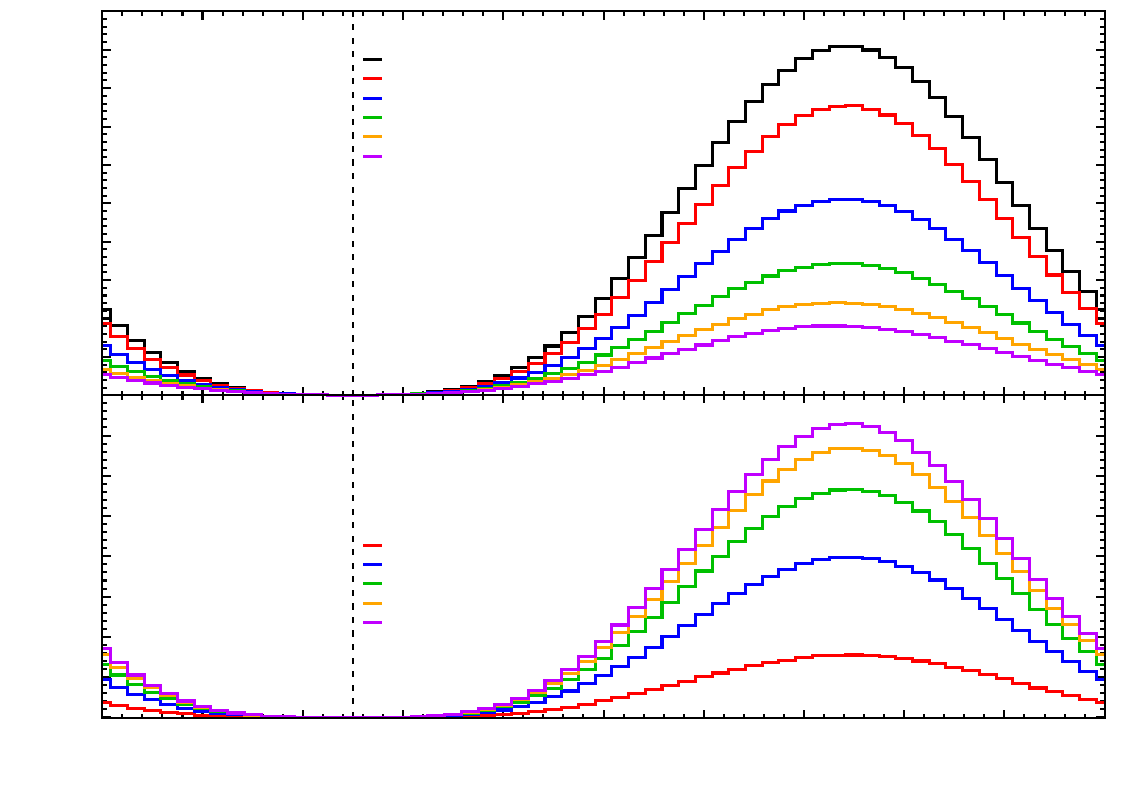
\includegraphics{pics/nuenorm_anti_chi2_dCP}}%
    \gplfronttext
  \end{picture}%
\endgroup
}
	\caption{$\chi^2$ profile for $\delta_\text{CP}$ for correlated (left) and anticorrelated (right) systematics. 
		The bottom panels show the difference of the different lines with the no systematic profile.}
	\label{fig:nuenorm_dCP}
\end{figure}

\begin{figure}
	\centering
	\resizebox{0.48\linewidth}{!}{% GNUPLOT: LaTeX picture with Postscript
\begingroup
  \makeatletter
  \providecommand\color[2][]{%
    \GenericError{(gnuplot) \space\space\space\@spaces}{%
      Package color not loaded in conjunction with
      terminal option `colourtext'%
    }{See the gnuplot documentation for explanation.%
    }{Either use 'blacktext' in gnuplot or load the package
      color.sty in LaTeX.}%
    \renewcommand\color[2][]{}%
  }%
  \providecommand\includegraphics[2][]{%
    \GenericError{(gnuplot) \space\space\space\@spaces}{%
      Package graphicx or graphics not loaded%
    }{See the gnuplot documentation for explanation.%
    }{The gnuplot epslatex terminal needs graphicx.sty or graphics.sty.}%
    \renewcommand\includegraphics[2][]{}%
  }%
  \providecommand\rotatebox[2]{#2}%
  \@ifundefined{ifGPcolor}{%
    \newif\ifGPcolor
    \GPcolortrue
  }{}%
  \@ifundefined{ifGPblacktext}{%
    \newif\ifGPblacktext
    \GPblacktexttrue
  }{}%
  % define a \g@addto@macro without @ in the name:
  \let\gplgaddtomacro\g@addto@macro
  % define empty templates for all commands taking text:
  \gdef\gplbacktext{}%
  \gdef\gplfronttext{}%
  \makeatother
  \ifGPblacktext
    % no textcolor at all
    \def\colorrgb#1{}%
    \def\colorgray#1{}%
  \else
    % gray or color?
    \ifGPcolor
      \def\colorrgb#1{\color[rgb]{#1}}%
      \def\colorgray#1{\color[gray]{#1}}%
      \expandafter\def\csname LTw\endcsname{\color{white}}%
      \expandafter\def\csname LTb\endcsname{\color{black}}%
      \expandafter\def\csname LTa\endcsname{\color{black}}%
      \expandafter\def\csname LT0\endcsname{\color[rgb]{1,0,0}}%
      \expandafter\def\csname LT1\endcsname{\color[rgb]{0,1,0}}%
      \expandafter\def\csname LT2\endcsname{\color[rgb]{0,0,1}}%
      \expandafter\def\csname LT3\endcsname{\color[rgb]{1,0,1}}%
      \expandafter\def\csname LT4\endcsname{\color[rgb]{0,1,1}}%
      \expandafter\def\csname LT5\endcsname{\color[rgb]{1,1,0}}%
      \expandafter\def\csname LT6\endcsname{\color[rgb]{0,0,0}}%
      \expandafter\def\csname LT7\endcsname{\color[rgb]{1,0.3,0}}%
      \expandafter\def\csname LT8\endcsname{\color[rgb]{0.5,0.5,0.5}}%
    \else
      % gray
      \def\colorrgb#1{\color{black}}%
      \def\colorgray#1{\color[gray]{#1}}%
      \expandafter\def\csname LTw\endcsname{\color{white}}%
      \expandafter\def\csname LTb\endcsname{\color{black}}%
      \expandafter\def\csname LTa\endcsname{\color{black}}%
      \expandafter\def\csname LT0\endcsname{\color{black}}%
      \expandafter\def\csname LT1\endcsname{\color{black}}%
      \expandafter\def\csname LT2\endcsname{\color{black}}%
      \expandafter\def\csname LT3\endcsname{\color{black}}%
      \expandafter\def\csname LT4\endcsname{\color{black}}%
      \expandafter\def\csname LT5\endcsname{\color{black}}%
      \expandafter\def\csname LT6\endcsname{\color{black}}%
      \expandafter\def\csname LT7\endcsname{\color{black}}%
      \expandafter\def\csname LT8\endcsname{\color{black}}%
    \fi
  \fi
    \setlength{\unitlength}{0.0500bp}%
    \ifx\gptboxheight\undefined%
      \newlength{\gptboxheight}%
      \newlength{\gptboxwidth}%
      \newsavebox{\gptboxtext}%
    \fi%
    \setlength{\fboxrule}{0.5pt}%
    \setlength{\fboxsep}{1pt}%
\begin{picture}(10800.00,7560.00)%
    \gplgaddtomacro\gplbacktext{%
      \csname LTb\endcsname%%
      \put(870,1024){\makebox(0,0)[r]{\strut{}0}}%
      \csname LTb\endcsname%%
      \put(870,1713){\makebox(0,0)[r]{\strut{}1}}%
      \csname LTb\endcsname%%
      \put(870,2402){\makebox(0,0)[r]{\strut{}2}}%
      \csname LTb\endcsname%%
      \put(870,3091){\makebox(0,0)[r]{\strut{}3}}%
      \csname LTb\endcsname%%
      \put(1614,494){\makebox(0,0){\strut{}2.47}}%
      \csname LTb\endcsname%%
      \put(2683,494){\makebox(0,0){\strut{}2.48}}%
      \csname LTb\endcsname%%
      \put(3752,494){\makebox(0,0){\strut{}2.49}}%
      \csname LTb\endcsname%%
      \put(4821,494){\makebox(0,0){\strut{}2.5}}%
      \csname LTb\endcsname%%
      \put(5890,494){\makebox(0,0){\strut{}2.51}}%
      \csname LTb\endcsname%%
      \put(6960,494){\makebox(0,0){\strut{}2.52}}%
      \csname LTb\endcsname%%
      \put(8029,494){\makebox(0,0){\strut{}2.53}}%
      \csname LTb\endcsname%%
      \put(9098,494){\makebox(0,0){\strut{}2.54}}%
      \csname LTb\endcsname%%
      \put(10167,494){\makebox(0,0){\strut{}2.55}}%
    }%
    \gplgaddtomacro\gplfronttext{%
      \csname LTb\endcsname%%
      \put(582,2230){\rotatebox{-270}{\makebox(0,0){\strut{}$\Delta \chi^2 - \Delta \chi^2_0$}}}%
      \csname LTb\endcsname%%
      \put(5783,215){\makebox(0,0){\strut{}$\Delta m_{32}^2 / 10^{-3}$}}%
      \csname LTb\endcsname%%
      \put(6637,2998){\makebox(0,0){\strut{}Difference}}%
      \csname LTb\endcsname%%
      \put(6164,2812){\makebox(0,0)[l]{\strut{}$1\%$}}%
      \csname LTb\endcsname%%
      \put(6164,2626){\makebox(0,0)[l]{\strut{}$2\%$}}%
      \csname LTb\endcsname%%
      \put(6164,2440){\makebox(0,0)[l]{\strut{}$3\%$}}%
      \csname LTb\endcsname%%
      \put(6164,2254){\makebox(0,0)[l]{\strut{}$4\%$}}%
      \csname LTb\endcsname%%
      \put(6164,2068){\makebox(0,0)[l]{\strut{}$5\%$}}%
    }%
    \gplgaddtomacro\gplbacktext{%
      \csname LTb\endcsname%%
      \put(870,3780){\makebox(0,0)[r]{\strut{}0}}%
      \csname LTb\endcsname%%
      \put(870,4532){\makebox(0,0)[r]{\strut{}10}}%
      \csname LTb\endcsname%%
      \put(870,5284){\makebox(0,0)[r]{\strut{}20}}%
      \csname LTb\endcsname%%
      \put(870,6037){\makebox(0,0)[r]{\strut{}30}}%
      \csname LTb\endcsname%%
      \put(870,6789){\makebox(0,0)[r]{\strut{}40}}%
      \csname LTb\endcsname%%
      \put(1614,3594){\makebox(0,0){\strut{}}}%
      \csname LTb\endcsname%%
      \put(2683,3594){\makebox(0,0){\strut{}}}%
      \csname LTb\endcsname%%
      \put(3752,3594){\makebox(0,0){\strut{}}}%
      \csname LTb\endcsname%%
      \put(4821,3594){\makebox(0,0){\strut{}}}%
      \csname LTb\endcsname%%
      \put(5890,3594){\makebox(0,0){\strut{}}}%
      \csname LTb\endcsname%%
      \put(6960,3594){\makebox(0,0){\strut{}}}%
      \csname LTb\endcsname%%
      \put(8029,3594){\makebox(0,0){\strut{}}}%
      \csname LTb\endcsname%%
      \put(9098,3594){\makebox(0,0){\strut{}}}%
      \csname LTb\endcsname%%
      \put(10167,3594){\makebox(0,0){\strut{}}}%
    }%
    \gplgaddtomacro\gplfronttext{%
      \csname LTb\endcsname%%
      \put(480,5623){\rotatebox{-270}{\makebox(0,0){\strut{}$\Delta \chi^2$}}}%
      \csname LTb\endcsname%%
      \put(5783,3538){\makebox(0,0){\strut{}}}%
      \csname LTb\endcsname%%
      \put(6637,7004){\makebox(0,0){\strut{}}}%
      \csname LTb\endcsname%%
      \put(6164,7004){\makebox(0,0)[l]{\strut{}No syst}}%
      \csname LTb\endcsname%%
      \put(6164,6818){\makebox(0,0)[l]{\strut{}$1\%$}}%
      \csname LTb\endcsname%%
      \put(6164,6632){\makebox(0,0)[l]{\strut{}$2\%$}}%
      \csname LTb\endcsname%%
      \put(6164,6446){\makebox(0,0)[l]{\strut{}$3\%$}}%
      \csname LTb\endcsname%%
      \put(6164,6260){\makebox(0,0)[l]{\strut{}$4\%$}}%
      \csname LTb\endcsname%%
      \put(6164,6074){\makebox(0,0)[l]{\strut{}$5\%$}}%
    }%
    \gplbacktext
    \put(0,0){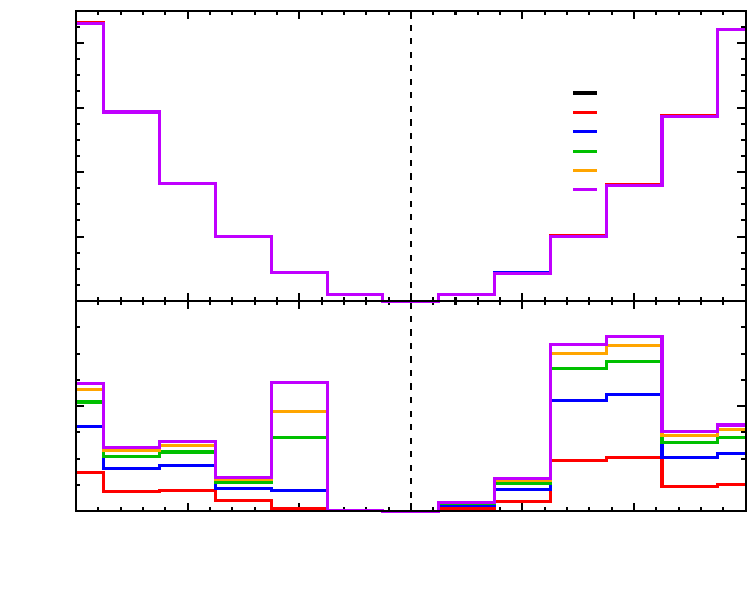
\includegraphics{pics/nuenorm_corr_chi2_M23}}%
    \gplfronttext
  \end{picture}%
\endgroup
}
	\resizebox{0.48\linewidth}{!}{% GNUPLOT: LaTeX picture with Postscript
\begingroup
  \makeatletter
  \providecommand\color[2][]{%
    \GenericError{(gnuplot) \space\space\space\@spaces}{%
      Package color not loaded in conjunction with
      terminal option `colourtext'%
    }{See the gnuplot documentation for explanation.%
    }{Either use 'blacktext' in gnuplot or load the package
      color.sty in LaTeX.}%
    \renewcommand\color[2][]{}%
  }%
  \providecommand\includegraphics[2][]{%
    \GenericError{(gnuplot) \space\space\space\@spaces}{%
      Package graphicx or graphics not loaded%
    }{See the gnuplot documentation for explanation.%
    }{The gnuplot epslatex terminal needs graphicx.sty or graphics.sty.}%
    \renewcommand\includegraphics[2][]{}%
  }%
  \providecommand\rotatebox[2]{#2}%
  \@ifundefined{ifGPcolor}{%
    \newif\ifGPcolor
    \GPcolortrue
  }{}%
  \@ifundefined{ifGPblacktext}{%
    \newif\ifGPblacktext
    \GPblacktexttrue
  }{}%
  % define a \g@addto@macro without @ in the name:
  \let\gplgaddtomacro\g@addto@macro
  % define empty templates for all commands taking text:
  \gdef\gplbacktext{}%
  \gdef\gplfronttext{}%
  \makeatother
  \ifGPblacktext
    % no textcolor at all
    \def\colorrgb#1{}%
    \def\colorgray#1{}%
  \else
    % gray or color?
    \ifGPcolor
      \def\colorrgb#1{\color[rgb]{#1}}%
      \def\colorgray#1{\color[gray]{#1}}%
      \expandafter\def\csname LTw\endcsname{\color{white}}%
      \expandafter\def\csname LTb\endcsname{\color{black}}%
      \expandafter\def\csname LTa\endcsname{\color{black}}%
      \expandafter\def\csname LT0\endcsname{\color[rgb]{1,0,0}}%
      \expandafter\def\csname LT1\endcsname{\color[rgb]{0,1,0}}%
      \expandafter\def\csname LT2\endcsname{\color[rgb]{0,0,1}}%
      \expandafter\def\csname LT3\endcsname{\color[rgb]{1,0,1}}%
      \expandafter\def\csname LT4\endcsname{\color[rgb]{0,1,1}}%
      \expandafter\def\csname LT5\endcsname{\color[rgb]{1,1,0}}%
      \expandafter\def\csname LT6\endcsname{\color[rgb]{0,0,0}}%
      \expandafter\def\csname LT7\endcsname{\color[rgb]{1,0.3,0}}%
      \expandafter\def\csname LT8\endcsname{\color[rgb]{0.5,0.5,0.5}}%
    \else
      % gray
      \def\colorrgb#1{\color{black}}%
      \def\colorgray#1{\color[gray]{#1}}%
      \expandafter\def\csname LTw\endcsname{\color{white}}%
      \expandafter\def\csname LTb\endcsname{\color{black}}%
      \expandafter\def\csname LTa\endcsname{\color{black}}%
      \expandafter\def\csname LT0\endcsname{\color{black}}%
      \expandafter\def\csname LT1\endcsname{\color{black}}%
      \expandafter\def\csname LT2\endcsname{\color{black}}%
      \expandafter\def\csname LT3\endcsname{\color{black}}%
      \expandafter\def\csname LT4\endcsname{\color{black}}%
      \expandafter\def\csname LT5\endcsname{\color{black}}%
      \expandafter\def\csname LT6\endcsname{\color{black}}%
      \expandafter\def\csname LT7\endcsname{\color{black}}%
      \expandafter\def\csname LT8\endcsname{\color{black}}%
    \fi
  \fi
    \setlength{\unitlength}{0.0500bp}%
    \ifx\gptboxheight\undefined%
      \newlength{\gptboxheight}%
      \newlength{\gptboxwidth}%
      \newsavebox{\gptboxtext}%
    \fi%
    \setlength{\fboxrule}{0.5pt}%
    \setlength{\fboxsep}{1pt}%
\begin{picture}(7200.00,5760.00)%
    \gplgaddtomacro\gplbacktext{%
      \csname LTb\endcsname%%
      \put(618,864){\makebox(0,0)[r]{\strut{}0}}%
      \csname LTb\endcsname%%
      \put(618,1368){\makebox(0,0)[r]{\strut{}1}}%
      \csname LTb\endcsname%%
      \put(618,1872){\makebox(0,0)[r]{\strut{}2}}%
      \csname LTb\endcsname%%
      \put(618,2376){\makebox(0,0)[r]{\strut{}3}}%
      \csname LTb\endcsname%%
      \put(720,678){\makebox(0,0){\strut{}2.464}}%
      \csname LTb\endcsname%%
      \put(1791,678){\makebox(0,0){\strut{}2.479}}%
      \csname LTb\endcsname%%
      \put(2863,678){\makebox(0,0){\strut{}2.494}}%
      \csname LTb\endcsname%%
      \put(3934,678){\makebox(0,0){\strut{}2.509}}%
      \csname LTb\endcsname%%
      \put(5005,678){\makebox(0,0){\strut{}2.524}}%
      \csname LTb\endcsname%%
      \put(6077,678){\makebox(0,0){\strut{}2.539}}%
      \csname LTb\endcsname%%
      \put(7148,678){\makebox(0,0){\strut{}2.554}}%
    }%
    \gplgaddtomacro\gplfronttext{%
      \csname LTb\endcsname%%
      \put(330,1872){\rotatebox{-270}{\makebox(0,0){\strut{}$\Delta \chi^2_\text{No syst} - \Delta \chi^2$}}}%
      \csname LTb\endcsname%%
      \put(3934,399){\makebox(0,0){\strut{}$\Delta m_{32}^2 / 10^{-3}$}}%
    }%
    \gplgaddtomacro\gplbacktext{%
      \csname LTb\endcsname%%
      \put(618,2880){\makebox(0,0)[r]{\strut{}0}}%
      \csname LTb\endcsname%%
      \put(618,3499){\makebox(0,0)[r]{\strut{}10}}%
      \csname LTb\endcsname%%
      \put(618,4118){\makebox(0,0)[r]{\strut{}20}}%
      \csname LTb\endcsname%%
      \put(618,4737){\makebox(0,0)[r]{\strut{}30}}%
      \csname LTb\endcsname%%
      \put(618,5356){\makebox(0,0)[r]{\strut{}40}}%
      \csname LTb\endcsname%%
      \put(720,2694){\makebox(0,0){\strut{}}}%
      \csname LTb\endcsname%%
      \put(1791,2694){\makebox(0,0){\strut{}}}%
      \csname LTb\endcsname%%
      \put(2863,2694){\makebox(0,0){\strut{}}}%
      \csname LTb\endcsname%%
      \put(3934,2694){\makebox(0,0){\strut{}}}%
      \csname LTb\endcsname%%
      \put(5005,2694){\makebox(0,0){\strut{}}}%
      \csname LTb\endcsname%%
      \put(6077,2694){\makebox(0,0){\strut{}}}%
      \csname LTb\endcsname%%
      \put(7148,2694){\makebox(0,0){\strut{}}}%
    }%
    \gplgaddtomacro\gplfronttext{%
      \csname LTb\endcsname%%
      \put(228,4273){\rotatebox{-270}{\makebox(0,0){\strut{}$\Delta \chi^2$}}}%
      \csname LTb\endcsname%%
      \put(3934,2638){\makebox(0,0){\strut{}}}%
      \csname LTb\endcsname%%
      \put(4941,4877){\makebox(0,0){\strut{}}}%
      \csname LTb\endcsname%%
      \put(5389,4877){\makebox(0,0)[r]{\strut{}No syst}}%
      \csname LTb\endcsname%%
      \put(5389,4691){\makebox(0,0)[r]{\strut{}1\,\%}}%
      \csname LTb\endcsname%%
      \put(5389,4505){\makebox(0,0)[r]{\strut{}2\,\%}}%
      \csname LTb\endcsname%%
      \put(5389,4319){\makebox(0,0)[r]{\strut{}3\,\%}}%
      \csname LTb\endcsname%%
      \put(5389,4133){\makebox(0,0)[r]{\strut{}4\,\%}}%
      \csname LTb\endcsname%%
      \put(5389,3947){\makebox(0,0)[r]{\strut{}5\,\%}}%
    }%
    \gplbacktext
    \put(0,0){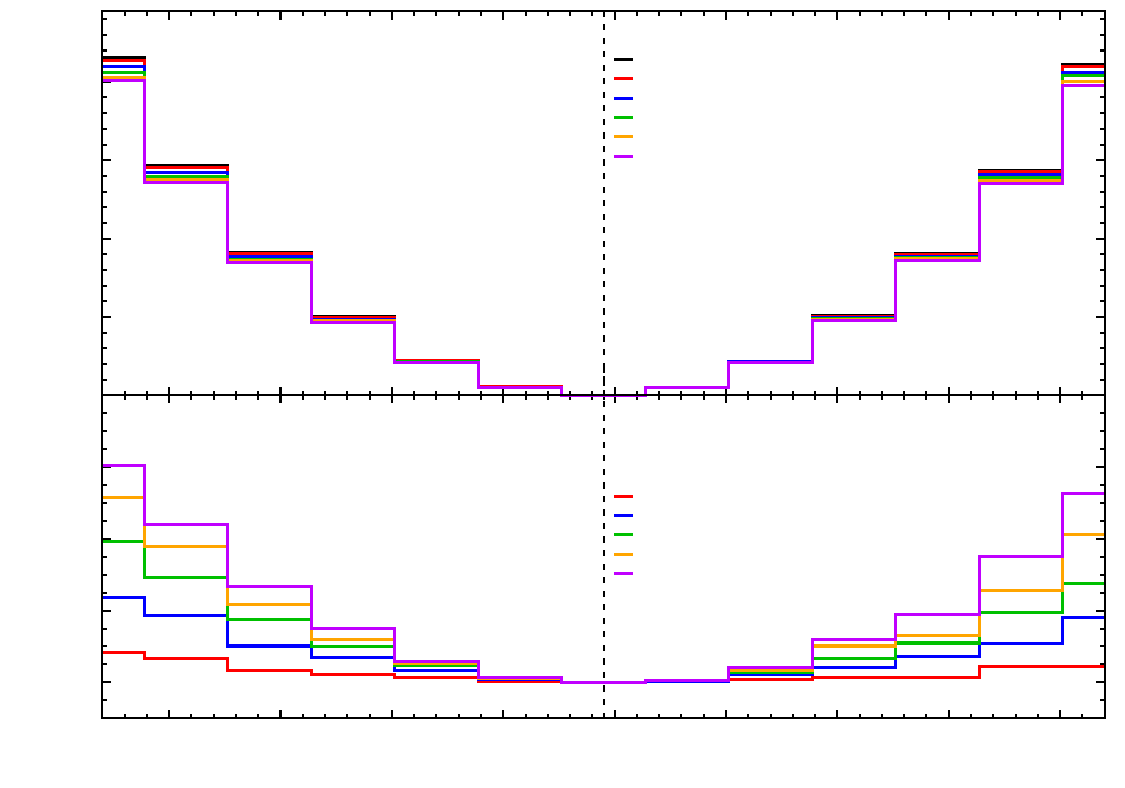
\includegraphics{pics/nuenorm_anti_chi2_M23}}%
    \gplfronttext
  \end{picture}%
\endgroup
}
	\caption{$\chi^2$ profile for $\Delta m_{32}^2$ for correlated (left) and anticorrelated (right) systematics. 
		The bottom panels show the difference of the different lines with the no systematic profile.}
	\label{fig:nuenorm_M23}
\end{figure}

\begin{figure}
	\centering
	\resizebox{0.48\linewidth}{!}{% GNUPLOT: LaTeX picture with Postscript
\begingroup
  \makeatletter
  \providecommand\color[2][]{%
    \GenericError{(gnuplot) \space\space\space\@spaces}{%
      Package color not loaded in conjunction with
      terminal option `colourtext'%
    }{See the gnuplot documentation for explanation.%
    }{Either use 'blacktext' in gnuplot or load the package
      color.sty in LaTeX.}%
    \renewcommand\color[2][]{}%
  }%
  \providecommand\includegraphics[2][]{%
    \GenericError{(gnuplot) \space\space\space\@spaces}{%
      Package graphicx or graphics not loaded%
    }{See the gnuplot documentation for explanation.%
    }{The gnuplot epslatex terminal needs graphicx.sty or graphics.sty.}%
    \renewcommand\includegraphics[2][]{}%
  }%
  \providecommand\rotatebox[2]{#2}%
  \@ifundefined{ifGPcolor}{%
    \newif\ifGPcolor
    \GPcolortrue
  }{}%
  \@ifundefined{ifGPblacktext}{%
    \newif\ifGPblacktext
    \GPblacktexttrue
  }{}%
  % define a \g@addto@macro without @ in the name:
  \let\gplgaddtomacro\g@addto@macro
  % define empty templates for all commands taking text:
  \gdef\gplbacktext{}%
  \gdef\gplfronttext{}%
  \makeatother
  \ifGPblacktext
    % no textcolor at all
    \def\colorrgb#1{}%
    \def\colorgray#1{}%
  \else
    % gray or color?
    \ifGPcolor
      \def\colorrgb#1{\color[rgb]{#1}}%
      \def\colorgray#1{\color[gray]{#1}}%
      \expandafter\def\csname LTw\endcsname{\color{white}}%
      \expandafter\def\csname LTb\endcsname{\color{black}}%
      \expandafter\def\csname LTa\endcsname{\color{black}}%
      \expandafter\def\csname LT0\endcsname{\color[rgb]{1,0,0}}%
      \expandafter\def\csname LT1\endcsname{\color[rgb]{0,1,0}}%
      \expandafter\def\csname LT2\endcsname{\color[rgb]{0,0,1}}%
      \expandafter\def\csname LT3\endcsname{\color[rgb]{1,0,1}}%
      \expandafter\def\csname LT4\endcsname{\color[rgb]{0,1,1}}%
      \expandafter\def\csname LT5\endcsname{\color[rgb]{1,1,0}}%
      \expandafter\def\csname LT6\endcsname{\color[rgb]{0,0,0}}%
      \expandafter\def\csname LT7\endcsname{\color[rgb]{1,0.3,0}}%
      \expandafter\def\csname LT8\endcsname{\color[rgb]{0.5,0.5,0.5}}%
    \else
      % gray
      \def\colorrgb#1{\color{black}}%
      \def\colorgray#1{\color[gray]{#1}}%
      \expandafter\def\csname LTw\endcsname{\color{white}}%
      \expandafter\def\csname LTb\endcsname{\color{black}}%
      \expandafter\def\csname LTa\endcsname{\color{black}}%
      \expandafter\def\csname LT0\endcsname{\color{black}}%
      \expandafter\def\csname LT1\endcsname{\color{black}}%
      \expandafter\def\csname LT2\endcsname{\color{black}}%
      \expandafter\def\csname LT3\endcsname{\color{black}}%
      \expandafter\def\csname LT4\endcsname{\color{black}}%
      \expandafter\def\csname LT5\endcsname{\color{black}}%
      \expandafter\def\csname LT6\endcsname{\color{black}}%
      \expandafter\def\csname LT7\endcsname{\color{black}}%
      \expandafter\def\csname LT8\endcsname{\color{black}}%
    \fi
  \fi
    \setlength{\unitlength}{0.0500bp}%
    \ifx\gptboxheight\undefined%
      \newlength{\gptboxheight}%
      \newlength{\gptboxwidth}%
      \newsavebox{\gptboxtext}%
    \fi%
    \setlength{\fboxrule}{0.5pt}%
    \setlength{\fboxsep}{1pt}%
\begin{picture}(7200.00,5760.00)%
    \gplgaddtomacro\gplbacktext{%
      \csname LTb\endcsname%%
      \put(618,864){\makebox(0,0)[r]{\strut{}0}}%
      \csname LTb\endcsname%%
      \put(618,1200){\makebox(0,0)[r]{\strut{}10}}%
      \csname LTb\endcsname%%
      \put(618,1536){\makebox(0,0)[r]{\strut{}20}}%
      \csname LTb\endcsname%%
      \put(618,1872){\makebox(0,0)[r]{\strut{}30}}%
      \csname LTb\endcsname%%
      \put(618,2208){\makebox(0,0)[r]{\strut{}40}}%
      \csname LTb\endcsname%%
      \put(618,2544){\makebox(0,0)[r]{\strut{}50}}%
      \csname LTb\endcsname%%
      \put(720,678){\makebox(0,0){\strut{}0.07}}%
      \csname LTb\endcsname%%
      \put(1791,678){\makebox(0,0){\strut{}0.075}}%
      \csname LTb\endcsname%%
      \put(2863,678){\makebox(0,0){\strut{}0.08}}%
      \csname LTb\endcsname%%
      \put(3934,678){\makebox(0,0){\strut{}0.085}}%
      \csname LTb\endcsname%%
      \put(5005,678){\makebox(0,0){\strut{}0.09}}%
      \csname LTb\endcsname%%
      \put(6077,678){\makebox(0,0){\strut{}0.095}}%
      \csname LTb\endcsname%%
      \put(7148,678){\makebox(0,0){\strut{}0.1}}%
    }%
    \gplgaddtomacro\gplfronttext{%
      \csname LTb\endcsname%%
      \put(228,1872){\rotatebox{-270}{\makebox(0,0){\strut{}$\Delta \chi^2_\text{No syst} - \Delta \chi^2$}}}%
      \csname LTb\endcsname%%
      \put(3934,399){\makebox(0,0){\strut{}$\sin^2 2 \theta_{13}$}}%
    }%
    \gplgaddtomacro\gplbacktext{%
      \csname LTb\endcsname%%
      \put(618,2880){\makebox(0,0)[r]{\strut{}0}}%
      \csname LTb\endcsname%%
      \put(618,3577){\makebox(0,0)[r]{\strut{}20}}%
      \csname LTb\endcsname%%
      \put(618,4273){\makebox(0,0)[r]{\strut{}40}}%
      \csname LTb\endcsname%%
      \put(618,4970){\makebox(0,0)[r]{\strut{}60}}%
      \csname LTb\endcsname%%
      \put(618,5666){\makebox(0,0)[r]{\strut{}80}}%
      \csname LTb\endcsname%%
      \put(720,2694){\makebox(0,0){\strut{}}}%
      \csname LTb\endcsname%%
      \put(1791,2694){\makebox(0,0){\strut{}}}%
      \csname LTb\endcsname%%
      \put(2863,2694){\makebox(0,0){\strut{}}}%
      \csname LTb\endcsname%%
      \put(3934,2694){\makebox(0,0){\strut{}}}%
      \csname LTb\endcsname%%
      \put(5005,2694){\makebox(0,0){\strut{}}}%
      \csname LTb\endcsname%%
      \put(6077,2694){\makebox(0,0){\strut{}}}%
      \csname LTb\endcsname%%
      \put(7148,2694){\makebox(0,0){\strut{}}}%
    }%
    \gplgaddtomacro\gplfronttext{%
      \csname LTb\endcsname%%
      \put(228,4273){\rotatebox{-270}{\makebox(0,0){\strut{}$\Delta \chi^2$}}}%
      \csname LTb\endcsname%%
      \put(3934,2638){\makebox(0,0){\strut{}}}%
      \csname LTb\endcsname%%
      \put(4954,4877){\makebox(0,0){\strut{}}}%
      \csname LTb\endcsname%%
      \put(5402,4877){\makebox(0,0)[r]{\strut{}No syst}}%
      \csname LTb\endcsname%%
      \put(5402,4691){\makebox(0,0)[r]{\strut{}1\,\%}}%
      \csname LTb\endcsname%%
      \put(5402,4505){\makebox(0,0)[r]{\strut{}2\,\%}}%
      \csname LTb\endcsname%%
      \put(5402,4319){\makebox(0,0)[r]{\strut{}3\,\%}}%
      \csname LTb\endcsname%%
      \put(5402,4133){\makebox(0,0)[r]{\strut{}4\,\%}}%
      \csname LTb\endcsname%%
      \put(5402,3947){\makebox(0,0)[r]{\strut{}5\,\%}}%
    }%
    \gplbacktext
    \put(0,0){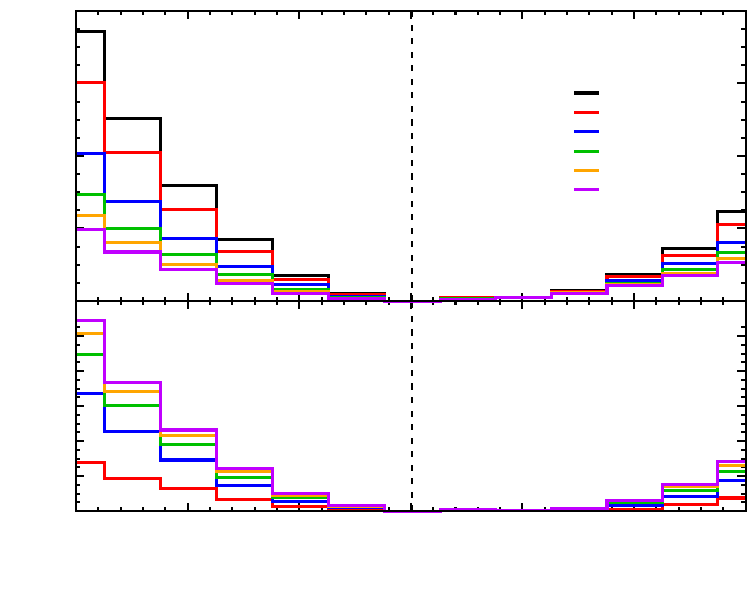
\includegraphics{pics/nuenorm_corr_chi2_S13}}%
    \gplfronttext
  \end{picture}%
\endgroup
}
	\resizebox{0.48\linewidth}{!}{% GNUPLOT: LaTeX picture with Postscript
\begingroup
  \makeatletter
  \providecommand\color[2][]{%
    \GenericError{(gnuplot) \space\space\space\@spaces}{%
      Package color not loaded in conjunction with
      terminal option `colourtext'%
    }{See the gnuplot documentation for explanation.%
    }{Either use 'blacktext' in gnuplot or load the package
      color.sty in LaTeX.}%
    \renewcommand\color[2][]{}%
  }%
  \providecommand\includegraphics[2][]{%
    \GenericError{(gnuplot) \space\space\space\@spaces}{%
      Package graphicx or graphics not loaded%
    }{See the gnuplot documentation for explanation.%
    }{The gnuplot epslatex terminal needs graphicx.sty or graphics.sty.}%
    \renewcommand\includegraphics[2][]{}%
  }%
  \providecommand\rotatebox[2]{#2}%
  \@ifundefined{ifGPcolor}{%
    \newif\ifGPcolor
    \GPcolortrue
  }{}%
  \@ifundefined{ifGPblacktext}{%
    \newif\ifGPblacktext
    \GPblacktexttrue
  }{}%
  % define a \g@addto@macro without @ in the name:
  \let\gplgaddtomacro\g@addto@macro
  % define empty templates for all commands taking text:
  \gdef\gplbacktext{}%
  \gdef\gplfronttext{}%
  \makeatother
  \ifGPblacktext
    % no textcolor at all
    \def\colorrgb#1{}%
    \def\colorgray#1{}%
  \else
    % gray or color?
    \ifGPcolor
      \def\colorrgb#1{\color[rgb]{#1}}%
      \def\colorgray#1{\color[gray]{#1}}%
      \expandafter\def\csname LTw\endcsname{\color{white}}%
      \expandafter\def\csname LTb\endcsname{\color{black}}%
      \expandafter\def\csname LTa\endcsname{\color{black}}%
      \expandafter\def\csname LT0\endcsname{\color[rgb]{1,0,0}}%
      \expandafter\def\csname LT1\endcsname{\color[rgb]{0,1,0}}%
      \expandafter\def\csname LT2\endcsname{\color[rgb]{0,0,1}}%
      \expandafter\def\csname LT3\endcsname{\color[rgb]{1,0,1}}%
      \expandafter\def\csname LT4\endcsname{\color[rgb]{0,1,1}}%
      \expandafter\def\csname LT5\endcsname{\color[rgb]{1,1,0}}%
      \expandafter\def\csname LT6\endcsname{\color[rgb]{0,0,0}}%
      \expandafter\def\csname LT7\endcsname{\color[rgb]{1,0.3,0}}%
      \expandafter\def\csname LT8\endcsname{\color[rgb]{0.5,0.5,0.5}}%
    \else
      % gray
      \def\colorrgb#1{\color{black}}%
      \def\colorgray#1{\color[gray]{#1}}%
      \expandafter\def\csname LTw\endcsname{\color{white}}%
      \expandafter\def\csname LTb\endcsname{\color{black}}%
      \expandafter\def\csname LTa\endcsname{\color{black}}%
      \expandafter\def\csname LT0\endcsname{\color{black}}%
      \expandafter\def\csname LT1\endcsname{\color{black}}%
      \expandafter\def\csname LT2\endcsname{\color{black}}%
      \expandafter\def\csname LT3\endcsname{\color{black}}%
      \expandafter\def\csname LT4\endcsname{\color{black}}%
      \expandafter\def\csname LT5\endcsname{\color{black}}%
      \expandafter\def\csname LT6\endcsname{\color{black}}%
      \expandafter\def\csname LT7\endcsname{\color{black}}%
      \expandafter\def\csname LT8\endcsname{\color{black}}%
    \fi
  \fi
    \setlength{\unitlength}{0.0500bp}%
    \ifx\gptboxheight\undefined%
      \newlength{\gptboxheight}%
      \newlength{\gptboxwidth}%
      \newsavebox{\gptboxtext}%
    \fi%
    \setlength{\fboxrule}{0.5pt}%
    \setlength{\fboxsep}{1pt}%
\begin{picture}(7200.00,5760.00)%
    \gplgaddtomacro\gplbacktext{%
      \csname LTb\endcsname%%
      \put(618,864){\makebox(0,0)[r]{\strut{}0}}%
      \csname LTb\endcsname%%
      \put(618,1872){\makebox(0,0)[r]{\strut{}10}}%
      \csname LTb\endcsname%%
      \put(720,678){\makebox(0,0){\strut{}0.07}}%
      \csname LTb\endcsname%%
      \put(1791,678){\makebox(0,0){\strut{}0.075}}%
      \csname LTb\endcsname%%
      \put(2863,678){\makebox(0,0){\strut{}0.08}}%
      \csname LTb\endcsname%%
      \put(3934,678){\makebox(0,0){\strut{}0.085}}%
      \csname LTb\endcsname%%
      \put(5005,678){\makebox(0,0){\strut{}0.09}}%
      \csname LTb\endcsname%%
      \put(6077,678){\makebox(0,0){\strut{}0.095}}%
      \csname LTb\endcsname%%
      \put(7148,678){\makebox(0,0){\strut{}0.1}}%
    }%
    \gplgaddtomacro\gplfronttext{%
      \csname LTb\endcsname%%
      \put(228,1872){\rotatebox{-270}{\makebox(0,0){\strut{}$\Delta \chi^2_\text{No syst} - \Delta \chi^2$}}}%
      \csname LTb\endcsname%%
      \put(3934,399){\makebox(0,0){\strut{}$\sin^2 2 \theta_{13}$}}%
    }%
    \gplgaddtomacro\gplbacktext{%
      \csname LTb\endcsname%%
      \put(618,2880){\makebox(0,0)[r]{\strut{}0}}%
      \csname LTb\endcsname%%
      \put(618,3577){\makebox(0,0)[r]{\strut{}20}}%
      \csname LTb\endcsname%%
      \put(618,4273){\makebox(0,0)[r]{\strut{}40}}%
      \csname LTb\endcsname%%
      \put(618,4970){\makebox(0,0)[r]{\strut{}60}}%
      \csname LTb\endcsname%%
      \put(618,5666){\makebox(0,0)[r]{\strut{}80}}%
      \csname LTb\endcsname%%
      \put(720,2694){\makebox(0,0){\strut{}}}%
      \csname LTb\endcsname%%
      \put(1791,2694){\makebox(0,0){\strut{}}}%
      \csname LTb\endcsname%%
      \put(2863,2694){\makebox(0,0){\strut{}}}%
      \csname LTb\endcsname%%
      \put(3934,2694){\makebox(0,0){\strut{}}}%
      \csname LTb\endcsname%%
      \put(5005,2694){\makebox(0,0){\strut{}}}%
      \csname LTb\endcsname%%
      \put(6077,2694){\makebox(0,0){\strut{}}}%
      \csname LTb\endcsname%%
      \put(7148,2694){\makebox(0,0){\strut{}}}%
    }%
    \gplgaddtomacro\gplfronttext{%
      \csname LTb\endcsname%%
      \put(228,4273){\rotatebox{-270}{\makebox(0,0){\strut{}$\Delta \chi^2$}}}%
      \csname LTb\endcsname%%
      \put(3934,2638){\makebox(0,0){\strut{}}}%
      \csname LTb\endcsname%%
      \put(4954,4877){\makebox(0,0){\strut{}}}%
      \csname LTb\endcsname%%
      \put(5402,4877){\makebox(0,0)[r]{\strut{}No syst}}%
      \csname LTb\endcsname%%
      \put(5402,4691){\makebox(0,0)[r]{\strut{}1\,\%}}%
      \csname LTb\endcsname%%
      \put(5402,4505){\makebox(0,0)[r]{\strut{}2\,\%}}%
      \csname LTb\endcsname%%
      \put(5402,4319){\makebox(0,0)[r]{\strut{}3\,\%}}%
      \csname LTb\endcsname%%
      \put(5402,4133){\makebox(0,0)[r]{\strut{}4\,\%}}%
      \csname LTb\endcsname%%
      \put(5402,3947){\makebox(0,0)[r]{\strut{}5\,\%}}%
    }%
    \gplbacktext
    \put(0,0){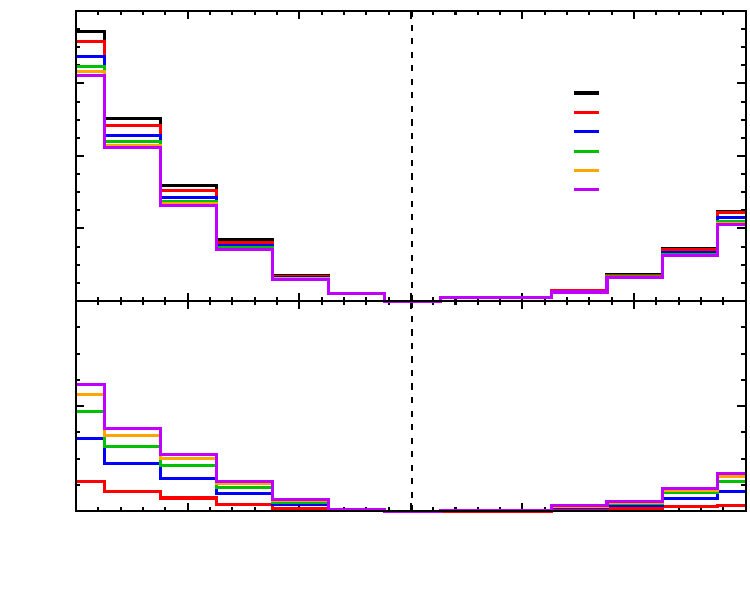
\includegraphics{pics/nuenorm_anti_chi2_S13}}%
    \gplfronttext
  \end{picture}%
\endgroup
}
	\caption{$\chi^2$ profile for $\sin^2 2\theta_{13}$ for correlated (left) and anticorrelated (right) systematics. 
		The bottom panels show the difference of the different lines with the no systematic profile.}
	\label{fig:nuenorm_S13}
\end{figure}

\begin{figure}
	\centering
	\resizebox{0.48\linewidth}{!}{% GNUPLOT: LaTeX picture with Postscript
\begingroup
  \makeatletter
  \providecommand\color[2][]{%
    \GenericError{(gnuplot) \space\space\space\@spaces}{%
      Package color not loaded in conjunction with
      terminal option `colourtext'%
    }{See the gnuplot documentation for explanation.%
    }{Either use 'blacktext' in gnuplot or load the package
      color.sty in LaTeX.}%
    \renewcommand\color[2][]{}%
  }%
  \providecommand\includegraphics[2][]{%
    \GenericError{(gnuplot) \space\space\space\@spaces}{%
      Package graphicx or graphics not loaded%
    }{See the gnuplot documentation for explanation.%
    }{The gnuplot epslatex terminal needs graphicx.sty or graphics.sty.}%
    \renewcommand\includegraphics[2][]{}%
  }%
  \providecommand\rotatebox[2]{#2}%
  \@ifundefined{ifGPcolor}{%
    \newif\ifGPcolor
    \GPcolortrue
  }{}%
  \@ifundefined{ifGPblacktext}{%
    \newif\ifGPblacktext
    \GPblacktexttrue
  }{}%
  % define a \g@addto@macro without @ in the name:
  \let\gplgaddtomacro\g@addto@macro
  % define empty templates for all commands taking text:
  \gdef\gplbacktext{}%
  \gdef\gplfronttext{}%
  \makeatother
  \ifGPblacktext
    % no textcolor at all
    \def\colorrgb#1{}%
    \def\colorgray#1{}%
  \else
    % gray or color?
    \ifGPcolor
      \def\colorrgb#1{\color[rgb]{#1}}%
      \def\colorgray#1{\color[gray]{#1}}%
      \expandafter\def\csname LTw\endcsname{\color{white}}%
      \expandafter\def\csname LTb\endcsname{\color{black}}%
      \expandafter\def\csname LTa\endcsname{\color{black}}%
      \expandafter\def\csname LT0\endcsname{\color[rgb]{1,0,0}}%
      \expandafter\def\csname LT1\endcsname{\color[rgb]{0,1,0}}%
      \expandafter\def\csname LT2\endcsname{\color[rgb]{0,0,1}}%
      \expandafter\def\csname LT3\endcsname{\color[rgb]{1,0,1}}%
      \expandafter\def\csname LT4\endcsname{\color[rgb]{0,1,1}}%
      \expandafter\def\csname LT5\endcsname{\color[rgb]{1,1,0}}%
      \expandafter\def\csname LT6\endcsname{\color[rgb]{0,0,0}}%
      \expandafter\def\csname LT7\endcsname{\color[rgb]{1,0.3,0}}%
      \expandafter\def\csname LT8\endcsname{\color[rgb]{0.5,0.5,0.5}}%
    \else
      % gray
      \def\colorrgb#1{\color{black}}%
      \def\colorgray#1{\color[gray]{#1}}%
      \expandafter\def\csname LTw\endcsname{\color{white}}%
      \expandafter\def\csname LTb\endcsname{\color{black}}%
      \expandafter\def\csname LTa\endcsname{\color{black}}%
      \expandafter\def\csname LT0\endcsname{\color{black}}%
      \expandafter\def\csname LT1\endcsname{\color{black}}%
      \expandafter\def\csname LT2\endcsname{\color{black}}%
      \expandafter\def\csname LT3\endcsname{\color{black}}%
      \expandafter\def\csname LT4\endcsname{\color{black}}%
      \expandafter\def\csname LT5\endcsname{\color{black}}%
      \expandafter\def\csname LT6\endcsname{\color{black}}%
      \expandafter\def\csname LT7\endcsname{\color{black}}%
      \expandafter\def\csname LT8\endcsname{\color{black}}%
    \fi
  \fi
    \setlength{\unitlength}{0.0500bp}%
    \ifx\gptboxheight\undefined%
      \newlength{\gptboxheight}%
      \newlength{\gptboxwidth}%
      \newsavebox{\gptboxtext}%
    \fi%
    \setlength{\fboxrule}{0.5pt}%
    \setlength{\fboxsep}{1pt}%
\begin{picture}(10800.00,7560.00)%
    \gplgaddtomacro\gplbacktext{%
      \csname LTb\endcsname%%
      \put(870,874){\makebox(0,0)[r]{\strut{}0}}%
      \csname LTb\endcsname%%
      \put(870,1358){\makebox(0,0)[r]{\strut{}5}}%
      \csname LTb\endcsname%%
      \put(870,1843){\makebox(0,0)[r]{\strut{}10}}%
      \csname LTb\endcsname%%
      \put(870,2327){\makebox(0,0)[r]{\strut{}15}}%
      \csname LTb\endcsname%%
      \put(870,2811){\makebox(0,0)[r]{\strut{}20}}%
      \csname LTb\endcsname%%
      \put(870,3296){\makebox(0,0)[r]{\strut{}25}}%
      \csname LTb\endcsname%%
      \put(1853,494){\makebox(0,0){\strut{}0.44}}%
      \csname LTb\endcsname%%
      \put(3110,494){\makebox(0,0){\strut{}0.46}}%
      \csname LTb\endcsname%%
      \put(4368,494){\makebox(0,0){\strut{}0.48}}%
      \csname LTb\endcsname%%
      \put(5626,494){\makebox(0,0){\strut{}0.5}}%
      \csname LTb\endcsname%%
      \put(6884,494){\makebox(0,0){\strut{}0.52}}%
      \csname LTb\endcsname%%
      \put(8142,494){\makebox(0,0){\strut{}0.54}}%
      \csname LTb\endcsname%%
      \put(9400,494){\makebox(0,0){\strut{}0.56}}%
    }%
    \gplgaddtomacro\gplfronttext{%
      \csname LTb\endcsname%%
      \put(480,2230){\rotatebox{-270}{\makebox(0,0){\strut{}$\Delta \chi^2 - \Delta \chi^2_0$}}}%
      \csname LTb\endcsname%%
      \put(5783,215){\makebox(0,0){\strut{}$\sin^2 \theta_{23}$}}%
      \csname LTb\endcsname%%
      \put(8240,2718){\makebox(0,0){\strut{}Difference}}%
      \csname LTb\endcsname%%
      \put(7767,2532){\makebox(0,0)[l]{\strut{}$1\%$}}%
      \csname LTb\endcsname%%
      \put(7767,2346){\makebox(0,0)[l]{\strut{}$2\%$}}%
      \csname LTb\endcsname%%
      \put(7767,2160){\makebox(0,0)[l]{\strut{}$3\%$}}%
      \csname LTb\endcsname%%
      \put(7767,1974){\makebox(0,0)[l]{\strut{}$4\%$}}%
      \csname LTb\endcsname%%
      \put(7767,1788){\makebox(0,0)[l]{\strut{}$5\%$}}%
    }%
    \gplgaddtomacro\gplbacktext{%
      \csname LTb\endcsname%%
      \put(870,3780){\makebox(0,0)[r]{\strut{}0}}%
      \csname LTb\endcsname%%
      \put(870,4242){\makebox(0,0)[r]{\strut{}50}}%
      \csname LTb\endcsname%%
      \put(870,4704){\makebox(0,0)[r]{\strut{}100}}%
      \csname LTb\endcsname%%
      \put(870,5166){\makebox(0,0)[r]{\strut{}150}}%
      \csname LTb\endcsname%%
      \put(870,5628){\makebox(0,0)[r]{\strut{}200}}%
      \csname LTb\endcsname%%
      \put(870,6090){\makebox(0,0)[r]{\strut{}250}}%
      \csname LTb\endcsname%%
      \put(870,6551){\makebox(0,0)[r]{\strut{}300}}%
      \csname LTb\endcsname%%
      \put(870,7013){\makebox(0,0)[r]{\strut{}350}}%
      \csname LTb\endcsname%%
      \put(1853,3594){\makebox(0,0){\strut{}}}%
      \csname LTb\endcsname%%
      \put(3110,3594){\makebox(0,0){\strut{}}}%
      \csname LTb\endcsname%%
      \put(4368,3594){\makebox(0,0){\strut{}}}%
      \csname LTb\endcsname%%
      \put(5626,3594){\makebox(0,0){\strut{}}}%
      \csname LTb\endcsname%%
      \put(6884,3594){\makebox(0,0){\strut{}}}%
      \csname LTb\endcsname%%
      \put(8142,3594){\makebox(0,0){\strut{}}}%
      \csname LTb\endcsname%%
      \put(9400,3594){\makebox(0,0){\strut{}}}%
    }%
    \gplgaddtomacro\gplfronttext{%
      \csname LTb\endcsname%%
      \put(378,5623){\rotatebox{-270}{\makebox(0,0){\strut{}$\Delta \chi^2$}}}%
      \csname LTb\endcsname%%
      \put(5783,3538){\makebox(0,0){\strut{}}}%
      \csname LTb\endcsname%%
      \put(8240,7004){\makebox(0,0){\strut{}}}%
      \csname LTb\endcsname%%
      \put(7767,7004){\makebox(0,0)[l]{\strut{}No syst}}%
      \csname LTb\endcsname%%
      \put(7767,6818){\makebox(0,0)[l]{\strut{}$1\%$}}%
      \csname LTb\endcsname%%
      \put(7767,6632){\makebox(0,0)[l]{\strut{}$2\%$}}%
      \csname LTb\endcsname%%
      \put(7767,6446){\makebox(0,0)[l]{\strut{}$3\%$}}%
      \csname LTb\endcsname%%
      \put(7767,6260){\makebox(0,0)[l]{\strut{}$4\%$}}%
      \csname LTb\endcsname%%
      \put(7767,6074){\makebox(0,0)[l]{\strut{}$5\%$}}%
    }%
    \gplbacktext
    \put(0,0){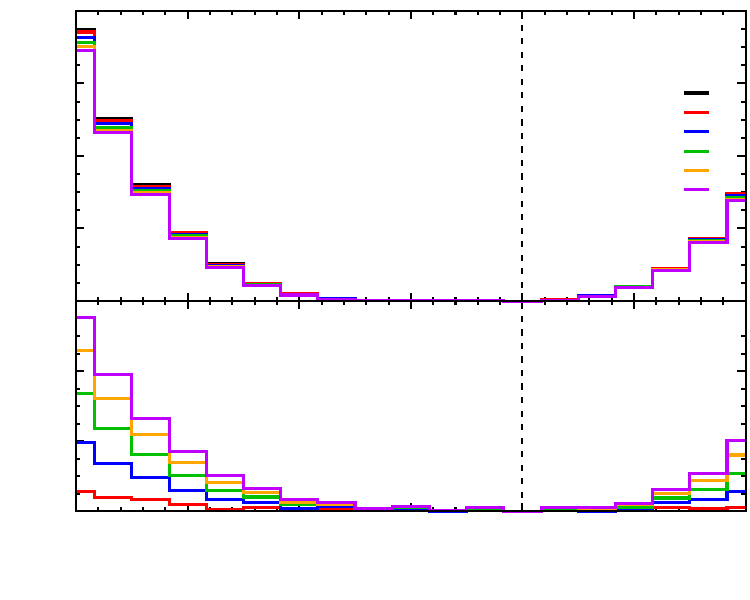
\includegraphics{pics/nuenorm_corr_chi2_S23}}%
    \gplfronttext
  \end{picture}%
\endgroup
}
	\resizebox{0.48\linewidth}{!}{% GNUPLOT: LaTeX picture with Postscript
\begingroup
  \makeatletter
  \providecommand\color[2][]{%
    \GenericError{(gnuplot) \space\space\space\@spaces}{%
      Package color not loaded in conjunction with
      terminal option `colourtext'%
    }{See the gnuplot documentation for explanation.%
    }{Either use 'blacktext' in gnuplot or load the package
      color.sty in LaTeX.}%
    \renewcommand\color[2][]{}%
  }%
  \providecommand\includegraphics[2][]{%
    \GenericError{(gnuplot) \space\space\space\@spaces}{%
      Package graphicx or graphics not loaded%
    }{See the gnuplot documentation for explanation.%
    }{The gnuplot epslatex terminal needs graphicx.sty or graphics.sty.}%
    \renewcommand\includegraphics[2][]{}%
  }%
  \providecommand\rotatebox[2]{#2}%
  \@ifundefined{ifGPcolor}{%
    \newif\ifGPcolor
    \GPcolortrue
  }{}%
  \@ifundefined{ifGPblacktext}{%
    \newif\ifGPblacktext
    \GPblacktexttrue
  }{}%
  % define a \g@addto@macro without @ in the name:
  \let\gplgaddtomacro\g@addto@macro
  % define empty templates for all commands taking text:
  \gdef\gplbacktext{}%
  \gdef\gplfronttext{}%
  \makeatother
  \ifGPblacktext
    % no textcolor at all
    \def\colorrgb#1{}%
    \def\colorgray#1{}%
  \else
    % gray or color?
    \ifGPcolor
      \def\colorrgb#1{\color[rgb]{#1}}%
      \def\colorgray#1{\color[gray]{#1}}%
      \expandafter\def\csname LTw\endcsname{\color{white}}%
      \expandafter\def\csname LTb\endcsname{\color{black}}%
      \expandafter\def\csname LTa\endcsname{\color{black}}%
      \expandafter\def\csname LT0\endcsname{\color[rgb]{1,0,0}}%
      \expandafter\def\csname LT1\endcsname{\color[rgb]{0,1,0}}%
      \expandafter\def\csname LT2\endcsname{\color[rgb]{0,0,1}}%
      \expandafter\def\csname LT3\endcsname{\color[rgb]{1,0,1}}%
      \expandafter\def\csname LT4\endcsname{\color[rgb]{0,1,1}}%
      \expandafter\def\csname LT5\endcsname{\color[rgb]{1,1,0}}%
      \expandafter\def\csname LT6\endcsname{\color[rgb]{0,0,0}}%
      \expandafter\def\csname LT7\endcsname{\color[rgb]{1,0.3,0}}%
      \expandafter\def\csname LT8\endcsname{\color[rgb]{0.5,0.5,0.5}}%
    \else
      % gray
      \def\colorrgb#1{\color{black}}%
      \def\colorgray#1{\color[gray]{#1}}%
      \expandafter\def\csname LTw\endcsname{\color{white}}%
      \expandafter\def\csname LTb\endcsname{\color{black}}%
      \expandafter\def\csname LTa\endcsname{\color{black}}%
      \expandafter\def\csname LT0\endcsname{\color{black}}%
      \expandafter\def\csname LT1\endcsname{\color{black}}%
      \expandafter\def\csname LT2\endcsname{\color{black}}%
      \expandafter\def\csname LT3\endcsname{\color{black}}%
      \expandafter\def\csname LT4\endcsname{\color{black}}%
      \expandafter\def\csname LT5\endcsname{\color{black}}%
      \expandafter\def\csname LT6\endcsname{\color{black}}%
      \expandafter\def\csname LT7\endcsname{\color{black}}%
      \expandafter\def\csname LT8\endcsname{\color{black}}%
    \fi
  \fi
    \setlength{\unitlength}{0.0500bp}%
    \ifx\gptboxheight\undefined%
      \newlength{\gptboxheight}%
      \newlength{\gptboxwidth}%
      \newsavebox{\gptboxtext}%
    \fi%
    \setlength{\fboxrule}{0.5pt}%
    \setlength{\fboxsep}{1pt}%
\begin{picture}(10800.00,7560.00)%
    \gplgaddtomacro\gplbacktext{%
      \csname LTb\endcsname%%
      \put(870,799){\makebox(0,0)[r]{\strut{}0}}%
      \csname LTb\endcsname%%
      \put(870,1395){\makebox(0,0)[r]{\strut{}0.1}}%
      \csname LTb\endcsname%%
      \put(870,1992){\makebox(0,0)[r]{\strut{}0.2}}%
      \csname LTb\endcsname%%
      \put(870,2588){\makebox(0,0)[r]{\strut{}0.3}}%
      \csname LTb\endcsname%%
      \put(870,3184){\makebox(0,0)[r]{\strut{}0.4}}%
      \csname LTb\endcsname%%
      \put(1853,494){\makebox(0,0){\strut{}0.44}}%
      \csname LTb\endcsname%%
      \put(3110,494){\makebox(0,0){\strut{}0.46}}%
      \csname LTb\endcsname%%
      \put(4368,494){\makebox(0,0){\strut{}0.48}}%
      \csname LTb\endcsname%%
      \put(5626,494){\makebox(0,0){\strut{}0.5}}%
      \csname LTb\endcsname%%
      \put(6884,494){\makebox(0,0){\strut{}0.52}}%
      \csname LTb\endcsname%%
      \put(8142,494){\makebox(0,0){\strut{}0.54}}%
      \csname LTb\endcsname%%
      \put(9400,494){\makebox(0,0){\strut{}0.56}}%
    }%
    \gplgaddtomacro\gplfronttext{%
      \csname LTb\endcsname%%
      \put(378,2230){\rotatebox{-270}{\makebox(0,0){\strut{}$\Delta \chi^2 - \Delta \chi^2_0$}}}%
      \csname LTb\endcsname%%
      \put(5783,215){\makebox(0,0){\strut{}$\sin^2 \theta_{23}$}}%
      \csname LTb\endcsname%%
      \put(8240,2495){\makebox(0,0){\strut{}Difference}}%
      \csname LTb\endcsname%%
      \put(7767,2309){\makebox(0,0)[l]{\strut{}$1\%$}}%
      \csname LTb\endcsname%%
      \put(7767,2123){\makebox(0,0)[l]{\strut{}$2\%$}}%
      \csname LTb\endcsname%%
      \put(7767,1937){\makebox(0,0)[l]{\strut{}$3\%$}}%
      \csname LTb\endcsname%%
      \put(7767,1751){\makebox(0,0)[l]{\strut{}$4\%$}}%
      \csname LTb\endcsname%%
      \put(7767,1565){\makebox(0,0)[l]{\strut{}$5\%$}}%
    }%
    \gplgaddtomacro\gplbacktext{%
      \csname LTb\endcsname%%
      \put(870,3780){\makebox(0,0)[r]{\strut{}0}}%
      \csname LTb\endcsname%%
      \put(870,4242){\makebox(0,0)[r]{\strut{}50}}%
      \csname LTb\endcsname%%
      \put(870,4704){\makebox(0,0)[r]{\strut{}100}}%
      \csname LTb\endcsname%%
      \put(870,5166){\makebox(0,0)[r]{\strut{}150}}%
      \csname LTb\endcsname%%
      \put(870,5628){\makebox(0,0)[r]{\strut{}200}}%
      \csname LTb\endcsname%%
      \put(870,6090){\makebox(0,0)[r]{\strut{}250}}%
      \csname LTb\endcsname%%
      \put(870,6551){\makebox(0,0)[r]{\strut{}300}}%
      \csname LTb\endcsname%%
      \put(870,7013){\makebox(0,0)[r]{\strut{}350}}%
      \csname LTb\endcsname%%
      \put(1853,3594){\makebox(0,0){\strut{}}}%
      \csname LTb\endcsname%%
      \put(3110,3594){\makebox(0,0){\strut{}}}%
      \csname LTb\endcsname%%
      \put(4368,3594){\makebox(0,0){\strut{}}}%
      \csname LTb\endcsname%%
      \put(5626,3594){\makebox(0,0){\strut{}}}%
      \csname LTb\endcsname%%
      \put(6884,3594){\makebox(0,0){\strut{}}}%
      \csname LTb\endcsname%%
      \put(8142,3594){\makebox(0,0){\strut{}}}%
      \csname LTb\endcsname%%
      \put(9400,3594){\makebox(0,0){\strut{}}}%
    }%
    \gplgaddtomacro\gplfronttext{%
      \csname LTb\endcsname%%
      \put(378,5623){\rotatebox{-270}{\makebox(0,0){\strut{}$\Delta \chi^2$}}}%
      \csname LTb\endcsname%%
      \put(5783,3538){\makebox(0,0){\strut{}}}%
      \csname LTb\endcsname%%
      \put(8240,7004){\makebox(0,0){\strut{}}}%
      \csname LTb\endcsname%%
      \put(7767,7004){\makebox(0,0)[l]{\strut{}No syst}}%
      \csname LTb\endcsname%%
      \put(7767,6818){\makebox(0,0)[l]{\strut{}$1\%$}}%
      \csname LTb\endcsname%%
      \put(7767,6632){\makebox(0,0)[l]{\strut{}$2\%$}}%
      \csname LTb\endcsname%%
      \put(7767,6446){\makebox(0,0)[l]{\strut{}$3\%$}}%
      \csname LTb\endcsname%%
      \put(7767,6260){\makebox(0,0)[l]{\strut{}$4\%$}}%
      \csname LTb\endcsname%%
      \put(7767,6074){\makebox(0,0)[l]{\strut{}$5\%$}}%
    }%
    \gplbacktext
    \put(0,0){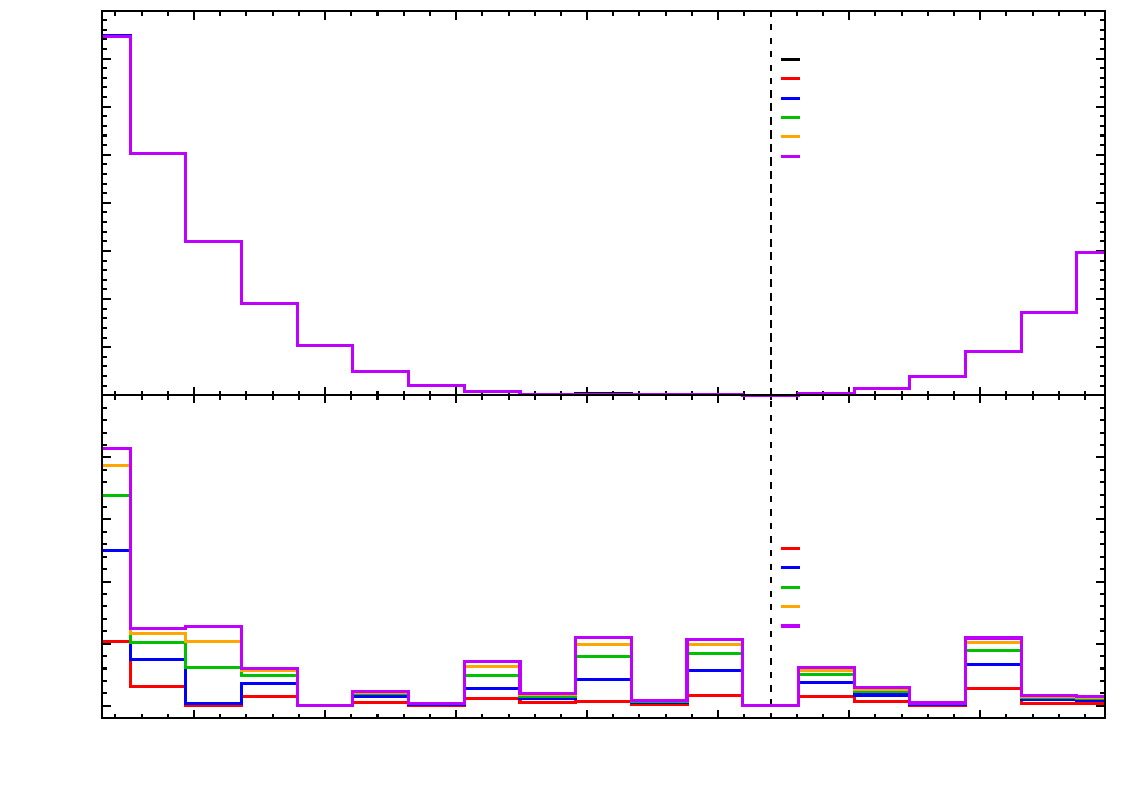
\includegraphics{nuenorm_anti_chi2_S23}}%
    \gplfronttext
  \end{picture}%
\endgroup
}
	\caption{$\chi^2$ profile for $sin^2 \theta_{23}$ for correlated (left) and anticorrelated (right) systematics. 
		The bottom panels show the difference of the different lines with the no systematic profile.}
	\label{fig:nuenorm_S23}
\end{figure}

\begin{figure}
	\centering
	\resizebox{0.48\linewidth}{!}{% GNUPLOT: LaTeX picture with Postscript
\begingroup
  \makeatletter
  \providecommand\color[2][]{%
    \GenericError{(gnuplot) \space\space\space\@spaces}{%
      Package color not loaded in conjunction with
      terminal option `colourtext'%
    }{See the gnuplot documentation for explanation.%
    }{Either use 'blacktext' in gnuplot or load the package
      color.sty in LaTeX.}%
    \renewcommand\color[2][]{}%
  }%
  \providecommand\includegraphics[2][]{%
    \GenericError{(gnuplot) \space\space\space\@spaces}{%
      Package graphicx or graphics not loaded%
    }{See the gnuplot documentation for explanation.%
    }{The gnuplot epslatex terminal needs graphicx.sty or graphics.sty.}%
    \renewcommand\includegraphics[2][]{}%
  }%
  \providecommand\rotatebox[2]{#2}%
  \@ifundefined{ifGPcolor}{%
    \newif\ifGPcolor
    \GPcolortrue
  }{}%
  \@ifundefined{ifGPblacktext}{%
    \newif\ifGPblacktext
    \GPblacktexttrue
  }{}%
  % define a \g@addto@macro without @ in the name:
  \let\gplgaddtomacro\g@addto@macro
  % define empty templates for all commands taking text:
  \gdef\gplbacktext{}%
  \gdef\gplfronttext{}%
  \makeatother
  \ifGPblacktext
    % no textcolor at all
    \def\colorrgb#1{}%
    \def\colorgray#1{}%
  \else
    % gray or color?
    \ifGPcolor
      \def\colorrgb#1{\color[rgb]{#1}}%
      \def\colorgray#1{\color[gray]{#1}}%
      \expandafter\def\csname LTw\endcsname{\color{white}}%
      \expandafter\def\csname LTb\endcsname{\color{black}}%
      \expandafter\def\csname LTa\endcsname{\color{black}}%
      \expandafter\def\csname LT0\endcsname{\color[rgb]{1,0,0}}%
      \expandafter\def\csname LT1\endcsname{\color[rgb]{0,1,0}}%
      \expandafter\def\csname LT2\endcsname{\color[rgb]{0,0,1}}%
      \expandafter\def\csname LT3\endcsname{\color[rgb]{1,0,1}}%
      \expandafter\def\csname LT4\endcsname{\color[rgb]{0,1,1}}%
      \expandafter\def\csname LT5\endcsname{\color[rgb]{1,1,0}}%
      \expandafter\def\csname LT6\endcsname{\color[rgb]{0,0,0}}%
      \expandafter\def\csname LT7\endcsname{\color[rgb]{1,0.3,0}}%
      \expandafter\def\csname LT8\endcsname{\color[rgb]{0.5,0.5,0.5}}%
    \else
      % gray
      \def\colorrgb#1{\color{black}}%
      \def\colorgray#1{\color[gray]{#1}}%
      \expandafter\def\csname LTw\endcsname{\color{white}}%
      \expandafter\def\csname LTb\endcsname{\color{black}}%
      \expandafter\def\csname LTa\endcsname{\color{black}}%
      \expandafter\def\csname LT0\endcsname{\color{black}}%
      \expandafter\def\csname LT1\endcsname{\color{black}}%
      \expandafter\def\csname LT2\endcsname{\color{black}}%
      \expandafter\def\csname LT3\endcsname{\color{black}}%
      \expandafter\def\csname LT4\endcsname{\color{black}}%
      \expandafter\def\csname LT5\endcsname{\color{black}}%
      \expandafter\def\csname LT6\endcsname{\color{black}}%
      \expandafter\def\csname LT7\endcsname{\color{black}}%
      \expandafter\def\csname LT8\endcsname{\color{black}}%
    \fi
  \fi
    \setlength{\unitlength}{0.0500bp}%
    \ifx\gptboxheight\undefined%
      \newlength{\gptboxheight}%
      \newlength{\gptboxwidth}%
      \newsavebox{\gptboxtext}%
    \fi%
    \setlength{\fboxrule}{0.5pt}%
    \setlength{\fboxsep}{1pt}%
\begin{picture}(7200.00,5760.00)%
    \gplgaddtomacro\gplbacktext{%
      \csname LTb\endcsname%%
      \put(747,927){\makebox(0,0)[r]{\strut{}2.47}}%
      \csname LTb\endcsname%%
      \put(747,1480){\makebox(0,0)[r]{\strut{}2.48}}%
      \csname LTb\endcsname%%
      \put(747,2033){\makebox(0,0)[r]{\strut{}2.49}}%
      \csname LTb\endcsname%%
      \put(747,2586){\makebox(0,0)[r]{\strut{}2.5}}%
      \csname LTb\endcsname%%
      \put(747,3139){\makebox(0,0)[r]{\strut{}2.51}}%
      \csname LTb\endcsname%%
      \put(747,3692){\makebox(0,0)[r]{\strut{}2.52}}%
      \csname LTb\endcsname%%
      \put(747,4246){\makebox(0,0)[r]{\strut{}2.53}}%
      \csname LTb\endcsname%%
      \put(747,4799){\makebox(0,0)[r]{\strut{}2.54}}%
      \csname LTb\endcsname%%
      \put(747,5352){\makebox(0,0)[r]{\strut{}2.55}}%
      \csname LTb\endcsname%%
      \put(1402,409){\makebox(0,0){\strut{}0.44}}%
      \csname LTb\endcsname%%
      \put(2192,409){\makebox(0,0){\strut{}0.46}}%
      \csname LTb\endcsname%%
      \put(2982,409){\makebox(0,0){\strut{}0.48}}%
      \csname LTb\endcsname%%
      \put(3772,409){\makebox(0,0){\strut{}0.5}}%
      \csname LTb\endcsname%%
      \put(4562,409){\makebox(0,0){\strut{}0.52}}%
      \csname LTb\endcsname%%
      \put(5352,409){\makebox(0,0){\strut{}0.54}}%
      \csname LTb\endcsname%%
      \put(6142,409){\makebox(0,0){\strut{}0.56}}%
      \csname LTb\endcsname%%
      \put(4915,3121){\makebox(0,0)[l]{\strut{}}}%
    }%
    \gplgaddtomacro\gplfronttext{%
      \csname LTb\endcsname%%
      \put(153,3084){\rotatebox{-270}{\makebox(0,0){\strut{}$\Delta m_{32}^2 / 10^{-3}$}}}%
      \csname LTb\endcsname%%
      \put(3871,130){\makebox(0,0){\strut{}$\sin^2 \theta_{23}$}}%
      \csname LTb\endcsname%%
      \put(6360,5406){\makebox(0,0)[r]{\strut{}No syst}}%
      \csname LTb\endcsname%%
      \put(6360,5220){\makebox(0,0)[r]{\strut{}1\,\%}}%
      \csname LTb\endcsname%%
      \put(6360,5034){\makebox(0,0)[r]{\strut{}2\,\%}}%
      \csname LTb\endcsname%%
      \put(6360,4848){\makebox(0,0)[r]{\strut{}3\,\%}}%
      \csname LTb\endcsname%%
      \put(6360,4662){\makebox(0,0)[r]{\strut{}4\,\%}}%
      \csname LTb\endcsname%%
      \put(6360,4476){\makebox(0,0)[r]{\strut{}5\,\%}}%
    }%
    \gplbacktext
    \put(0,0){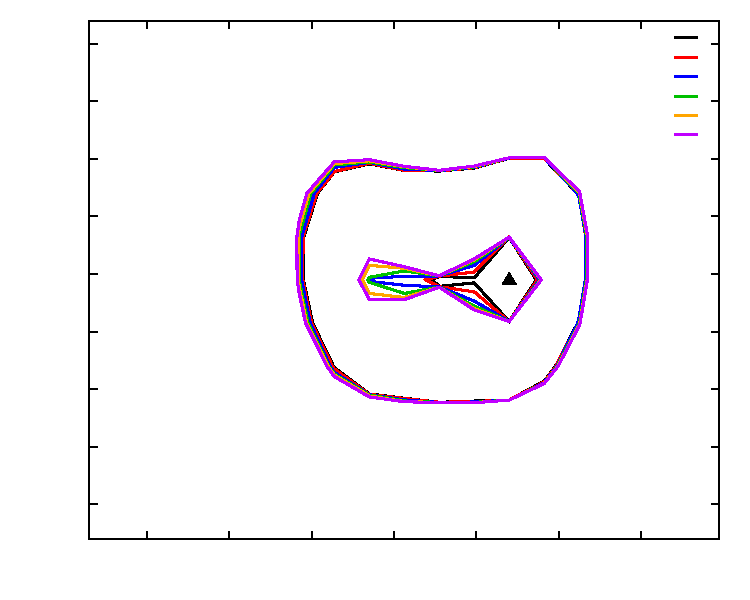
\includegraphics{pics/nuenorm_corr_cont_S23_M23}}%
    \gplfronttext
  \end{picture}%
\endgroup
}	%%%%%%%%%%%this is important
	\resizebox{0.48\linewidth}{!}{% GNUPLOT: LaTeX picture with Postscript
\begingroup
  \makeatletter
  \providecommand\color[2][]{%
    \GenericError{(gnuplot) \space\space\space\@spaces}{%
      Package color not loaded in conjunction with
      terminal option `colourtext'%
    }{See the gnuplot documentation for explanation.%
    }{Either use 'blacktext' in gnuplot or load the package
      color.sty in LaTeX.}%
    \renewcommand\color[2][]{}%
  }%
  \providecommand\includegraphics[2][]{%
    \GenericError{(gnuplot) \space\space\space\@spaces}{%
      Package graphicx or graphics not loaded%
    }{See the gnuplot documentation for explanation.%
    }{The gnuplot epslatex terminal needs graphicx.sty or graphics.sty.}%
    \renewcommand\includegraphics[2][]{}%
  }%
  \providecommand\rotatebox[2]{#2}%
  \@ifundefined{ifGPcolor}{%
    \newif\ifGPcolor
    \GPcolortrue
  }{}%
  \@ifundefined{ifGPblacktext}{%
    \newif\ifGPblacktext
    \GPblacktexttrue
  }{}%
  % define a \g@addto@macro without @ in the name:
  \let\gplgaddtomacro\g@addto@macro
  % define empty templates for all commands taking text:
  \gdef\gplbacktext{}%
  \gdef\gplfronttext{}%
  \makeatother
  \ifGPblacktext
    % no textcolor at all
    \def\colorrgb#1{}%
    \def\colorgray#1{}%
  \else
    % gray or color?
    \ifGPcolor
      \def\colorrgb#1{\color[rgb]{#1}}%
      \def\colorgray#1{\color[gray]{#1}}%
      \expandafter\def\csname LTw\endcsname{\color{white}}%
      \expandafter\def\csname LTb\endcsname{\color{black}}%
      \expandafter\def\csname LTa\endcsname{\color{black}}%
      \expandafter\def\csname LT0\endcsname{\color[rgb]{1,0,0}}%
      \expandafter\def\csname LT1\endcsname{\color[rgb]{0,1,0}}%
      \expandafter\def\csname LT2\endcsname{\color[rgb]{0,0,1}}%
      \expandafter\def\csname LT3\endcsname{\color[rgb]{1,0,1}}%
      \expandafter\def\csname LT4\endcsname{\color[rgb]{0,1,1}}%
      \expandafter\def\csname LT5\endcsname{\color[rgb]{1,1,0}}%
      \expandafter\def\csname LT6\endcsname{\color[rgb]{0,0,0}}%
      \expandafter\def\csname LT7\endcsname{\color[rgb]{1,0.3,0}}%
      \expandafter\def\csname LT8\endcsname{\color[rgb]{0.5,0.5,0.5}}%
    \else
      % gray
      \def\colorrgb#1{\color{black}}%
      \def\colorgray#1{\color[gray]{#1}}%
      \expandafter\def\csname LTw\endcsname{\color{white}}%
      \expandafter\def\csname LTb\endcsname{\color{black}}%
      \expandafter\def\csname LTa\endcsname{\color{black}}%
      \expandafter\def\csname LT0\endcsname{\color{black}}%
      \expandafter\def\csname LT1\endcsname{\color{black}}%
      \expandafter\def\csname LT2\endcsname{\color{black}}%
      \expandafter\def\csname LT3\endcsname{\color{black}}%
      \expandafter\def\csname LT4\endcsname{\color{black}}%
      \expandafter\def\csname LT5\endcsname{\color{black}}%
      \expandafter\def\csname LT6\endcsname{\color{black}}%
      \expandafter\def\csname LT7\endcsname{\color{black}}%
      \expandafter\def\csname LT8\endcsname{\color{black}}%
    \fi
  \fi
    \setlength{\unitlength}{0.0500bp}%
    \ifx\gptboxheight\undefined%
      \newlength{\gptboxheight}%
      \newlength{\gptboxwidth}%
      \newsavebox{\gptboxtext}%
    \fi%
    \setlength{\fboxrule}{0.5pt}%
    \setlength{\fboxsep}{1pt}%
\begin{picture}(10800.00,7560.00)%
    \gplgaddtomacro\gplbacktext{%
      \csname LTb\endcsname%%
      \put(747,1047){\makebox(0,0)[r]{\strut{}2.47}}%
      \csname LTb\endcsname%%
      \put(747,1800){\makebox(0,0)[r]{\strut{}2.48}}%
      \csname LTb\endcsname%%
      \put(747,2553){\makebox(0,0)[r]{\strut{}2.49}}%
      \csname LTb\endcsname%%
      \put(747,3306){\makebox(0,0)[r]{\strut{}2.5}}%
      \csname LTb\endcsname%%
      \put(747,4059){\makebox(0,0)[r]{\strut{}2.51}}%
      \csname LTb\endcsname%%
      \put(747,4812){\makebox(0,0)[r]{\strut{}2.52}}%
      \csname LTb\endcsname%%
      \put(747,5566){\makebox(0,0)[r]{\strut{}2.53}}%
      \csname LTb\endcsname%%
      \put(747,6319){\makebox(0,0)[r]{\strut{}2.54}}%
      \csname LTb\endcsname%%
      \put(747,7072){\makebox(0,0)[r]{\strut{}2.55}}%
      \csname LTb\endcsname%%
      \put(1731,409){\makebox(0,0){\strut{}0.44}}%
      \csname LTb\endcsname%%
      \put(2992,409){\makebox(0,0){\strut{}0.46}}%
      \csname LTb\endcsname%%
      \put(4253,409){\makebox(0,0){\strut{}0.48}}%
      \csname LTb\endcsname%%
      \put(5513,409){\makebox(0,0){\strut{}0.5}}%
      \csname LTb\endcsname%%
      \put(6774,409){\makebox(0,0){\strut{}0.52}}%
      \csname LTb\endcsname%%
      \put(8035,409){\makebox(0,0){\strut{}0.54}}%
      \csname LTb\endcsname%%
      \put(9295,409){\makebox(0,0){\strut{}0.56}}%
      \csname LTb\endcsname%%
      \put(7315,4021){\makebox(0,0)[l]{\strut{}}}%
    }%
    \gplgaddtomacro\gplfronttext{%
      \csname LTb\endcsname%%
      \put(153,3984){\rotatebox{-270}{\makebox(0,0){\strut{}$\Delta m_{32}^2 / 10^{-3}$}}}%
      \csname LTb\endcsname%%
      \put(5671,130){\makebox(0,0){\strut{}$\sin^2 \theta_{23}$}}%
      \csname LTb\endcsname%%
      \put(9705,7206){\makebox(0,0)[r]{\strut{}No syst}}%
      \csname LTb\endcsname%%
      \put(9705,7020){\makebox(0,0)[r]{\strut{}$1\%$}}%
      \csname LTb\endcsname%%
      \put(9705,6834){\makebox(0,0)[r]{\strut{}$2\%$}}%
      \csname LTb\endcsname%%
      \put(9705,6648){\makebox(0,0)[r]{\strut{}$3\%$}}%
      \csname LTb\endcsname%%
      \put(9705,6462){\makebox(0,0)[r]{\strut{}$4\%$}}%
      \csname LTb\endcsname%%
      \put(9705,6276){\makebox(0,0)[r]{\strut{}$5\%$}}%
    }%
    \gplbacktext
    \put(0,0){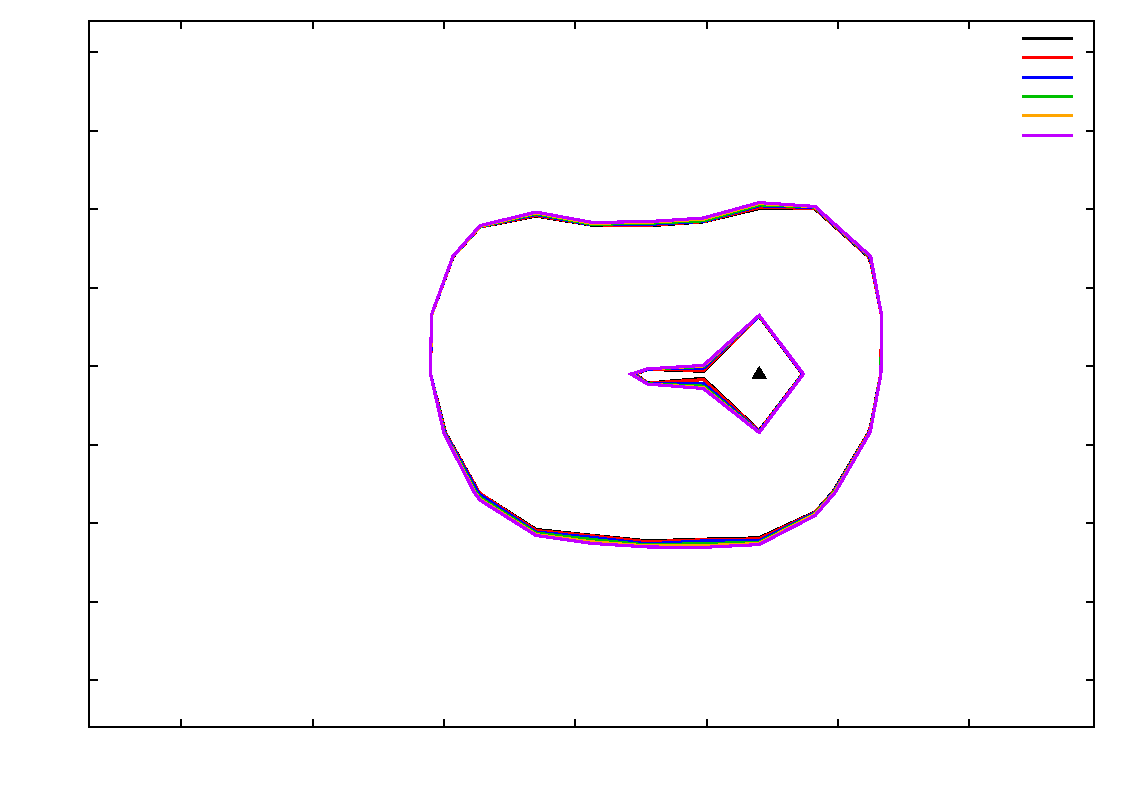
\includegraphics{nuenorm_anti_cont_S23_M23}}%
    \gplfronttext
  \end{picture}%
\endgroup
}
	\caption{Contour plot of the $\chi^2$ profile for $\Delta m_{23}^2$ vs.\  $sin^2 \theta_{23}$ %
		for correlated (left) and anticorrelated (right) systematics. 
		The inner contour and outer contour corresponds respectively to the $1\sigma$ and $3\sigma$ %
		contour lines.}
	\label{fig:nuenorm_S23_M23}
\end{figure}

\begin{figure}
	\centering
	\resizebox{0.48\linewidth}{!}{% GNUPLOT: LaTeX picture with Postscript
\begingroup
  \makeatletter
  \providecommand\color[2][]{%
    \GenericError{(gnuplot) \space\space\space\@spaces}{%
      Package color not loaded in conjunction with
      terminal option `colourtext'%
    }{See the gnuplot documentation for explanation.%
    }{Either use 'blacktext' in gnuplot or load the package
      color.sty in LaTeX.}%
    \renewcommand\color[2][]{}%
  }%
  \providecommand\includegraphics[2][]{%
    \GenericError{(gnuplot) \space\space\space\@spaces}{%
      Package graphicx or graphics not loaded%
    }{See the gnuplot documentation for explanation.%
    }{The gnuplot epslatex terminal needs graphicx.sty or graphics.sty.}%
    \renewcommand\includegraphics[2][]{}%
  }%
  \providecommand\rotatebox[2]{#2}%
  \@ifundefined{ifGPcolor}{%
    \newif\ifGPcolor
    \GPcolortrue
  }{}%
  \@ifundefined{ifGPblacktext}{%
    \newif\ifGPblacktext
    \GPblacktexttrue
  }{}%
  % define a \g@addto@macro without @ in the name:
  \let\gplgaddtomacro\g@addto@macro
  % define empty templates for all commands taking text:
  \gdef\gplbacktext{}%
  \gdef\gplfronttext{}%
  \makeatother
  \ifGPblacktext
    % no textcolor at all
    \def\colorrgb#1{}%
    \def\colorgray#1{}%
  \else
    % gray or color?
    \ifGPcolor
      \def\colorrgb#1{\color[rgb]{#1}}%
      \def\colorgray#1{\color[gray]{#1}}%
      \expandafter\def\csname LTw\endcsname{\color{white}}%
      \expandafter\def\csname LTb\endcsname{\color{black}}%
      \expandafter\def\csname LTa\endcsname{\color{black}}%
      \expandafter\def\csname LT0\endcsname{\color[rgb]{1,0,0}}%
      \expandafter\def\csname LT1\endcsname{\color[rgb]{0,1,0}}%
      \expandafter\def\csname LT2\endcsname{\color[rgb]{0,0,1}}%
      \expandafter\def\csname LT3\endcsname{\color[rgb]{1,0,1}}%
      \expandafter\def\csname LT4\endcsname{\color[rgb]{0,1,1}}%
      \expandafter\def\csname LT5\endcsname{\color[rgb]{1,1,0}}%
      \expandafter\def\csname LT6\endcsname{\color[rgb]{0,0,0}}%
      \expandafter\def\csname LT7\endcsname{\color[rgb]{1,0.3,0}}%
      \expandafter\def\csname LT8\endcsname{\color[rgb]{0.5,0.5,0.5}}%
    \else
      % gray
      \def\colorrgb#1{\color{black}}%
      \def\colorgray#1{\color[gray]{#1}}%
      \expandafter\def\csname LTw\endcsname{\color{white}}%
      \expandafter\def\csname LTb\endcsname{\color{black}}%
      \expandafter\def\csname LTa\endcsname{\color{black}}%
      \expandafter\def\csname LT0\endcsname{\color{black}}%
      \expandafter\def\csname LT1\endcsname{\color{black}}%
      \expandafter\def\csname LT2\endcsname{\color{black}}%
      \expandafter\def\csname LT3\endcsname{\color{black}}%
      \expandafter\def\csname LT4\endcsname{\color{black}}%
      \expandafter\def\csname LT5\endcsname{\color{black}}%
      \expandafter\def\csname LT6\endcsname{\color{black}}%
      \expandafter\def\csname LT7\endcsname{\color{black}}%
      \expandafter\def\csname LT8\endcsname{\color{black}}%
    \fi
  \fi
    \setlength{\unitlength}{0.0500bp}%
    \ifx\gptboxheight\undefined%
      \newlength{\gptboxheight}%
      \newlength{\gptboxwidth}%
      \newsavebox{\gptboxtext}%
    \fi%
    \setlength{\fboxrule}{0.5pt}%
    \setlength{\fboxsep}{1pt}%
\begin{picture}(11520.00,6540.00)%
    \gplgaddtomacro\gplbacktext{%
      \csname LTb\endcsname%%
      \put(543,595){\makebox(0,0)[r]{\strut{}0}}%
      \csname LTb\endcsname%%
      \put(543,1555){\makebox(0,0)[r]{\strut{}2}}%
      \csname LTb\endcsname%%
      \put(543,2514){\makebox(0,0)[r]{\strut{}4}}%
      \csname LTb\endcsname%%
      \put(543,3474){\makebox(0,0)[r]{\strut{}6}}%
      \csname LTb\endcsname%%
      \put(543,4434){\makebox(0,0)[r]{\strut{}8}}%
      \csname LTb\endcsname%%
      \put(543,5393){\makebox(0,0)[r]{\strut{}10}}%
      \csname LTb\endcsname%%
      \put(543,6353){\makebox(0,0)[r]{\strut{}12}}%
      \csname LTb\endcsname%%
      \put(883,409){\makebox(0,0){\strut{}-1.0$\pi$}}%
      \csname LTb\endcsname%%
      \put(2565,409){\makebox(0,0){\strut{}-0.6$\pi$}}%
      \csname LTb\endcsname%%
      \put(4247,409){\makebox(0,0){\strut{}-0.3$\pi$}}%
      \csname LTb\endcsname%%
      \put(5929,409){\makebox(0,0){\strut{}0.0$\pi$}}%
      \csname LTb\endcsname%%
      \put(7611,409){\makebox(0,0){\strut{}0.3$\pi$}}%
      \csname LTb\endcsname%%
      \put(9293,409){\makebox(0,0){\strut{}0.6$\pi$}}%
      \csname LTb\endcsname%%
      \put(10975,409){\makebox(0,0){\strut{}1.0$\pi$}}%
      \csname LTb\endcsname%%
      \put(5929,3234){\makebox(0,0){\strut{}$5 \sigma$}}%
      \csname LTb\endcsname%%
      \put(5929,2274){\makebox(0,0){\strut{}$3 \sigma$}}%
    }%
    \gplgaddtomacro\gplfronttext{%
      \csname LTb\endcsname%%
      \put(153,3474){\rotatebox{-270}{\makebox(0,0){\strut{}$\sigma (\delta_\text{CP})$}}}%
      \csname LTb\endcsname%%
      \put(5929,130){\makebox(0,0){\strut{}$\delta_\text{CP}$}}%
      \csname LTb\endcsname%%
      \put(1178,6186){\makebox(0,0)[l]{\strut{}No syst}}%
      \csname LTb\endcsname%%
      \put(1178,6000){\makebox(0,0)[l]{\strut{}$1\%$}}%
      \csname LTb\endcsname%%
      \put(1178,5814){\makebox(0,0)[l]{\strut{}$2\%$}}%
      \csname LTb\endcsname%%
      \put(1178,5628){\makebox(0,0)[l]{\strut{}$3\%$}}%
      \csname LTb\endcsname%%
      \put(1178,5442){\makebox(0,0)[l]{\strut{}$4\%$}}%
      \csname LTb\endcsname%%
      \put(1178,5256){\makebox(0,0)[l]{\strut{}$5\%$}}%
    }%
    \gplbacktext
    \put(0,0){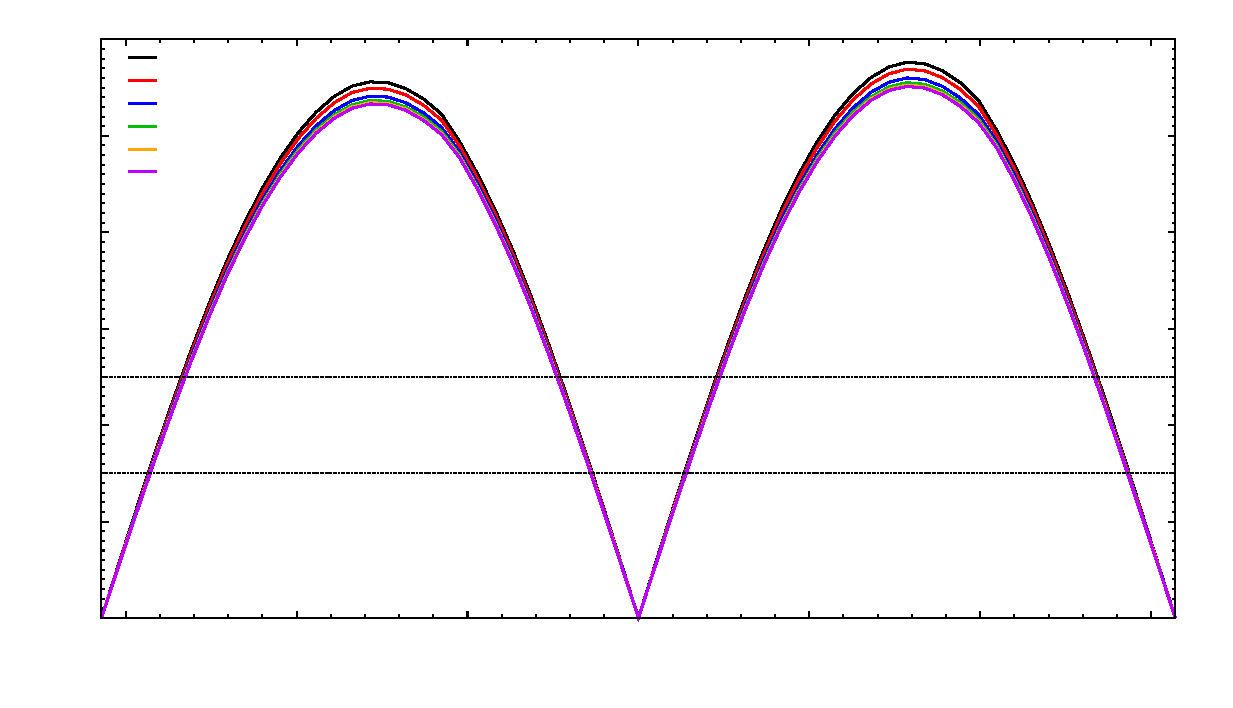
\includegraphics{pics/nuenorm_corr_sensitivity}}%
    \gplfronttext
  \end{picture}%
\endgroup
}
	\resizebox{0.48\linewidth}{!}{% GNUPLOT: LaTeX picture with Postscript
\begingroup
  \makeatletter
  \providecommand\color[2][]{%
    \GenericError{(gnuplot) \space\space\space\@spaces}{%
      Package color not loaded in conjunction with
      terminal option `colourtext'%
    }{See the gnuplot documentation for explanation.%
    }{Either use 'blacktext' in gnuplot or load the package
      color.sty in LaTeX.}%
    \renewcommand\color[2][]{}%
  }%
  \providecommand\includegraphics[2][]{%
    \GenericError{(gnuplot) \space\space\space\@spaces}{%
      Package graphicx or graphics not loaded%
    }{See the gnuplot documentation for explanation.%
    }{The gnuplot epslatex terminal needs graphicx.sty or graphics.sty.}%
    \renewcommand\includegraphics[2][]{}%
  }%
  \providecommand\rotatebox[2]{#2}%
  \@ifundefined{ifGPcolor}{%
    \newif\ifGPcolor
    \GPcolortrue
  }{}%
  \@ifundefined{ifGPblacktext}{%
    \newif\ifGPblacktext
    \GPblacktexttrue
  }{}%
  % define a \g@addto@macro without @ in the name:
  \let\gplgaddtomacro\g@addto@macro
  % define empty templates for all commands taking text:
  \gdef\gplbacktext{}%
  \gdef\gplfronttext{}%
  \makeatother
  \ifGPblacktext
    % no textcolor at all
    \def\colorrgb#1{}%
    \def\colorgray#1{}%
  \else
    % gray or color?
    \ifGPcolor
      \def\colorrgb#1{\color[rgb]{#1}}%
      \def\colorgray#1{\color[gray]{#1}}%
      \expandafter\def\csname LTw\endcsname{\color{white}}%
      \expandafter\def\csname LTb\endcsname{\color{black}}%
      \expandafter\def\csname LTa\endcsname{\color{black}}%
      \expandafter\def\csname LT0\endcsname{\color[rgb]{1,0,0}}%
      \expandafter\def\csname LT1\endcsname{\color[rgb]{0,1,0}}%
      \expandafter\def\csname LT2\endcsname{\color[rgb]{0,0,1}}%
      \expandafter\def\csname LT3\endcsname{\color[rgb]{1,0,1}}%
      \expandafter\def\csname LT4\endcsname{\color[rgb]{0,1,1}}%
      \expandafter\def\csname LT5\endcsname{\color[rgb]{1,1,0}}%
      \expandafter\def\csname LT6\endcsname{\color[rgb]{0,0,0}}%
      \expandafter\def\csname LT7\endcsname{\color[rgb]{1,0.3,0}}%
      \expandafter\def\csname LT8\endcsname{\color[rgb]{0.5,0.5,0.5}}%
    \else
      % gray
      \def\colorrgb#1{\color{black}}%
      \def\colorgray#1{\color[gray]{#1}}%
      \expandafter\def\csname LTw\endcsname{\color{white}}%
      \expandafter\def\csname LTb\endcsname{\color{black}}%
      \expandafter\def\csname LTa\endcsname{\color{black}}%
      \expandafter\def\csname LT0\endcsname{\color{black}}%
      \expandafter\def\csname LT1\endcsname{\color{black}}%
      \expandafter\def\csname LT2\endcsname{\color{black}}%
      \expandafter\def\csname LT3\endcsname{\color{black}}%
      \expandafter\def\csname LT4\endcsname{\color{black}}%
      \expandafter\def\csname LT5\endcsname{\color{black}}%
      \expandafter\def\csname LT6\endcsname{\color{black}}%
      \expandafter\def\csname LT7\endcsname{\color{black}}%
      \expandafter\def\csname LT8\endcsname{\color{black}}%
    \fi
  \fi
    \setlength{\unitlength}{0.0500bp}%
    \ifx\gptboxheight\undefined%
      \newlength{\gptboxheight}%
      \newlength{\gptboxwidth}%
      \newsavebox{\gptboxtext}%
    \fi%
    \setlength{\fboxrule}{0.5pt}%
    \setlength{\fboxsep}{1pt}%
\begin{picture}(7200.00,5040.00)%
    \gplgaddtomacro\gplbacktext{%
      \csname LTb\endcsname%%
      \put(543,595){\makebox(0,0)[r]{\strut{}0}}%
      \csname LTb\endcsname%%
      \put(543,1305){\makebox(0,0)[r]{\strut{}2}}%
      \csname LTb\endcsname%%
      \put(543,2014){\makebox(0,0)[r]{\strut{}4}}%
      \csname LTb\endcsname%%
      \put(543,2724){\makebox(0,0)[r]{\strut{}6}}%
      \csname LTb\endcsname%%
      \put(543,3434){\makebox(0,0)[r]{\strut{}8}}%
      \csname LTb\endcsname%%
      \put(543,4143){\makebox(0,0)[r]{\strut{}10}}%
      \csname LTb\endcsname%%
      \put(543,4853){\makebox(0,0)[r]{\strut{}12}}%
      \csname LTb\endcsname%%
      \put(645,409){\makebox(0,0){\strut{}-1.0$\pi$}}%
      \csname LTb\endcsname%%
      \put(1426,409){\makebox(0,0){\strut{}-0.8$\pi$}}%
      \csname LTb\endcsname%%
      \put(2207,409){\makebox(0,0){\strut{}-0.5$\pi$}}%
      \csname LTb\endcsname%%
      \put(2988,409){\makebox(0,0){\strut{}-0.2$\pi$}}%
      \csname LTb\endcsname%%
      \put(3769,409){\makebox(0,0){\strut{}0.0$\pi$}}%
      \csname LTb\endcsname%%
      \put(4550,409){\makebox(0,0){\strut{}0.2$\pi$}}%
      \csname LTb\endcsname%%
      \put(5331,409){\makebox(0,0){\strut{}0.5$\pi$}}%
      \csname LTb\endcsname%%
      \put(6112,409){\makebox(0,0){\strut{}0.8$\pi$}}%
      \csname LTb\endcsname%%
      \put(6893,409){\makebox(0,0){\strut{}1.0$\pi$}}%
      \csname LTb\endcsname%%
      \put(3769,2547){\makebox(0,0){\strut{}$5 \sigma$}}%
      \csname LTb\endcsname%%
      \put(3769,1837){\makebox(0,0){\strut{}$3 \sigma$}}%
    }%
    \gplgaddtomacro\gplfronttext{%
      \csname LTb\endcsname%%
      \put(153,2724){\rotatebox{-270}{\makebox(0,0){\strut{}$\sigma (\delta_\text{CP})$}}}%
      \csname LTb\endcsname%%
      \put(3769,130){\makebox(0,0){\strut{}$\delta_\text{CP}$}}%
      \csname LTb\endcsname%%
      \put(1178,4686){\makebox(0,0)[l]{\strut{}No syst}}%
      \csname LTb\endcsname%%
      \put(1178,4500){\makebox(0,0)[l]{\strut{}1\,\%}}%
      \csname LTb\endcsname%%
      \put(1178,4314){\makebox(0,0)[l]{\strut{}2\,\%}}%
      \csname LTb\endcsname%%
      \put(1178,4128){\makebox(0,0)[l]{\strut{}3\,\%}}%
      \csname LTb\endcsname%%
      \put(1178,3942){\makebox(0,0)[l]{\strut{}4\,\%}}%
      \csname LTb\endcsname%%
      \put(1178,3756){\makebox(0,0)[l]{\strut{}5\,\%}}%
    }%
    \gplbacktext
    \put(0,0){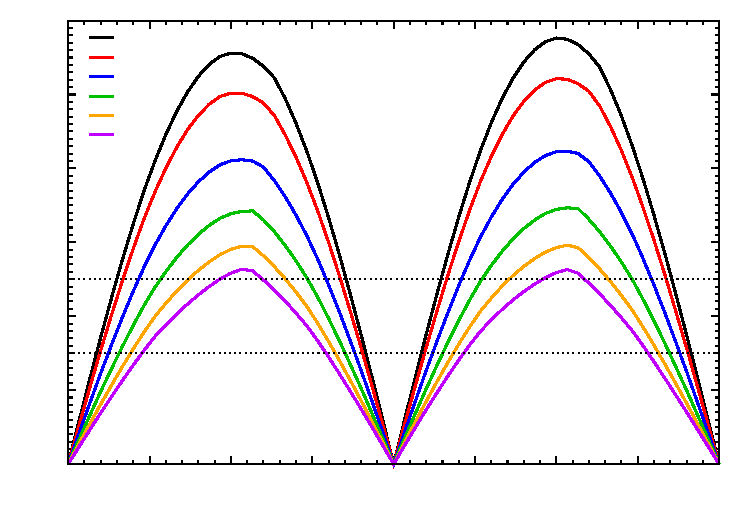
\includegraphics{pics/nuenorm_anti_sensitivity}}%
    \gplfronttext
  \end{picture}%
\endgroup
}
	\caption{Expected signifcance to exclude $\sin\delta_\text{CP} = 0$ for correlated (left) and anticorrelated (right) systematics.
		The anticorrelation between the $\nu_e$ and $\cj{\nu}_e$ CC cross-section systematic errors %
       		masks the resolution power to distinguihsing neutrino from anti-neutrino events. }
	\label{fig:nuenorm_sensitivity}
\end{figure}



\subsection{Variations of the nominal model}

\begin{table}
	\centering
	\caption{Variations of the nominal systematic model, labelled \textbf{0}.
		The second column speficy the modification applied to the reference model:
		the sets in the first block have one or more parameters added, %
		whereas one or more parameters are removed in the variations of the second block.
		The systematic models in the last group have the same number of parameters of the nominal model, %
		with the modifications speficied.}
	\label{tab:variations}
	\begin{tabular}{rr@{\quad}l}
		\toprule
		%Label		& & Modification \\
		%\midrule
		\textbf{0}	& 	& Nominal T2K model \\
		\midrule
		\textbf{1a}	& $=\quad\bs{0}\quad+$ 	& $\nu_e$ CC cross-sections for $0.1\,\text{GeV} < E_\text{true} < 0.6\,\text{GeV}$ \\
		\textbf{1b}	& $=\quad\bs{0}\quad+$ 	& $\nu_e$ CC cross-sections for $0.6\,\text{GeV} < E_\text{true} < 1.0\,\text{GeV}$ \\
		\textbf{2a}	& $=\quad\bs{0}\quad+$ 	& $\cj{\nu}_e$ CC cross-sections for $0.1\,\text{GeV} < E_\text{true} < 0.6\,\text{GeV}$ \\
		\textbf{2b}	& $=\quad\bs{0}\quad+$ 	& $\cj{\nu}_e$ CC cross-sections for $0.6\,\text{GeV} < E_\text{true} < 1.0\,\text{GeV}$ \\
		\textbf{9}	& $=\quad\bs{0}\quad+$	& CC1$\pi^\pm$ and CC-coh cross-sections for $\nu_e$ and $\cj{\nu}_e$. \\
		\textbf{10}	& $=\quad\bs{0}\quad+$	& CC1$\pi^\pm$ and CC-coh cross-sections for $\nu_\mu$ and $\cj{\nu}_\mu$ \\
				&   			  & \hfill	for $2\,\text{GeV} < E_\text{true} < 10\,\text{GeV}$ \\
		\midrule
		\textbf{6a}	& $=\quad\bs{0}\quad-$	& $\nu$ 2p2h normalisation \\
		\textbf{7a}	& $=\quad\bs{0}\quad-$	& $\cj{\nu}$ 2p2h normalisation \\
		\textbf{67}	& $=\quad\bs{0}\quad-$	& $\nu$ and $\cj{\nu}$ 2p2h normalisation \\
		\midrule
		\textbf{8}	& $=\quad\bs{0}\quad\times$	& increased $\nu_e$ flux uncertainty in $\nu$-mode beam (2\%) \\
		\textbf{11a}	& $=\quad\bs{0}\quad\times$	& increased SK energy scale (2.4\% $\to$ 2.9\%) \\
		\textbf{11b}	& $=\quad\bs{0}\quad\times$	& decreased SK energy scale (2.4\% $\to$ 1.9\%) \\
		\textbf{flux}	& $=\quad\bs{0}\quad\times$	& flux model additions from INGRID studies \\
		\bottomrule
	\end{tabular}
\end{table}


A series of modifications are performed on the nominal systematic and new systematic sets are created.
Performing a sensitivity study with these variations of the nominal model, we can determine %
if certain systematic errors needs more control than other.
All of the produced sets are listed in \reftab{tab:variations}, however only a subset is discussed in this work %
and these are the the sets labelled \textbf{8}, \textbf{11a}, and \textbf{11b} (see \reftab{tab:variations} %
for the meaning of the labels).
The remaining ones will be studied in the future.

\begin{figure}
	\centering
	\resizebox{0.48\linewidth}{!}{% GNUPLOT: LaTeX picture with Postscript
\begingroup
  \makeatletter
  \providecommand\color[2][]{%
    \GenericError{(gnuplot) \space\space\space\@spaces}{%
      Package color not loaded in conjunction with
      terminal option `colourtext'%
    }{See the gnuplot documentation for explanation.%
    }{Either use 'blacktext' in gnuplot or load the package
      color.sty in LaTeX.}%
    \renewcommand\color[2][]{}%
  }%
  \providecommand\includegraphics[2][]{%
    \GenericError{(gnuplot) \space\space\space\@spaces}{%
      Package graphicx or graphics not loaded%
    }{See the gnuplot documentation for explanation.%
    }{The gnuplot epslatex terminal needs graphicx.sty or graphics.sty.}%
    \renewcommand\includegraphics[2][]{}%
  }%
  \providecommand\rotatebox[2]{#2}%
  \@ifundefined{ifGPcolor}{%
    \newif\ifGPcolor
    \GPcolortrue
  }{}%
  \@ifundefined{ifGPblacktext}{%
    \newif\ifGPblacktext
    \GPblacktexttrue
  }{}%
  % define a \g@addto@macro without @ in the name:
  \let\gplgaddtomacro\g@addto@macro
  % define empty templates for all commands taking text:
  \gdef\gplbacktext{}%
  \gdef\gplfronttext{}%
  \makeatother
  \ifGPblacktext
    % no textcolor at all
    \def\colorrgb#1{}%
    \def\colorgray#1{}%
  \else
    % gray or color?
    \ifGPcolor
      \def\colorrgb#1{\color[rgb]{#1}}%
      \def\colorgray#1{\color[gray]{#1}}%
      \expandafter\def\csname LTw\endcsname{\color{white}}%
      \expandafter\def\csname LTb\endcsname{\color{black}}%
      \expandafter\def\csname LTa\endcsname{\color{black}}%
      \expandafter\def\csname LT0\endcsname{\color[rgb]{1,0,0}}%
      \expandafter\def\csname LT1\endcsname{\color[rgb]{0,1,0}}%
      \expandafter\def\csname LT2\endcsname{\color[rgb]{0,0,1}}%
      \expandafter\def\csname LT3\endcsname{\color[rgb]{1,0,1}}%
      \expandafter\def\csname LT4\endcsname{\color[rgb]{0,1,1}}%
      \expandafter\def\csname LT5\endcsname{\color[rgb]{1,1,0}}%
      \expandafter\def\csname LT6\endcsname{\color[rgb]{0,0,0}}%
      \expandafter\def\csname LT7\endcsname{\color[rgb]{1,0.3,0}}%
      \expandafter\def\csname LT8\endcsname{\color[rgb]{0.5,0.5,0.5}}%
    \else
      % gray
      \def\colorrgb#1{\color{black}}%
      \def\colorgray#1{\color[gray]{#1}}%
      \expandafter\def\csname LTw\endcsname{\color{white}}%
      \expandafter\def\csname LTb\endcsname{\color{black}}%
      \expandafter\def\csname LTa\endcsname{\color{black}}%
      \expandafter\def\csname LT0\endcsname{\color{black}}%
      \expandafter\def\csname LT1\endcsname{\color{black}}%
      \expandafter\def\csname LT2\endcsname{\color{black}}%
      \expandafter\def\csname LT3\endcsname{\color{black}}%
      \expandafter\def\csname LT4\endcsname{\color{black}}%
      \expandafter\def\csname LT5\endcsname{\color{black}}%
      \expandafter\def\csname LT6\endcsname{\color{black}}%
      \expandafter\def\csname LT7\endcsname{\color{black}}%
      \expandafter\def\csname LT8\endcsname{\color{black}}%
    \fi
  \fi
    \setlength{\unitlength}{0.0500bp}%
    \ifx\gptboxheight\undefined%
      \newlength{\gptboxheight}%
      \newlength{\gptboxwidth}%
      \newsavebox{\gptboxtext}%
    \fi%
    \setlength{\fboxrule}{0.5pt}%
    \setlength{\fboxsep}{1pt}%
\begin{picture}(10800.00,7560.00)%
    \gplgaddtomacro\gplbacktext{%
      \csname LTb\endcsname%%
      \put(870,680){\makebox(0,0)[r]{\strut{}-0.3}}%
      \csname LTb\endcsname%%
      \put(870,1300){\makebox(0,0)[r]{\strut{}-0.2}}%
      \csname LTb\endcsname%%
      \put(870,1920){\makebox(0,0)[r]{\strut{}-0.1}}%
      \csname LTb\endcsname%%
      \put(870,2540){\makebox(0,0)[r]{\strut{}0}}%
      \csname LTb\endcsname%%
      \put(870,3160){\makebox(0,0)[r]{\strut{}0.1}}%
      \csname LTb\endcsname%%
      \put(972,494){\makebox(0,0){\strut{}-1.00$\pi$}}%
      \csname LTb\endcsname%%
      \put(1934,494){\makebox(0,0){\strut{}-0.80$\pi$}}%
      \csname LTb\endcsname%%
      \put(2897,494){\makebox(0,0){\strut{}-0.60$\pi$}}%
      \csname LTb\endcsname%%
      \put(3859,494){\makebox(0,0){\strut{}-0.40$\pi$}}%
      \csname LTb\endcsname%%
      \put(4821,494){\makebox(0,0){\strut{}-0.20$\pi$}}%
      \csname LTb\endcsname%%
      \put(5784,494){\makebox(0,0){\strut{}0.00$\pi$}}%
      \csname LTb\endcsname%%
      \put(6746,494){\makebox(0,0){\strut{}0.20$\pi$}}%
      \csname LTb\endcsname%%
      \put(7708,494){\makebox(0,0){\strut{}0.40$\pi$}}%
      \csname LTb\endcsname%%
      \put(8670,494){\makebox(0,0){\strut{}0.60$\pi$}}%
      \csname LTb\endcsname%%
      \put(9633,494){\makebox(0,0){\strut{}0.80$\pi$}}%
      \csname LTb\endcsname%%
      \put(10595,494){\makebox(0,0){\strut{}1.00$\pi$}}%
    }%
    \gplgaddtomacro\gplfronttext{%
      \csname LTb\endcsname%%
      \put(276,2230){\rotatebox{-270}{\makebox(0,0){\strut{}$\Delta \chi^2 - \Delta \chi^2_0$}}}%
      \csname LTb\endcsname%%
      \put(5783,215){\makebox(0,0){\strut{}$\delta_\text{CP}$}}%
      \csname LTb\endcsname%%
      \put(3939,3377){\makebox(0,0){\strut{}Difference}}%
      \csname LTb\endcsname%%
      \put(3758,3191){\makebox(0,0)[l]{\strut{}11a}}%
      \csname LTb\endcsname%%
      \put(3758,3005){\makebox(0,0)[l]{\strut{}11b}}%
      \csname LTb\endcsname%%
      \put(3758,2819){\makebox(0,0)[l]{\strut{}8}}%
    }%
    \gplgaddtomacro\gplbacktext{%
      \csname LTb\endcsname%%
      \put(870,3780){\makebox(0,0)[r]{\strut{}0}}%
      \csname LTb\endcsname%%
      \put(870,4702){\makebox(0,0)[r]{\strut{}50}}%
      \csname LTb\endcsname%%
      \put(870,5623){\makebox(0,0)[r]{\strut{}100}}%
      \csname LTb\endcsname%%
      \put(870,6545){\makebox(0,0)[r]{\strut{}150}}%
      \csname LTb\endcsname%%
      \put(870,7466){\makebox(0,0)[r]{\strut{}200}}%
      \csname LTb\endcsname%%
      \put(972,3594){\makebox(0,0){\strut{}}}%
      \csname LTb\endcsname%%
      \put(1934,3594){\makebox(0,0){\strut{}}}%
      \csname LTb\endcsname%%
      \put(2897,3594){\makebox(0,0){\strut{}}}%
      \csname LTb\endcsname%%
      \put(3859,3594){\makebox(0,0){\strut{}}}%
      \csname LTb\endcsname%%
      \put(4821,3594){\makebox(0,0){\strut{}}}%
      \csname LTb\endcsname%%
      \put(5784,3594){\makebox(0,0){\strut{}}}%
      \csname LTb\endcsname%%
      \put(6746,3594){\makebox(0,0){\strut{}}}%
      \csname LTb\endcsname%%
      \put(7708,3594){\makebox(0,0){\strut{}}}%
      \csname LTb\endcsname%%
      \put(8670,3594){\makebox(0,0){\strut{}}}%
      \csname LTb\endcsname%%
      \put(9633,3594){\makebox(0,0){\strut{}}}%
      \csname LTb\endcsname%%
      \put(10595,3594){\makebox(0,0){\strut{}}}%
    }%
    \gplgaddtomacro\gplfronttext{%
      \csname LTb\endcsname%%
      \put(378,5623){\rotatebox{-270}{\makebox(0,0){\strut{}$\Delta \chi^2$}}}%
      \csname LTb\endcsname%%
      \put(5783,3538){\makebox(0,0){\strut{}}}%
      \csname LTb\endcsname%%
      \put(3721,7004){\makebox(0,0){\strut{}}}%
      \csname LTb\endcsname%%
      \put(3758,7004){\makebox(0,0)[l]{\strut{}0}}%
      \csname LTb\endcsname%%
      \put(3758,6818){\makebox(0,0)[l]{\strut{}11a}}%
      \csname LTb\endcsname%%
      \put(3758,6632){\makebox(0,0)[l]{\strut{}11b}}%
      \csname LTb\endcsname%%
      \put(3758,6446){\makebox(0,0)[l]{\strut{}8}}%
    }%
    \gplbacktext
    \put(0,0){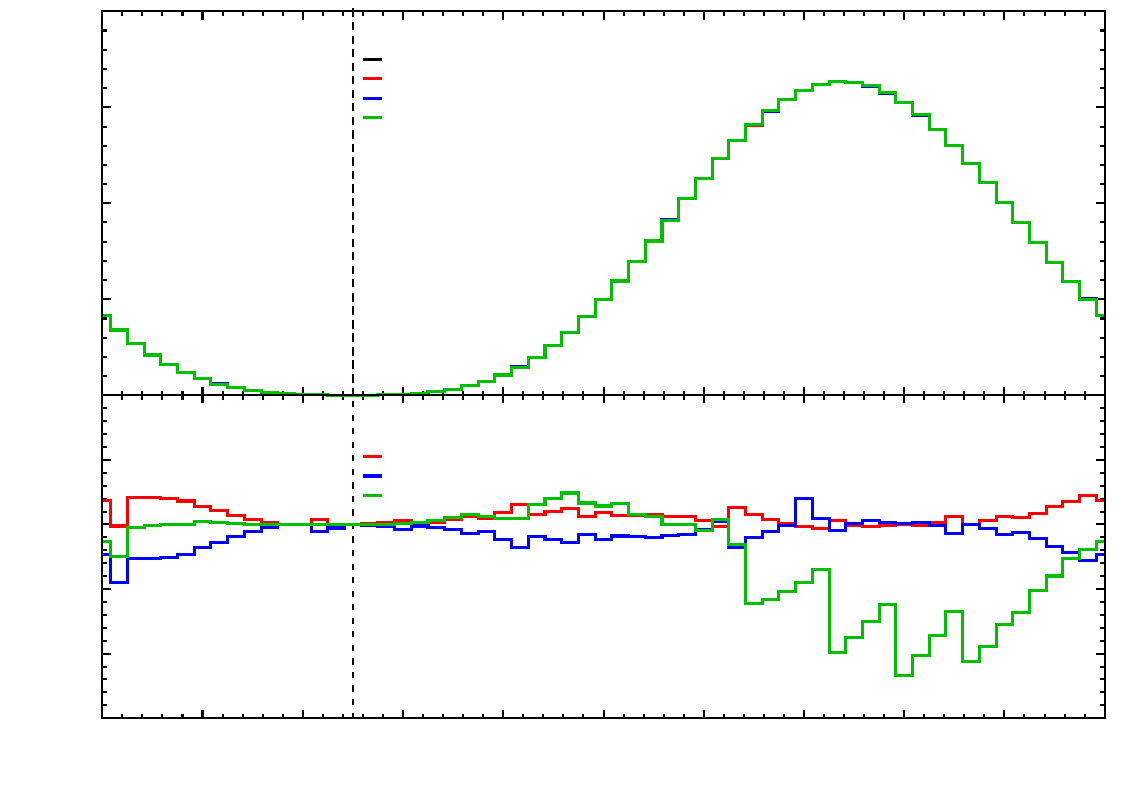
\includegraphics{pics/0_11a_11b_8_chi2_dCP}}%
    \gplfronttext
  \end{picture}%
\endgroup
}
	\resizebox{0.48\linewidth}{!}{% GNUPLOT: LaTeX picture with Postscript
\begingroup
  \makeatletter
  \providecommand\color[2][]{%
    \GenericError{(gnuplot) \space\space\space\@spaces}{%
      Package color not loaded in conjunction with
      terminal option `colourtext'%
    }{See the gnuplot documentation for explanation.%
    }{Either use 'blacktext' in gnuplot or load the package
      color.sty in LaTeX.}%
    \renewcommand\color[2][]{}%
  }%
  \providecommand\includegraphics[2][]{%
    \GenericError{(gnuplot) \space\space\space\@spaces}{%
      Package graphicx or graphics not loaded%
    }{See the gnuplot documentation for explanation.%
    }{The gnuplot epslatex terminal needs graphicx.sty or graphics.sty.}%
    \renewcommand\includegraphics[2][]{}%
  }%
  \providecommand\rotatebox[2]{#2}%
  \@ifundefined{ifGPcolor}{%
    \newif\ifGPcolor
    \GPcolortrue
  }{}%
  \@ifundefined{ifGPblacktext}{%
    \newif\ifGPblacktext
    \GPblacktexttrue
  }{}%
  % define a \g@addto@macro without @ in the name:
  \let\gplgaddtomacro\g@addto@macro
  % define empty templates for all commands taking text:
  \gdef\gplbacktext{}%
  \gdef\gplfronttext{}%
  \makeatother
  \ifGPblacktext
    % no textcolor at all
    \def\colorrgb#1{}%
    \def\colorgray#1{}%
  \else
    % gray or color?
    \ifGPcolor
      \def\colorrgb#1{\color[rgb]{#1}}%
      \def\colorgray#1{\color[gray]{#1}}%
      \expandafter\def\csname LTw\endcsname{\color{white}}%
      \expandafter\def\csname LTb\endcsname{\color{black}}%
      \expandafter\def\csname LTa\endcsname{\color{black}}%
      \expandafter\def\csname LT0\endcsname{\color[rgb]{1,0,0}}%
      \expandafter\def\csname LT1\endcsname{\color[rgb]{0,1,0}}%
      \expandafter\def\csname LT2\endcsname{\color[rgb]{0,0,1}}%
      \expandafter\def\csname LT3\endcsname{\color[rgb]{1,0,1}}%
      \expandafter\def\csname LT4\endcsname{\color[rgb]{0,1,1}}%
      \expandafter\def\csname LT5\endcsname{\color[rgb]{1,1,0}}%
      \expandafter\def\csname LT6\endcsname{\color[rgb]{0,0,0}}%
      \expandafter\def\csname LT7\endcsname{\color[rgb]{1,0.3,0}}%
      \expandafter\def\csname LT8\endcsname{\color[rgb]{0.5,0.5,0.5}}%
    \else
      % gray
      \def\colorrgb#1{\color{black}}%
      \def\colorgray#1{\color[gray]{#1}}%
      \expandafter\def\csname LTw\endcsname{\color{white}}%
      \expandafter\def\csname LTb\endcsname{\color{black}}%
      \expandafter\def\csname LTa\endcsname{\color{black}}%
      \expandafter\def\csname LT0\endcsname{\color{black}}%
      \expandafter\def\csname LT1\endcsname{\color{black}}%
      \expandafter\def\csname LT2\endcsname{\color{black}}%
      \expandafter\def\csname LT3\endcsname{\color{black}}%
      \expandafter\def\csname LT4\endcsname{\color{black}}%
      \expandafter\def\csname LT5\endcsname{\color{black}}%
      \expandafter\def\csname LT6\endcsname{\color{black}}%
      \expandafter\def\csname LT7\endcsname{\color{black}}%
      \expandafter\def\csname LT8\endcsname{\color{black}}%
    \fi
  \fi
    \setlength{\unitlength}{0.0500bp}%
    \ifx\gptboxheight\undefined%
      \newlength{\gptboxheight}%
      \newlength{\gptboxwidth}%
      \newsavebox{\gptboxtext}%
    \fi%
    \setlength{\fboxrule}{0.5pt}%
    \setlength{\fboxsep}{1pt}%
\begin{picture}(10800.00,7560.00)%
    \gplgaddtomacro\gplbacktext{%
      \csname LTb\endcsname%%
      \put(870,680){\makebox(0,0)[r]{\strut{}-0.6}}%
      \csname LTb\endcsname%%
      \put(870,1197){\makebox(0,0)[r]{\strut{}-0.4}}%
      \csname LTb\endcsname%%
      \put(870,1713){\makebox(0,0)[r]{\strut{}-0.2}}%
      \csname LTb\endcsname%%
      \put(870,2230){\makebox(0,0)[r]{\strut{}0}}%
      \csname LTb\endcsname%%
      \put(870,2747){\makebox(0,0)[r]{\strut{}0.2}}%
      \csname LTb\endcsname%%
      \put(870,3263){\makebox(0,0)[r]{\strut{}0.4}}%
      \csname LTb\endcsname%%
      \put(1614,494){\makebox(0,0){\strut{}2.47}}%
      \csname LTb\endcsname%%
      \put(2683,494){\makebox(0,0){\strut{}2.48}}%
      \csname LTb\endcsname%%
      \put(3752,494){\makebox(0,0){\strut{}2.49}}%
      \csname LTb\endcsname%%
      \put(4821,494){\makebox(0,0){\strut{}2.5}}%
      \csname LTb\endcsname%%
      \put(5890,494){\makebox(0,0){\strut{}2.51}}%
      \csname LTb\endcsname%%
      \put(6960,494){\makebox(0,0){\strut{}2.52}}%
      \csname LTb\endcsname%%
      \put(8029,494){\makebox(0,0){\strut{}2.53}}%
      \csname LTb\endcsname%%
      \put(9098,494){\makebox(0,0){\strut{}2.54}}%
      \csname LTb\endcsname%%
      \put(10167,494){\makebox(0,0){\strut{}2.55}}%
    }%
    \gplgaddtomacro\gplfronttext{%
      \csname LTb\endcsname%%
      \put(276,2230){\rotatebox{-270}{\makebox(0,0){\strut{}$\Delta \chi^2 - \Delta \chi^2_0$}}}%
      \csname LTb\endcsname%%
      \put(5783,215){\makebox(0,0){\strut{}$\Delta m_{32}^2 / 10^{-3}$}}%
      \csname LTb\endcsname%%
      \put(6345,2912){\makebox(0,0){\strut{}Difference}}%
      \csname LTb\endcsname%%
      \put(6164,2726){\makebox(0,0)[l]{\strut{}11a}}%
      \csname LTb\endcsname%%
      \put(6164,2540){\makebox(0,0)[l]{\strut{}11b}}%
      \csname LTb\endcsname%%
      \put(6164,2354){\makebox(0,0)[l]{\strut{}8}}%
    }%
    \gplgaddtomacro\gplbacktext{%
      \csname LTb\endcsname%%
      \put(870,3780){\makebox(0,0)[r]{\strut{}0}}%
      \csname LTb\endcsname%%
      \put(870,5623){\makebox(0,0)[r]{\strut{}10}}%
      \csname LTb\endcsname%%
      \put(870,7466){\makebox(0,0)[r]{\strut{}20}}%
      \csname LTb\endcsname%%
      \put(1614,3594){\makebox(0,0){\strut{}}}%
      \csname LTb\endcsname%%
      \put(2683,3594){\makebox(0,0){\strut{}}}%
      \csname LTb\endcsname%%
      \put(3752,3594){\makebox(0,0){\strut{}}}%
      \csname LTb\endcsname%%
      \put(4821,3594){\makebox(0,0){\strut{}}}%
      \csname LTb\endcsname%%
      \put(5890,3594){\makebox(0,0){\strut{}}}%
      \csname LTb\endcsname%%
      \put(6960,3594){\makebox(0,0){\strut{}}}%
      \csname LTb\endcsname%%
      \put(8029,3594){\makebox(0,0){\strut{}}}%
      \csname LTb\endcsname%%
      \put(9098,3594){\makebox(0,0){\strut{}}}%
      \csname LTb\endcsname%%
      \put(10167,3594){\makebox(0,0){\strut{}}}%
    }%
    \gplgaddtomacro\gplfronttext{%
      \csname LTb\endcsname%%
      \put(480,5623){\rotatebox{-270}{\makebox(0,0){\strut{}$\Delta \chi^2$}}}%
      \csname LTb\endcsname%%
      \put(5783,3538){\makebox(0,0){\strut{}}}%
      \csname LTb\endcsname%%
      \put(6127,7004){\makebox(0,0){\strut{}}}%
      \csname LTb\endcsname%%
      \put(6164,7004){\makebox(0,0)[l]{\strut{}0}}%
      \csname LTb\endcsname%%
      \put(6164,6818){\makebox(0,0)[l]{\strut{}11a}}%
      \csname LTb\endcsname%%
      \put(6164,6632){\makebox(0,0)[l]{\strut{}11b}}%
      \csname LTb\endcsname%%
      \put(6164,6446){\makebox(0,0)[l]{\strut{}8}}%
    }%
    \gplbacktext
    \put(0,0){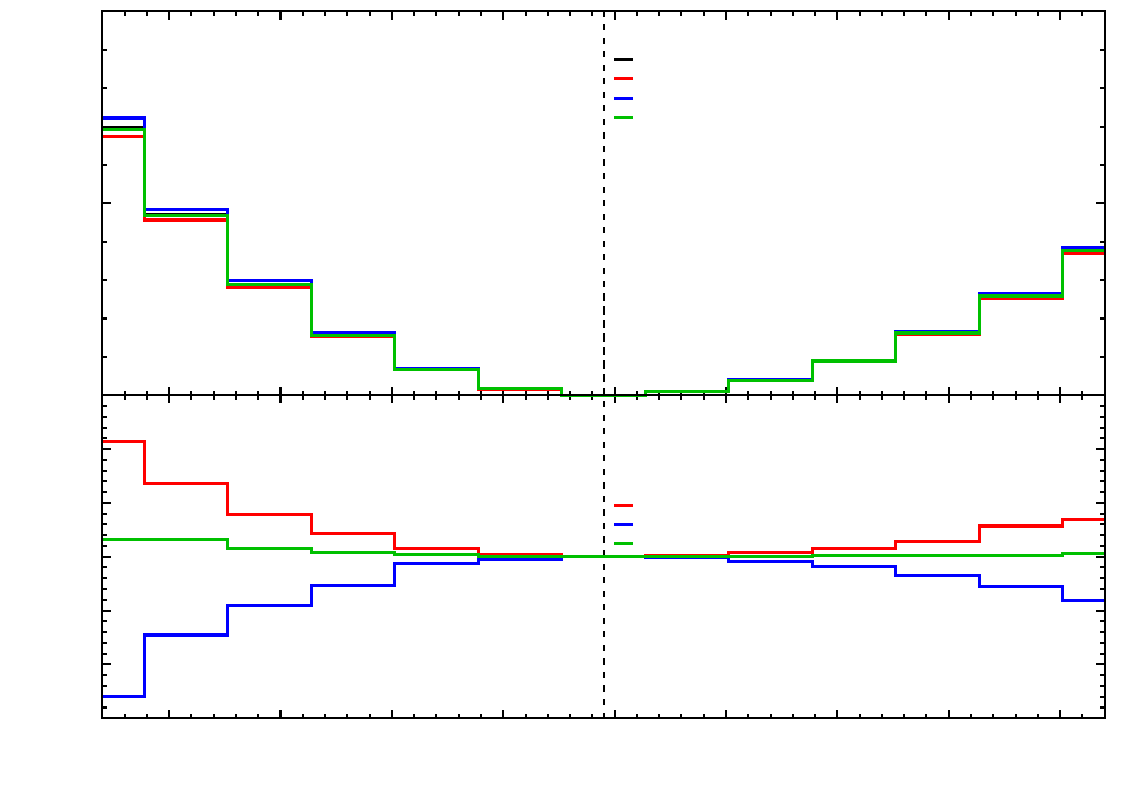
\includegraphics{pics/0_11a_11b_8_chi2_M23}}%
    \gplfronttext
  \end{picture}%
\endgroup
}
	\caption{$\chi^2$ profile for $\delta_\text{CP}$ (left) and $\Delta m_{32}^2$ (right). 
		The bottom panels show the difference of the different lines with the no systematic profile.}
	\label{fig:0_11a_11b_8_dCP_M23}
\end{figure}

\begin{figure}
	\centering
	\resizebox{0.48\linewidth}{!}{% GNUPLOT: LaTeX picture with Postscript
\begingroup
  \makeatletter
  \providecommand\color[2][]{%
    \GenericError{(gnuplot) \space\space\space\@spaces}{%
      Package color not loaded in conjunction with
      terminal option `colourtext'%
    }{See the gnuplot documentation for explanation.%
    }{Either use 'blacktext' in gnuplot or load the package
      color.sty in LaTeX.}%
    \renewcommand\color[2][]{}%
  }%
  \providecommand\includegraphics[2][]{%
    \GenericError{(gnuplot) \space\space\space\@spaces}{%
      Package graphicx or graphics not loaded%
    }{See the gnuplot documentation for explanation.%
    }{The gnuplot epslatex terminal needs graphicx.sty or graphics.sty.}%
    \renewcommand\includegraphics[2][]{}%
  }%
  \providecommand\rotatebox[2]{#2}%
  \@ifundefined{ifGPcolor}{%
    \newif\ifGPcolor
    \GPcolortrue
  }{}%
  \@ifundefined{ifGPblacktext}{%
    \newif\ifGPblacktext
    \GPblacktexttrue
  }{}%
  % define a \g@addto@macro without @ in the name:
  \let\gplgaddtomacro\g@addto@macro
  % define empty templates for all commands taking text:
  \gdef\gplbacktext{}%
  \gdef\gplfronttext{}%
  \makeatother
  \ifGPblacktext
    % no textcolor at all
    \def\colorrgb#1{}%
    \def\colorgray#1{}%
  \else
    % gray or color?
    \ifGPcolor
      \def\colorrgb#1{\color[rgb]{#1}}%
      \def\colorgray#1{\color[gray]{#1}}%
      \expandafter\def\csname LTw\endcsname{\color{white}}%
      \expandafter\def\csname LTb\endcsname{\color{black}}%
      \expandafter\def\csname LTa\endcsname{\color{black}}%
      \expandafter\def\csname LT0\endcsname{\color[rgb]{1,0,0}}%
      \expandafter\def\csname LT1\endcsname{\color[rgb]{0,1,0}}%
      \expandafter\def\csname LT2\endcsname{\color[rgb]{0,0,1}}%
      \expandafter\def\csname LT3\endcsname{\color[rgb]{1,0,1}}%
      \expandafter\def\csname LT4\endcsname{\color[rgb]{0,1,1}}%
      \expandafter\def\csname LT5\endcsname{\color[rgb]{1,1,0}}%
      \expandafter\def\csname LT6\endcsname{\color[rgb]{0,0,0}}%
      \expandafter\def\csname LT7\endcsname{\color[rgb]{1,0.3,0}}%
      \expandafter\def\csname LT8\endcsname{\color[rgb]{0.5,0.5,0.5}}%
    \else
      % gray
      \def\colorrgb#1{\color{black}}%
      \def\colorgray#1{\color[gray]{#1}}%
      \expandafter\def\csname LTw\endcsname{\color{white}}%
      \expandafter\def\csname LTb\endcsname{\color{black}}%
      \expandafter\def\csname LTa\endcsname{\color{black}}%
      \expandafter\def\csname LT0\endcsname{\color{black}}%
      \expandafter\def\csname LT1\endcsname{\color{black}}%
      \expandafter\def\csname LT2\endcsname{\color{black}}%
      \expandafter\def\csname LT3\endcsname{\color{black}}%
      \expandafter\def\csname LT4\endcsname{\color{black}}%
      \expandafter\def\csname LT5\endcsname{\color{black}}%
      \expandafter\def\csname LT6\endcsname{\color{black}}%
      \expandafter\def\csname LT7\endcsname{\color{black}}%
      \expandafter\def\csname LT8\endcsname{\color{black}}%
    \fi
  \fi
    \setlength{\unitlength}{0.0500bp}%
    \ifx\gptboxheight\undefined%
      \newlength{\gptboxheight}%
      \newlength{\gptboxwidth}%
      \newsavebox{\gptboxtext}%
    \fi%
    \setlength{\fboxrule}{0.5pt}%
    \setlength{\fboxsep}{1pt}%
\begin{picture}(10800.00,7560.00)%
    \gplgaddtomacro\gplbacktext{%
      \csname LTb\endcsname%%
      \put(870,680){\makebox(0,0)[r]{\strut{}-0.01}}%
      \csname LTb\endcsname%%
      \put(870,1123){\makebox(0,0)[r]{\strut{}0}}%
      \csname LTb\endcsname%%
      \put(870,1566){\makebox(0,0)[r]{\strut{}0.01}}%
      \csname LTb\endcsname%%
      \put(870,2009){\makebox(0,0)[r]{\strut{}0.02}}%
      \csname LTb\endcsname%%
      \put(870,2451){\makebox(0,0)[r]{\strut{}0.03}}%
      \csname LTb\endcsname%%
      \put(870,2894){\makebox(0,0)[r]{\strut{}0.04}}%
      \csname LTb\endcsname%%
      \put(870,3337){\makebox(0,0)[r]{\strut{}0.05}}%
      \csname LTb\endcsname%%
      \put(972,494){\makebox(0,0){\strut{}0.07}}%
      \csname LTb\endcsname%%
      \put(2576,494){\makebox(0,0){\strut{}0.075}}%
      \csname LTb\endcsname%%
      \put(4180,494){\makebox(0,0){\strut{}0.08}}%
      \csname LTb\endcsname%%
      \put(5784,494){\makebox(0,0){\strut{}0.085}}%
      \csname LTb\endcsname%%
      \put(7387,494){\makebox(0,0){\strut{}0.09}}%
      \csname LTb\endcsname%%
      \put(8991,494){\makebox(0,0){\strut{}0.095}}%
      \csname LTb\endcsname%%
      \put(10595,494){\makebox(0,0){\strut{}0.1}}%
    }%
    \gplgaddtomacro\gplfronttext{%
      \csname LTb\endcsname%%
      \put(174,2230){\rotatebox{-270}{\makebox(0,0){\strut{}$\Delta \chi^2 - \Delta \chi^2_0$}}}%
      \csname LTb\endcsname%%
      \put(5783,215){\makebox(0,0){\strut{}$\sin^2 2 \theta_{13}$}}%
      \csname LTb\endcsname%%
      \put(6364,2358){\makebox(0,0){\strut{}Difference}}%
      \csname LTb\endcsname%%
      \put(6183,2172){\makebox(0,0)[l]{\strut{}11a}}%
      \csname LTb\endcsname%%
      \put(6183,1986){\makebox(0,0)[l]{\strut{}11b}}%
      \csname LTb\endcsname%%
      \put(6183,1800){\makebox(0,0)[l]{\strut{}8}}%
    }%
    \gplgaddtomacro\gplbacktext{%
      \csname LTb\endcsname%%
      \put(870,3780){\makebox(0,0)[r]{\strut{}0}}%
      \csname LTb\endcsname%%
      \put(870,5145){\makebox(0,0)[r]{\strut{}10}}%
      \csname LTb\endcsname%%
      \put(870,6510){\makebox(0,0)[r]{\strut{}20}}%
      \csname LTb\endcsname%%
      \put(972,3594){\makebox(0,0){\strut{}}}%
      \csname LTb\endcsname%%
      \put(2576,3594){\makebox(0,0){\strut{}}}%
      \csname LTb\endcsname%%
      \put(4180,3594){\makebox(0,0){\strut{}}}%
      \csname LTb\endcsname%%
      \put(5784,3594){\makebox(0,0){\strut{}}}%
      \csname LTb\endcsname%%
      \put(7387,3594){\makebox(0,0){\strut{}}}%
      \csname LTb\endcsname%%
      \put(8991,3594){\makebox(0,0){\strut{}}}%
      \csname LTb\endcsname%%
      \put(10595,3594){\makebox(0,0){\strut{}}}%
    }%
    \gplgaddtomacro\gplfronttext{%
      \csname LTb\endcsname%%
      \put(480,5623){\rotatebox{-270}{\makebox(0,0){\strut{}$\Delta \chi^2$}}}%
      \csname LTb\endcsname%%
      \put(5783,3538){\makebox(0,0){\strut{}}}%
      \csname LTb\endcsname%%
      \put(6146,7004){\makebox(0,0){\strut{}}}%
      \csname LTb\endcsname%%
      \put(6183,7004){\makebox(0,0)[l]{\strut{}0}}%
      \csname LTb\endcsname%%
      \put(6183,6818){\makebox(0,0)[l]{\strut{}11a}}%
      \csname LTb\endcsname%%
      \put(6183,6632){\makebox(0,0)[l]{\strut{}11b}}%
      \csname LTb\endcsname%%
      \put(6183,6446){\makebox(0,0)[l]{\strut{}8}}%
    }%
    \gplbacktext
    \put(0,0){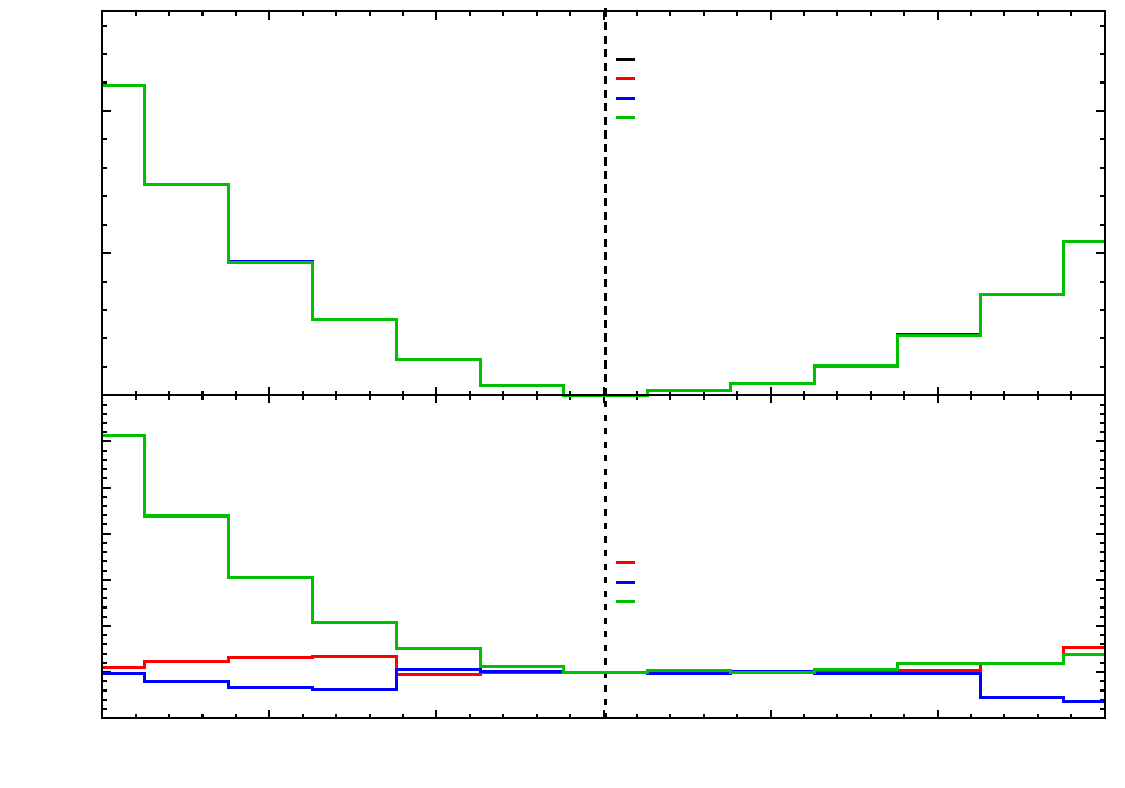
\includegraphics{pics/0_11a_11b_8_chi2_S13}}%
    \gplfronttext
  \end{picture}%
\endgroup
}
	\resizebox{0.48\linewidth}{!}{% GNUPLOT: LaTeX picture with Postscript
\begingroup
  \makeatletter
  \providecommand\color[2][]{%
    \GenericError{(gnuplot) \space\space\space\@spaces}{%
      Package color not loaded in conjunction with
      terminal option `colourtext'%
    }{See the gnuplot documentation for explanation.%
    }{Either use 'blacktext' in gnuplot or load the package
      color.sty in LaTeX.}%
    \renewcommand\color[2][]{}%
  }%
  \providecommand\includegraphics[2][]{%
    \GenericError{(gnuplot) \space\space\space\@spaces}{%
      Package graphicx or graphics not loaded%
    }{See the gnuplot documentation for explanation.%
    }{The gnuplot epslatex terminal needs graphicx.sty or graphics.sty.}%
    \renewcommand\includegraphics[2][]{}%
  }%
  \providecommand\rotatebox[2]{#2}%
  \@ifundefined{ifGPcolor}{%
    \newif\ifGPcolor
    \GPcolortrue
  }{}%
  \@ifundefined{ifGPblacktext}{%
    \newif\ifGPblacktext
    \GPblacktexttrue
  }{}%
  % define a \g@addto@macro without @ in the name:
  \let\gplgaddtomacro\g@addto@macro
  % define empty templates for all commands taking text:
  \gdef\gplbacktext{}%
  \gdef\gplfronttext{}%
  \makeatother
  \ifGPblacktext
    % no textcolor at all
    \def\colorrgb#1{}%
    \def\colorgray#1{}%
  \else
    % gray or color?
    \ifGPcolor
      \def\colorrgb#1{\color[rgb]{#1}}%
      \def\colorgray#1{\color[gray]{#1}}%
      \expandafter\def\csname LTw\endcsname{\color{white}}%
      \expandafter\def\csname LTb\endcsname{\color{black}}%
      \expandafter\def\csname LTa\endcsname{\color{black}}%
      \expandafter\def\csname LT0\endcsname{\color[rgb]{1,0,0}}%
      \expandafter\def\csname LT1\endcsname{\color[rgb]{0,1,0}}%
      \expandafter\def\csname LT2\endcsname{\color[rgb]{0,0,1}}%
      \expandafter\def\csname LT3\endcsname{\color[rgb]{1,0,1}}%
      \expandafter\def\csname LT4\endcsname{\color[rgb]{0,1,1}}%
      \expandafter\def\csname LT5\endcsname{\color[rgb]{1,1,0}}%
      \expandafter\def\csname LT6\endcsname{\color[rgb]{0,0,0}}%
      \expandafter\def\csname LT7\endcsname{\color[rgb]{1,0.3,0}}%
      \expandafter\def\csname LT8\endcsname{\color[rgb]{0.5,0.5,0.5}}%
    \else
      % gray
      \def\colorrgb#1{\color{black}}%
      \def\colorgray#1{\color[gray]{#1}}%
      \expandafter\def\csname LTw\endcsname{\color{white}}%
      \expandafter\def\csname LTb\endcsname{\color{black}}%
      \expandafter\def\csname LTa\endcsname{\color{black}}%
      \expandafter\def\csname LT0\endcsname{\color{black}}%
      \expandafter\def\csname LT1\endcsname{\color{black}}%
      \expandafter\def\csname LT2\endcsname{\color{black}}%
      \expandafter\def\csname LT3\endcsname{\color{black}}%
      \expandafter\def\csname LT4\endcsname{\color{black}}%
      \expandafter\def\csname LT5\endcsname{\color{black}}%
      \expandafter\def\csname LT6\endcsname{\color{black}}%
      \expandafter\def\csname LT7\endcsname{\color{black}}%
      \expandafter\def\csname LT8\endcsname{\color{black}}%
    \fi
  \fi
    \setlength{\unitlength}{0.0500bp}%
    \ifx\gptboxheight\undefined%
      \newlength{\gptboxheight}%
      \newlength{\gptboxwidth}%
      \newsavebox{\gptboxtext}%
    \fi%
    \setlength{\fboxrule}{0.5pt}%
    \setlength{\fboxsep}{1pt}%
\begin{picture}(10800.00,7560.00)%
    \gplgaddtomacro\gplbacktext{%
      \csname LTb\endcsname%%
      \put(870,680){\makebox(0,0)[r]{\strut{}-0.3}}%
      \csname LTb\endcsname%%
      \put(870,1197){\makebox(0,0)[r]{\strut{}-0.2}}%
      \csname LTb\endcsname%%
      \put(870,1713){\makebox(0,0)[r]{\strut{}-0.1}}%
      \csname LTb\endcsname%%
      \put(870,2230){\makebox(0,0)[r]{\strut{}0}}%
      \csname LTb\endcsname%%
      \put(870,2747){\makebox(0,0)[r]{\strut{}0.1}}%
      \csname LTb\endcsname%%
      \put(870,3263){\makebox(0,0)[r]{\strut{}0.2}}%
      \csname LTb\endcsname%%
      \put(1853,494){\makebox(0,0){\strut{}0.44}}%
      \csname LTb\endcsname%%
      \put(3110,494){\makebox(0,0){\strut{}0.46}}%
      \csname LTb\endcsname%%
      \put(4368,494){\makebox(0,0){\strut{}0.48}}%
      \csname LTb\endcsname%%
      \put(5626,494){\makebox(0,0){\strut{}0.5}}%
      \csname LTb\endcsname%%
      \put(6884,494){\makebox(0,0){\strut{}0.52}}%
      \csname LTb\endcsname%%
      \put(8142,494){\makebox(0,0){\strut{}0.54}}%
      \csname LTb\endcsname%%
      \put(9400,494){\makebox(0,0){\strut{}0.56}}%
    }%
    \gplgaddtomacro\gplfronttext{%
      \csname LTb\endcsname%%
      \put(276,2230){\rotatebox{-270}{\makebox(0,0){\strut{}$\Delta \chi^2 - \Delta \chi^2_0$}}}%
      \csname LTb\endcsname%%
      \put(5783,215){\makebox(0,0){\strut{}$\sin^2 \theta_{23}$}}%
      \csname LTb\endcsname%%
      \put(7948,2912){\makebox(0,0){\strut{}Difference}}%
      \csname LTb\endcsname%%
      \put(7767,2726){\makebox(0,0)[l]{\strut{}11a}}%
      \csname LTb\endcsname%%
      \put(7767,2540){\makebox(0,0)[l]{\strut{}11b}}%
      \csname LTb\endcsname%%
      \put(7767,2354){\makebox(0,0)[l]{\strut{}8}}%
    }%
    \gplgaddtomacro\gplbacktext{%
      \csname LTb\endcsname%%
      \put(870,3780){\makebox(0,0)[r]{\strut{}0}}%
      \csname LTb\endcsname%%
      \put(870,4458){\makebox(0,0)[r]{\strut{}25}}%
      \csname LTb\endcsname%%
      \put(870,5135){\makebox(0,0)[r]{\strut{}50}}%
      \csname LTb\endcsname%%
      \put(870,5813){\makebox(0,0)[r]{\strut{}75}}%
      \csname LTb\endcsname%%
      \put(870,6490){\makebox(0,0)[r]{\strut{}100}}%
      \csname LTb\endcsname%%
      \put(870,7168){\makebox(0,0)[r]{\strut{}125}}%
      \csname LTb\endcsname%%
      \put(1853,3594){\makebox(0,0){\strut{}}}%
      \csname LTb\endcsname%%
      \put(3110,3594){\makebox(0,0){\strut{}}}%
      \csname LTb\endcsname%%
      \put(4368,3594){\makebox(0,0){\strut{}}}%
      \csname LTb\endcsname%%
      \put(5626,3594){\makebox(0,0){\strut{}}}%
      \csname LTb\endcsname%%
      \put(6884,3594){\makebox(0,0){\strut{}}}%
      \csname LTb\endcsname%%
      \put(8142,3594){\makebox(0,0){\strut{}}}%
      \csname LTb\endcsname%%
      \put(9400,3594){\makebox(0,0){\strut{}}}%
    }%
    \gplgaddtomacro\gplfronttext{%
      \csname LTb\endcsname%%
      \put(378,5623){\rotatebox{-270}{\makebox(0,0){\strut{}$\Delta \chi^2$}}}%
      \csname LTb\endcsname%%
      \put(5783,3538){\makebox(0,0){\strut{}}}%
      \csname LTb\endcsname%%
      \put(7730,7004){\makebox(0,0){\strut{}}}%
      \csname LTb\endcsname%%
      \put(7767,7004){\makebox(0,0)[l]{\strut{}0}}%
      \csname LTb\endcsname%%
      \put(7767,6818){\makebox(0,0)[l]{\strut{}11a}}%
      \csname LTb\endcsname%%
      \put(7767,6632){\makebox(0,0)[l]{\strut{}11b}}%
      \csname LTb\endcsname%%
      \put(7767,6446){\makebox(0,0)[l]{\strut{}8}}%
    }%
    \gplbacktext
    \put(0,0){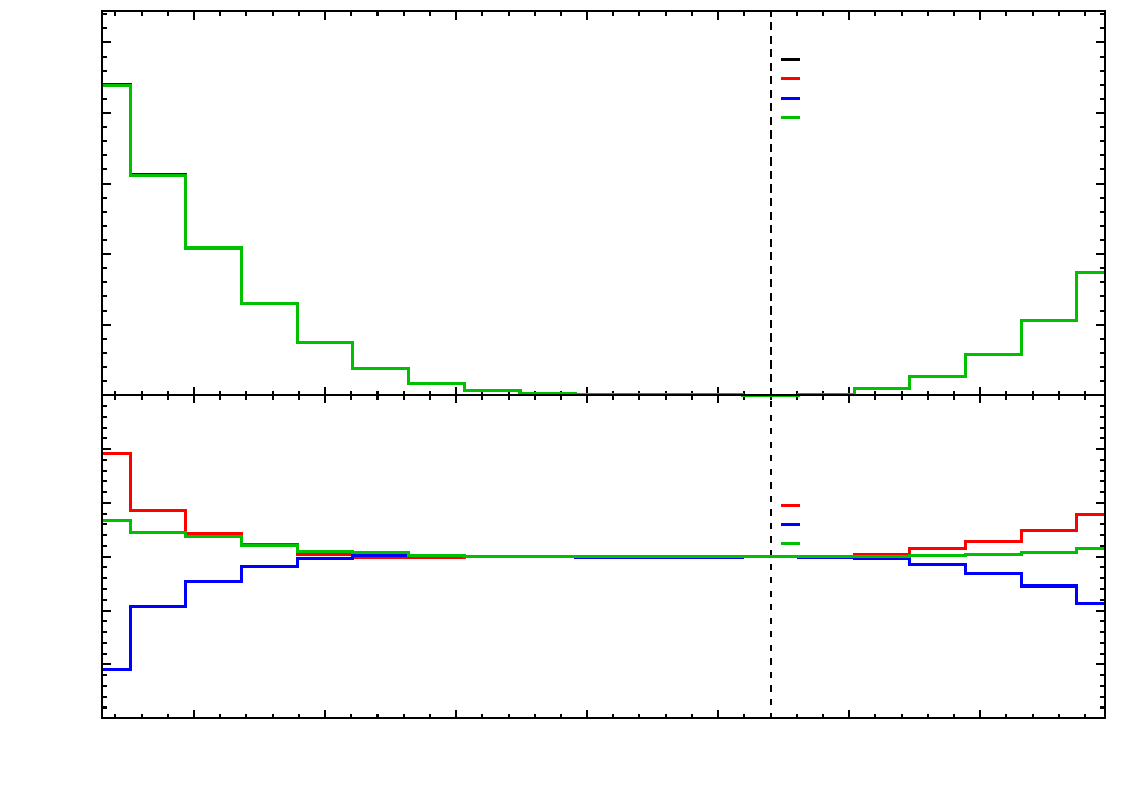
\includegraphics{pics/0_11a_11b_8_chi2_S23}}%
    \gplfronttext
  \end{picture}%
\endgroup
}
	\caption{$\chi^2$ profile for $\sin^2 2\theta_{13}$ (left) and $sin^2 \theta_{23}$ (right). 
		The bottom panels show the difference of the different lines with the no systematic profile.}
	\label{fig:0_11a_11b_8_S13_S23}
\end{figure}

\begin{figure}
	\centering
	\resizebox{0.48\linewidth}{!}{% GNUPLOT: LaTeX picture with Postscript
\begingroup
  \makeatletter
  \providecommand\color[2][]{%
    \GenericError{(gnuplot) \space\space\space\@spaces}{%
      Package color not loaded in conjunction with
      terminal option `colourtext'%
    }{See the gnuplot documentation for explanation.%
    }{Either use 'blacktext' in gnuplot or load the package
      color.sty in LaTeX.}%
    \renewcommand\color[2][]{}%
  }%
  \providecommand\includegraphics[2][]{%
    \GenericError{(gnuplot) \space\space\space\@spaces}{%
      Package graphicx or graphics not loaded%
    }{See the gnuplot documentation for explanation.%
    }{The gnuplot epslatex terminal needs graphicx.sty or graphics.sty.}%
    \renewcommand\includegraphics[2][]{}%
  }%
  \providecommand\rotatebox[2]{#2}%
  \@ifundefined{ifGPcolor}{%
    \newif\ifGPcolor
    \GPcolortrue
  }{}%
  \@ifundefined{ifGPblacktext}{%
    \newif\ifGPblacktext
    \GPblacktexttrue
  }{}%
  % define a \g@addto@macro without @ in the name:
  \let\gplgaddtomacro\g@addto@macro
  % define empty templates for all commands taking text:
  \gdef\gplbacktext{}%
  \gdef\gplfronttext{}%
  \makeatother
  \ifGPblacktext
    % no textcolor at all
    \def\colorrgb#1{}%
    \def\colorgray#1{}%
  \else
    % gray or color?
    \ifGPcolor
      \def\colorrgb#1{\color[rgb]{#1}}%
      \def\colorgray#1{\color[gray]{#1}}%
      \expandafter\def\csname LTw\endcsname{\color{white}}%
      \expandafter\def\csname LTb\endcsname{\color{black}}%
      \expandafter\def\csname LTa\endcsname{\color{black}}%
      \expandafter\def\csname LT0\endcsname{\color[rgb]{1,0,0}}%
      \expandafter\def\csname LT1\endcsname{\color[rgb]{0,1,0}}%
      \expandafter\def\csname LT2\endcsname{\color[rgb]{0,0,1}}%
      \expandafter\def\csname LT3\endcsname{\color[rgb]{1,0,1}}%
      \expandafter\def\csname LT4\endcsname{\color[rgb]{0,1,1}}%
      \expandafter\def\csname LT5\endcsname{\color[rgb]{1,1,0}}%
      \expandafter\def\csname LT6\endcsname{\color[rgb]{0,0,0}}%
      \expandafter\def\csname LT7\endcsname{\color[rgb]{1,0.3,0}}%
      \expandafter\def\csname LT8\endcsname{\color[rgb]{0.5,0.5,0.5}}%
    \else
      % gray
      \def\colorrgb#1{\color{black}}%
      \def\colorgray#1{\color[gray]{#1}}%
      \expandafter\def\csname LTw\endcsname{\color{white}}%
      \expandafter\def\csname LTb\endcsname{\color{black}}%
      \expandafter\def\csname LTa\endcsname{\color{black}}%
      \expandafter\def\csname LT0\endcsname{\color{black}}%
      \expandafter\def\csname LT1\endcsname{\color{black}}%
      \expandafter\def\csname LT2\endcsname{\color{black}}%
      \expandafter\def\csname LT3\endcsname{\color{black}}%
      \expandafter\def\csname LT4\endcsname{\color{black}}%
      \expandafter\def\csname LT5\endcsname{\color{black}}%
      \expandafter\def\csname LT6\endcsname{\color{black}}%
      \expandafter\def\csname LT7\endcsname{\color{black}}%
      \expandafter\def\csname LT8\endcsname{\color{black}}%
    \fi
  \fi
    \setlength{\unitlength}{0.0500bp}%
    \ifx\gptboxheight\undefined%
      \newlength{\gptboxheight}%
      \newlength{\gptboxwidth}%
      \newsavebox{\gptboxtext}%
    \fi%
    \setlength{\fboxrule}{0.5pt}%
    \setlength{\fboxsep}{1pt}%
\begin{picture}(10800.00,7560.00)%
    \gplgaddtomacro\gplbacktext{%
      \csname LTb\endcsname%%
      \put(747,1047){\makebox(0,0)[r]{\strut{}2.47}}%
      \csname LTb\endcsname%%
      \put(747,1800){\makebox(0,0)[r]{\strut{}2.48}}%
      \csname LTb\endcsname%%
      \put(747,2553){\makebox(0,0)[r]{\strut{}2.49}}%
      \csname LTb\endcsname%%
      \put(747,3306){\makebox(0,0)[r]{\strut{}2.5}}%
      \csname LTb\endcsname%%
      \put(747,4059){\makebox(0,0)[r]{\strut{}2.51}}%
      \csname LTb\endcsname%%
      \put(747,4812){\makebox(0,0)[r]{\strut{}2.52}}%
      \csname LTb\endcsname%%
      \put(747,5566){\makebox(0,0)[r]{\strut{}2.53}}%
      \csname LTb\endcsname%%
      \put(747,6319){\makebox(0,0)[r]{\strut{}2.54}}%
      \csname LTb\endcsname%%
      \put(747,7072){\makebox(0,0)[r]{\strut{}2.55}}%
      \csname LTb\endcsname%%
      \put(1731,409){\makebox(0,0){\strut{}0.44}}%
      \csname LTb\endcsname%%
      \put(2992,409){\makebox(0,0){\strut{}0.46}}%
      \csname LTb\endcsname%%
      \put(4253,409){\makebox(0,0){\strut{}0.48}}%
      \csname LTb\endcsname%%
      \put(5513,409){\makebox(0,0){\strut{}0.5}}%
      \csname LTb\endcsname%%
      \put(6774,409){\makebox(0,0){\strut{}0.52}}%
      \csname LTb\endcsname%%
      \put(8035,409){\makebox(0,0){\strut{}0.54}}%
      \csname LTb\endcsname%%
      \put(9295,409){\makebox(0,0){\strut{}0.56}}%
      \csname LTb\endcsname%%
      \put(7315,4021){\makebox(0,0)[l]{\strut{}}}%
    }%
    \gplgaddtomacro\gplfronttext{%
      \csname LTb\endcsname%%
      \put(153,3984){\rotatebox{-270}{\makebox(0,0){\strut{}$\Delta m_{32}^2 / 10^{-3}$}}}%
      \csname LTb\endcsname%%
      \put(5671,130){\makebox(0,0){\strut{}$\sin^2 \theta_{23}$}}%
      \csname LTb\endcsname%%
      \put(9705,7206){\makebox(0,0)[r]{\strut{}0}}%
      \csname LTb\endcsname%%
      \put(9705,7020){\makebox(0,0)[r]{\strut{}11a}}%
      \csname LTb\endcsname%%
      \put(9705,6834){\makebox(0,0)[r]{\strut{}11b}}%
      \csname LTb\endcsname%%
      \put(9705,6648){\makebox(0,0)[r]{\strut{}8}}%
    }%
    \gplbacktext
    \put(0,0){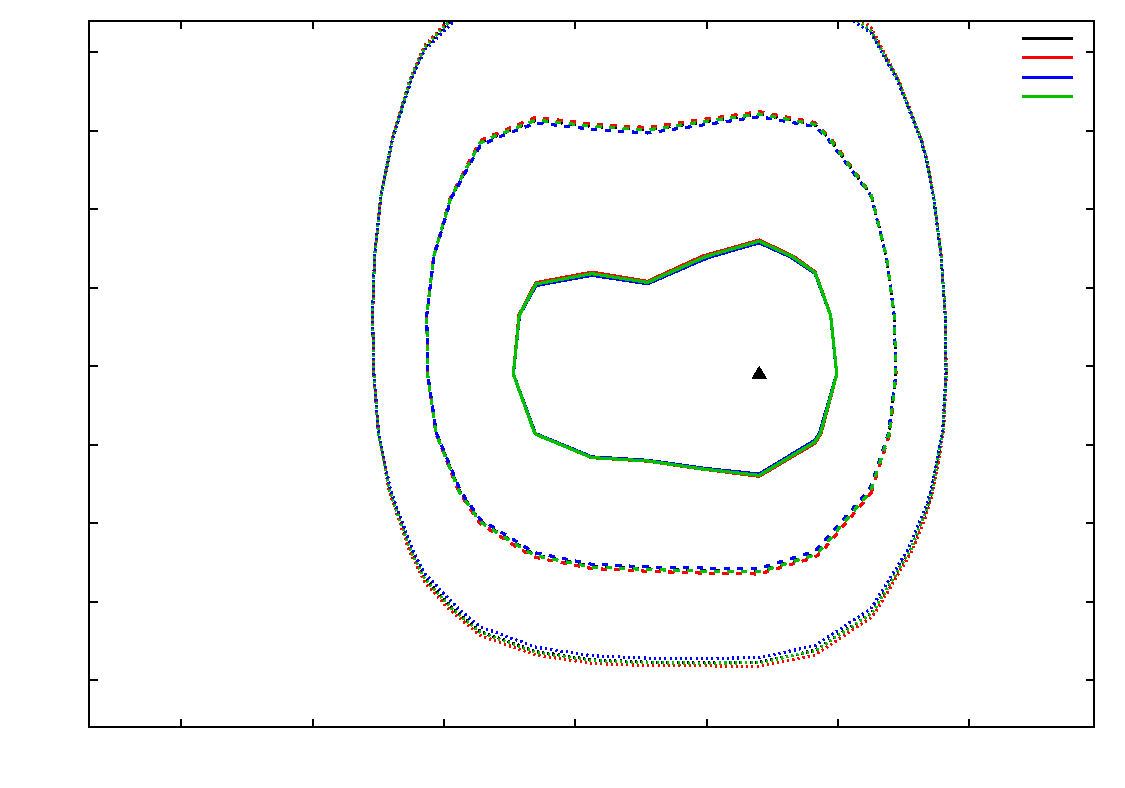
\includegraphics{pics/0_11a_11b_8_cont_S23_M23}}%
    \gplfronttext
  \end{picture}%
\endgroup
}	%%%%%%%%%%%this is important
	\caption{Contour plot of the $\chi^2$ profile for $\Delta m_{23}^2$ vs.\  $sin^2 \theta_{23}$ %
		for correlated (left) and anticorrelated (right) systematics. 
		The inner contour and outer contour corresponds respectively to the $1\sigma$ and $3\sigma$ %
		contour lines.}
	\label{fig:0_11a_11b_8_S23_M23}
\end{figure}

\begin{figure}
	\centering
	\resizebox{0.48\linewidth}{!}{% GNUPLOT: LaTeX picture with Postscript
\begingroup
  \makeatletter
  \providecommand\color[2][]{%
    \GenericError{(gnuplot) \space\space\space\@spaces}{%
      Package color not loaded in conjunction with
      terminal option `colourtext'%
    }{See the gnuplot documentation for explanation.%
    }{Either use 'blacktext' in gnuplot or load the package
      color.sty in LaTeX.}%
    \renewcommand\color[2][]{}%
  }%
  \providecommand\includegraphics[2][]{%
    \GenericError{(gnuplot) \space\space\space\@spaces}{%
      Package graphicx or graphics not loaded%
    }{See the gnuplot documentation for explanation.%
    }{The gnuplot epslatex terminal needs graphicx.sty or graphics.sty.}%
    \renewcommand\includegraphics[2][]{}%
  }%
  \providecommand\rotatebox[2]{#2}%
  \@ifundefined{ifGPcolor}{%
    \newif\ifGPcolor
    \GPcolortrue
  }{}%
  \@ifundefined{ifGPblacktext}{%
    \newif\ifGPblacktext
    \GPblacktexttrue
  }{}%
  % define a \g@addto@macro without @ in the name:
  \let\gplgaddtomacro\g@addto@macro
  % define empty templates for all commands taking text:
  \gdef\gplbacktext{}%
  \gdef\gplfronttext{}%
  \makeatother
  \ifGPblacktext
    % no textcolor at all
    \def\colorrgb#1{}%
    \def\colorgray#1{}%
  \else
    % gray or color?
    \ifGPcolor
      \def\colorrgb#1{\color[rgb]{#1}}%
      \def\colorgray#1{\color[gray]{#1}}%
      \expandafter\def\csname LTw\endcsname{\color{white}}%
      \expandafter\def\csname LTb\endcsname{\color{black}}%
      \expandafter\def\csname LTa\endcsname{\color{black}}%
      \expandafter\def\csname LT0\endcsname{\color[rgb]{1,0,0}}%
      \expandafter\def\csname LT1\endcsname{\color[rgb]{0,1,0}}%
      \expandafter\def\csname LT2\endcsname{\color[rgb]{0,0,1}}%
      \expandafter\def\csname LT3\endcsname{\color[rgb]{1,0,1}}%
      \expandafter\def\csname LT4\endcsname{\color[rgb]{0,1,1}}%
      \expandafter\def\csname LT5\endcsname{\color[rgb]{1,1,0}}%
      \expandafter\def\csname LT6\endcsname{\color[rgb]{0,0,0}}%
      \expandafter\def\csname LT7\endcsname{\color[rgb]{1,0.3,0}}%
      \expandafter\def\csname LT8\endcsname{\color[rgb]{0.5,0.5,0.5}}%
    \else
      % gray
      \def\colorrgb#1{\color{black}}%
      \def\colorgray#1{\color[gray]{#1}}%
      \expandafter\def\csname LTw\endcsname{\color{white}}%
      \expandafter\def\csname LTb\endcsname{\color{black}}%
      \expandafter\def\csname LTa\endcsname{\color{black}}%
      \expandafter\def\csname LT0\endcsname{\color{black}}%
      \expandafter\def\csname LT1\endcsname{\color{black}}%
      \expandafter\def\csname LT2\endcsname{\color{black}}%
      \expandafter\def\csname LT3\endcsname{\color{black}}%
      \expandafter\def\csname LT4\endcsname{\color{black}}%
      \expandafter\def\csname LT5\endcsname{\color{black}}%
      \expandafter\def\csname LT6\endcsname{\color{black}}%
      \expandafter\def\csname LT7\endcsname{\color{black}}%
      \expandafter\def\csname LT8\endcsname{\color{black}}%
    \fi
  \fi
    \setlength{\unitlength}{0.0500bp}%
    \ifx\gptboxheight\undefined%
      \newlength{\gptboxheight}%
      \newlength{\gptboxwidth}%
      \newsavebox{\gptboxtext}%
    \fi%
    \setlength{\fboxrule}{0.5pt}%
    \setlength{\fboxsep}{1pt}%
\begin{picture}(11520.00,6480.00)%
    \gplgaddtomacro\gplbacktext{%
      \csname LTb\endcsname%%
      \put(550,704){\makebox(0,0)[r]{\strut{}0}}%
      \put(550,2093){\makebox(0,0)[r]{\strut{}2}}%
      \put(550,3482){\makebox(0,0)[r]{\strut{}4}}%
      \put(550,4870){\makebox(0,0)[r]{\strut{}6}}%
      \put(550,6259){\makebox(0,0)[r]{\strut{}8}}%
      \put(917,484){\makebox(0,0){\strut{}-1.0$\pi$}}%
      \put(2579,484){\makebox(0,0){\strut{}-0.6$\pi$}}%
      \put(4241,484){\makebox(0,0){\strut{}-0.3$\pi$}}%
      \put(5903,484){\makebox(0,0){\strut{}0.0$\pi$}}%
      \put(7564,484){\makebox(0,0){\strut{}0.3$\pi$}}%
      \put(9226,484){\makebox(0,0){\strut{}0.6$\pi$}}%
      \put(10888,484){\makebox(0,0){\strut{}1.0$\pi$}}%
      \put(5903,4523){\makebox(0,0){\strut{}$5 \sigma$}}%
      \put(5903,3134){\makebox(0,0){\strut{}$3 \sigma$}}%
    }%
    \gplgaddtomacro\gplfronttext{%
      \csname LTb\endcsname%%
      \put(198,3481){\rotatebox{-270}{\makebox(0,0){\strut{}$\sigma (\delta_\text{CP})$}}}%
      \put(5902,154){\makebox(0,0){\strut{}$\delta_\text{CP}$}}%
      \csname LTb\endcsname%%
      \put(1339,6086){\makebox(0,0)[l]{\strut{}0}}%
      \csname LTb\endcsname%%
      \put(1339,5866){\makebox(0,0)[l]{\strut{}11a}}%
      \csname LTb\endcsname%%
      \put(1339,5646){\makebox(0,0)[l]{\strut{}11b}}%
      \csname LTb\endcsname%%
      \put(1339,5426){\makebox(0,0)[l]{\strut{}8}}%
    }%
    \gplbacktext
    \put(0,0){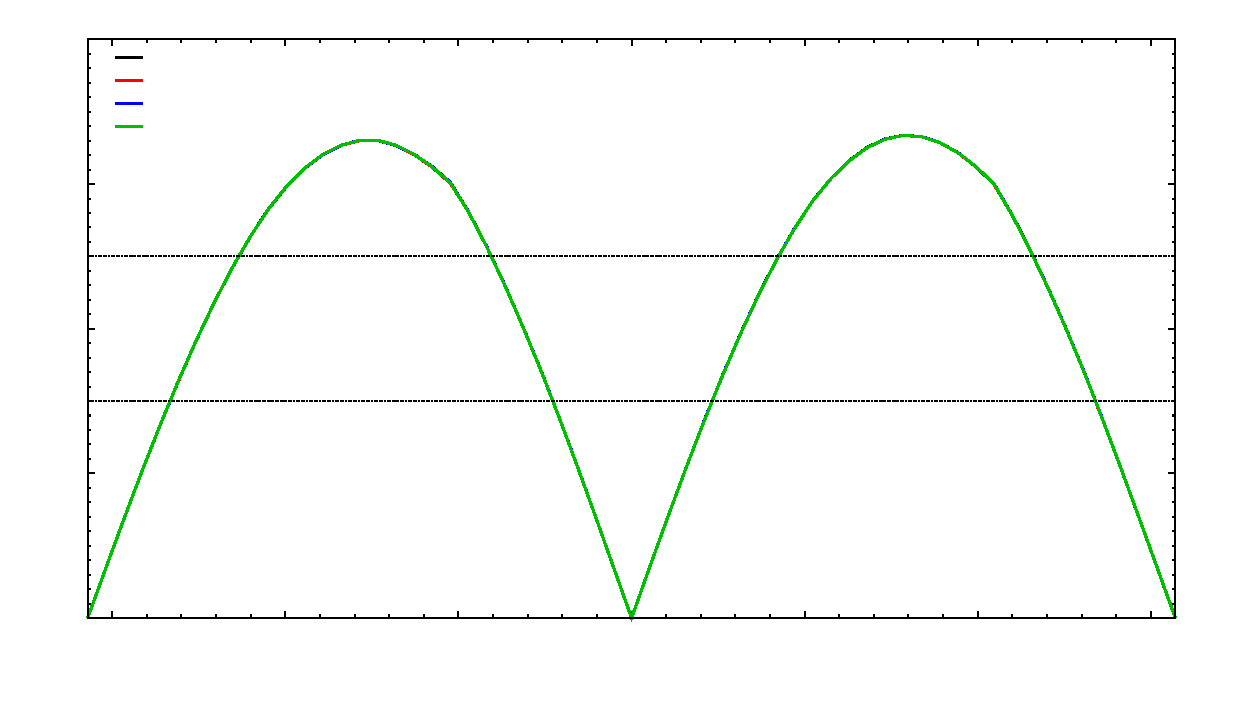
\includegraphics{pics/0_11a_11b_8_sensitivity}}%
    \gplfronttext
  \end{picture}%
\endgroup
}
	\resizebox{0.48\linewidth}{!}{% GNUPLOT: LaTeX picture with Postscript
\begingroup
  \makeatletter
  \providecommand\color[2][]{%
    \GenericError{(gnuplot) \space\space\space\@spaces}{%
      Package color not loaded in conjunction with
      terminal option `colourtext'%
    }{See the gnuplot documentation for explanation.%
    }{Either use 'blacktext' in gnuplot or load the package
      color.sty in LaTeX.}%
    \renewcommand\color[2][]{}%
  }%
  \providecommand\includegraphics[2][]{%
    \GenericError{(gnuplot) \space\space\space\@spaces}{%
      Package graphicx or graphics not loaded%
    }{See the gnuplot documentation for explanation.%
    }{The gnuplot epslatex terminal needs graphicx.sty or graphics.sty.}%
    \renewcommand\includegraphics[2][]{}%
  }%
  \providecommand\rotatebox[2]{#2}%
  \@ifundefined{ifGPcolor}{%
    \newif\ifGPcolor
    \GPcolortrue
  }{}%
  \@ifundefined{ifGPblacktext}{%
    \newif\ifGPblacktext
    \GPblacktexttrue
  }{}%
  % define a \g@addto@macro without @ in the name:
  \let\gplgaddtomacro\g@addto@macro
  % define empty templates for all commands taking text:
  \gdef\gplbacktext{}%
  \gdef\gplfronttext{}%
  \makeatother
  \ifGPblacktext
    % no textcolor at all
    \def\colorrgb#1{}%
    \def\colorgray#1{}%
  \else
    % gray or color?
    \ifGPcolor
      \def\colorrgb#1{\color[rgb]{#1}}%
      \def\colorgray#1{\color[gray]{#1}}%
      \expandafter\def\csname LTw\endcsname{\color{white}}%
      \expandafter\def\csname LTb\endcsname{\color{black}}%
      \expandafter\def\csname LTa\endcsname{\color{black}}%
      \expandafter\def\csname LT0\endcsname{\color[rgb]{1,0,0}}%
      \expandafter\def\csname LT1\endcsname{\color[rgb]{0,1,0}}%
      \expandafter\def\csname LT2\endcsname{\color[rgb]{0,0,1}}%
      \expandafter\def\csname LT3\endcsname{\color[rgb]{1,0,1}}%
      \expandafter\def\csname LT4\endcsname{\color[rgb]{0,1,1}}%
      \expandafter\def\csname LT5\endcsname{\color[rgb]{1,1,0}}%
      \expandafter\def\csname LT6\endcsname{\color[rgb]{0,0,0}}%
      \expandafter\def\csname LT7\endcsname{\color[rgb]{1,0.3,0}}%
      \expandafter\def\csname LT8\endcsname{\color[rgb]{0.5,0.5,0.5}}%
    \else
      % gray
      \def\colorrgb#1{\color{black}}%
      \def\colorgray#1{\color[gray]{#1}}%
      \expandafter\def\csname LTw\endcsname{\color{white}}%
      \expandafter\def\csname LTb\endcsname{\color{black}}%
      \expandafter\def\csname LTa\endcsname{\color{black}}%
      \expandafter\def\csname LT0\endcsname{\color{black}}%
      \expandafter\def\csname LT1\endcsname{\color{black}}%
      \expandafter\def\csname LT2\endcsname{\color{black}}%
      \expandafter\def\csname LT3\endcsname{\color{black}}%
      \expandafter\def\csname LT4\endcsname{\color{black}}%
      \expandafter\def\csname LT5\endcsname{\color{black}}%
      \expandafter\def\csname LT6\endcsname{\color{black}}%
      \expandafter\def\csname LT7\endcsname{\color{black}}%
      \expandafter\def\csname LT8\endcsname{\color{black}}%
    \fi
  \fi
    \setlength{\unitlength}{0.0500bp}%
    \ifx\gptboxheight\undefined%
      \newlength{\gptboxheight}%
      \newlength{\gptboxwidth}%
      \newsavebox{\gptboxtext}%
    \fi%
    \setlength{\fboxrule}{0.5pt}%
    \setlength{\fboxsep}{1pt}%
\begin{picture}(11520.00,6540.00)%
    \gplgaddtomacro\gplbacktext{%
      \csname LTb\endcsname%%
      \put(951,1113){\makebox(0,0)[r]{\strut{}-0.006}}%
      \csname LTb\endcsname%%
      \put(951,1920){\makebox(0,0)[r]{\strut{}-0.004}}%
      \csname LTb\endcsname%%
      \put(951,2727){\makebox(0,0)[r]{\strut{}-0.002}}%
      \csname LTb\endcsname%%
      \put(951,3535){\makebox(0,0)[r]{\strut{}0}}%
      \csname LTb\endcsname%%
      \put(951,4342){\makebox(0,0)[r]{\strut{}0.002}}%
      \csname LTb\endcsname%%
      \put(951,5149){\makebox(0,0)[r]{\strut{}0.004}}%
      \csname LTb\endcsname%%
      \put(951,5956){\makebox(0,0)[r]{\strut{}0.006}}%
      \csname LTb\endcsname%%
      \put(1282,409){\makebox(0,0){\strut{}-1.0$\pi$}}%
      \csname LTb\endcsname%%
      \put(2899,409){\makebox(0,0){\strut{}-0.6$\pi$}}%
      \csname LTb\endcsname%%
      \put(4516,409){\makebox(0,0){\strut{}-0.3$\pi$}}%
      \csname LTb\endcsname%%
      \put(6133,409){\makebox(0,0){\strut{}0.0$\pi$}}%
      \csname LTb\endcsname%%
      \put(7750,409){\makebox(0,0){\strut{}0.3$\pi$}}%
      \csname LTb\endcsname%%
      \put(9367,409){\makebox(0,0){\strut{}0.6$\pi$}}%
      \csname LTb\endcsname%%
      \put(10984,409){\makebox(0,0){\strut{}1.0$\pi$}}%
    }%
    \gplgaddtomacro\gplfronttext{%
      \csname LTb\endcsname%%
      \put(153,3474){\rotatebox{-270}{\makebox(0,0){\strut{}$\sigma - \sigma_0$}}}%
      \csname LTb\endcsname%%
      \put(6133,130){\makebox(0,0){\strut{}$\delta_\text{CP}$}}%
      \csname LTb\endcsname%%
      \put(6195,1134){\makebox(0,0)[l]{\strut{}11a}}%
      \csname LTb\endcsname%%
      \put(6195,948){\makebox(0,0)[l]{\strut{}11b}}%
      \csname LTb\endcsname%%
      \put(6195,762){\makebox(0,0)[l]{\strut{}8}}%
    }%
    \gplbacktext
    \put(0,0){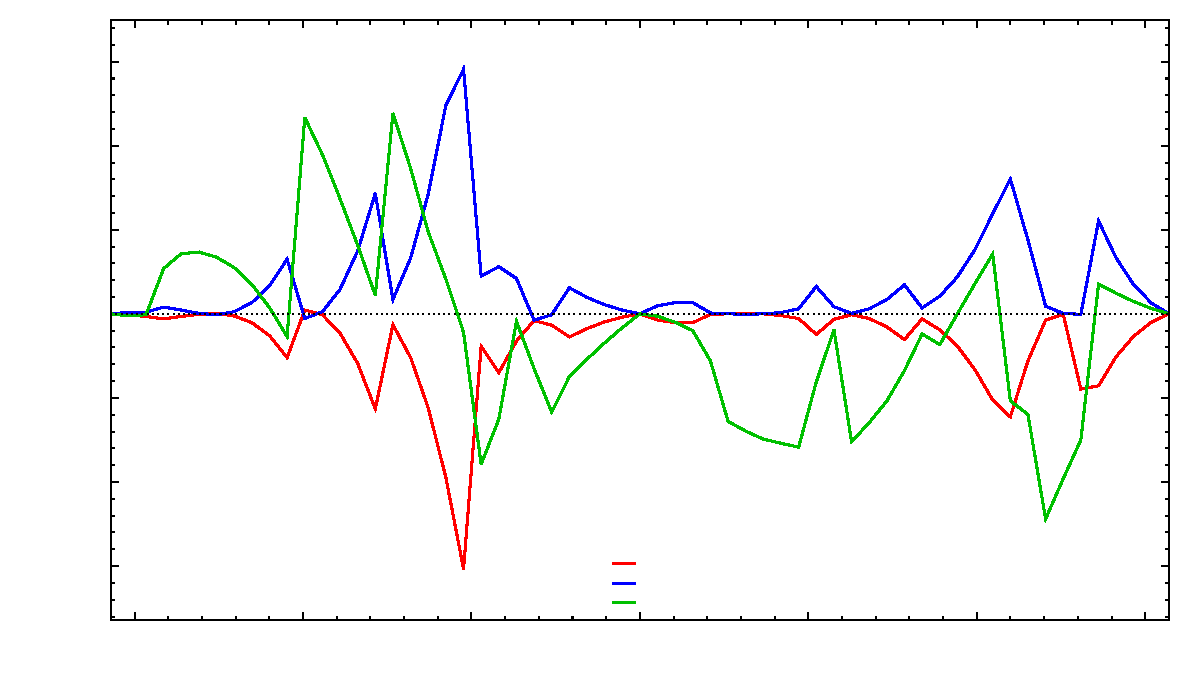
\includegraphics{pics/0_11a_11b_8_detail}}%
    \gplfronttext
  \end{picture}%
\endgroup
}
	\caption{Expected signifcance to exclude $\sin\delta_\text{CP} = 0$ for correlated (left) and anticorrelated (right) systematics.
		The anticorrelation between the $\nu_e$ and $\cj{\nu}_e$ CC cross-section systematic errors %
       		masks the resolution power to distinguihsing neutrino from anti-neutrino events. }
	\label{fig:0_11a_11b_8_sensitivity}
\end{figure}


\section{Dependencies on exclusion of CP}

Unknown mass hierachy, statistics ecc, octant determination.
